\documentclass[12pt,a4paper,final,twoside,titlepage]{book}
\usepackage[utf8]{inputenc}
\usepackage{amsmath}
\usepackage{algorithm2e}
\usepackage{amsfonts}
\usepackage{amssymb}
\usepackage{graphicx}
\usepackage{natbib}
\usepackage{listings}
\usepackage{color}
\usepackage{textcomp}
\usepackage{multirow}
\definecolor{listinggray}{gray}{0.9}
\definecolor{lbcolor}{rgb}{0.9,0.9,0.9}
\lstset{
	backgroundcolor=\color{white},
	tabsize=4,
	rulecolor=,
	language=csh,
        basicstyle=\scriptsize,
        upquote=true,
        aboveskip={1.5\baselineskip},
        columns=fixed,
        showstringspaces=false,
        extendedchars=true,
        breaklines=true,
        prebreak = \raisebox{0ex}[0ex][0ex]{\ensuremath{\hookleftarrow}},
        frame=single,
        showtabs=false,
        showspaces=false,
        showstringspaces=false,
        identifierstyle=\ttfamily,
        keywordstyle=\color[rgb]{0,0,1},
        commentstyle=\color[rgb]{0.133,0.545,0.133},
        stringstyle=\color[rgb]{0.627,0.126,0.941},
}
\author{Dr.Haitham A. El-Ghareeb}
\title{DATA STRUCTURES AND ALGORITHMS USING C\# AND PYTHON}
\begin{document}
\begin{titlepage}
\textbf{Dear Students...}\\
\textbf{\begin{center}
Welcome to the Course: Data Structures and Algorithms.
\end{center}}
It is always a pleasure, honor, and big responsibility to teach this course. Data Structures and Algorithms is one of the fundamental courses that shall help you traverse the world of Information and Computing in all fields: Computer Science, Information Systems, and Information Technology. Data Structures and Algorithms build over the:
\begin{itemize}
\item Introduction to Programming
\item Object Oriented Programming
\end{itemize}
To understand Data Structures and Algorithms well, you should have been introduced to: 
\begin{itemize}
\item Real world problems where we need Computer Science. Problems like Searching and Sorting to find the solution.
\item Systems where we need to store and retreive data from Information Systems. Problems like maintaining huge amount of data in memory needs to be very well considered.
\item Filling the gap between hardware and software efficiently through Information Technology needs fine utilization of hardware resources.
\end{itemize}
You might be familiar with the previous problems, and you might not! It is not a problem. To overcome this shortage, you will need to make more effort to catch up. Hopefully you are looking to catch up!
Object Oriented Programming is crucial for any programmer. However, it is not an emergency in this course. Though Object Oriented concepts, principles, and practicies are a need for programmers, you can survive this course without them. With one condition: Do more effort to follow the Object Oriented Concepts we are going to discuss through the book, and I assure you they are going to be the minimum as possible.\\
Data Structures and Algorithms Course has been for a long time, one of the courses I hope I will teach one day. It is the course that makes the difference between naive and professional programmer. In this course, we will learn many things, hopefully useful things.\\
Hope you will enjoy learning this course, the way I am enjoying teaching it.\\
\begin{flushright}
\textbf{Dr.Haitham A. El-Ghareeb\\
\textit{September 2012}}
\end{flushright}
\end{titlepage}
\tableofcontents
\listoffigures
\listoftables
\listofalgorithms
\part{REAL WORLD PROGRAMMING!}
\chapter{PROGRAMMING LANGUAGES ARE NOT THE SAME}
Programming languages are used for controlling the behavior of a machine (often a computer). Like natural languages, programming languages conform to rules for syntax and semantics. There are thousands of programming languages and new ones are created every year. Few languages ever become sufficiently popular that they are used by more than a few people, but professional programmers may use dozens of languages in a career. So, not to get lost between all those programming languages, there are main things we need to discuss in Programming Languages, and comparison between them.
\section{Basis for Comparing Programming Languages}
\subsection{Object Orientation}
Many languages claim to be Object-Oriented. While the exact definition of the term is highly variable, there are several qualities that most will agree an Object-Oriented language should have:
\begin{itemize}
\item Encapsulation/Information Hiding
\item Inheritance
\item Polymorphism/Dynamic Binding
\item All pre-defined types are Objects
\item All operations performed by sending messages to Objects
\item All user-defined types are Objects
\end{itemize}
A language is considered to be a "pure" Object-Oriented languages if it satisfies all of these qualities. A "hybrid" language may support some of these qualities, but not all. In particular, many languages support the first three qualities, but not the final three.

\subsection{Static vs. Dynamic Typing}
The debate between static and dynamic typing has raged in Object-Oriented circles for many years with no clear conclusion. Proponents of dynamic typing contend that it is more flexible and allows for increased productivity. Those who prefer static typing argue that it enforces safer, more reliable code, and increases efficiency of the resulting product.

Statically-typed language requires a very well-defined type system in order to remain as flexible as its dynamically-typed counterparts. Without the presence of genericity (templates) and multiple type inheritance, a static type system may severely inhibit the flexibility of a language. In addition, the presence of "casts" in a language can undermine the ability of the compiler to enforce type constraints.

A dynamic type system doesn't require variables to be declared as a specific type. Any variable can contain any value or object. In many cases this can make the software more flexible and amenable to change. However, care must be taken that variables hold the expected kind of object. Typically, if a variable contains an object of a different type than a user of the object expects, some sort of "message not understood" error is raised at run-time. Users of dynamically-typed languages claim that this type of error is infrequent in practice.

Statically-typed languages require that all variables are declared with a specific type. The compiler will then ensure that at any given time the variable contains only an object compatible with that type. (We say "compatible with that type" rather than "exactly that type" since the inheritance relationship enables subtyping, in which a class that inherits from another class is said to have an IS-A relationship with the class from which it inherits, meaning that instances of the inheriting class can be considered to be of a compatible type with instances of the inherited class.) By enforcing the type constraint on objects contained or referred to by the variable, the compiler can ensure a "message not understood" error can never occur at run-time. On the other hand, a static type system can hinder evolution of software in some circumstances. For example, if a method takes an object as a parameter, changing the type of the object requires changing the signature of the method so that it is compatible with the new type of the object being passed. If this same object is passed to many such methods, all of them must be updated accordingly, which could potentially be an arduous task. One must remember, though, that this ripple effect could occur even a dynamically-typed language. If the type of the object is not what it was originally expected to be, it may not understand the messages being sent to it. Perhaps even worse is that it could understand the message but interpret it in a way not compatible with the semantics of the calling method. A statically-typed language can flag these errors at compilation-time, pointing out the precise locations of potential errors. A user of a dynamically-typed language must rely on extensive testing to ensure that all improper uses of the object are tracked down.

\subsection{Generic Classes}
Generic classes, and more generally parametric type facilities, refer to the ability to parameterize a class with specific data types. A common example is a stack class that is parameterized by the type of elements it contains. This allows the stack to simultaneously be compile-time type safe and yet generic enough to handle any type of elements.

The primary benefit of parameterized types is that it allows statically typed languages to retain their compile-time type safety yet remain nearly as flexible as dynamically typed languages. Dynamically typed languages do not need parameterized types in order to support generic programming. Types are checked at run-time and thus dynamically typed languages support generic programming inherently.

\subsection{Inheritence}
Inheritance is the ability for a class or object to be defined as an extension or specialization of another class or object. Most object-oriented languages support class-based inheritance, while others such as SELF and JavaScript support object-based inheritance. A few languages, notably Python and Ruby, support both class- and object-based inheritance, in which a class can inherit from another class and individual objects can be extended at run time with the capabilities of other objects. 

Though there are identified and classified as many as 17 different forms of inheritance. Even so, most languages provide only a few syntactic constructs for inheritance which are general enough to allow inheritance to be used in many different ways. The most important distinction that can be made between various languages' support for inheritance is whether it supports single or multiple inheritance. Multiple inheritance is the ability for a class to inherit from more than one super (or base) class. For example, an application object called PersistentShape might inherit from both GraphicalObject and PersistentObject in order to be used as both a graphical object that can be displayed on the screen as well as a persistent object that can be stored in a database.

Multiple inheritance would appear to be an essential feature for a language to support for cases such as the above when two or more distinct hierarchies must be merged into one application domain. However, there are other issues to consider before making such an assertion.

First, we must consider that multiple inheritance introduces some complications into a programming language supporting it. Issues such as name clashes and ambiguities introduced in the object model must be resolved by the language in order for multiple inheritance and this leads to additional complexity in the language. 

Next, we must distinguish between implementation inheritance and interface/subtype inheritance. Subtype inheritance (also known loosely as interface inheritance) is the most common form of inheritance, in which a subclass is considered to be a subtype of its super class, commonly referred to as an IS-A relationship. What this means is that the language considers an object to conform to the type of its class or any of its super classes. For example, a Circle IS-A Shape, so anywhere a Shape is used in a program, a Circle may be used as well. This conformance notion is only applicable to statically typed languages since it is a feature used by the compiler to determine type correctness.

Implementation inheritance is the ability for a class to inherit part or all of its implementation from another class. For example, a Stack class that is implemented using an array might inherit from an Array class in order to define the Stack in terms of the Array. In this way, the Stack class could use any features from the Array to support its own implementation. With pure implementation inheritance, the fact that the Stack inherits its implementation from Array would not be visible to code using the Stack; the inheritance would be strictly an implementation matter. 

Returning to the issue of multiple inheritance, we can see that a language's support for multiple inheritance is not a boolean condition; a language can support one or more different forms of multiple inheritance in the same way it can support different forms of single inheritance (e.g. implementation and subtype inheritance). 

\subsection{Feature Renaming}
Feature renaming is the ability for a class or object to rename one of its features (a term used to collectively refer to attributes and methods) that it inherited from a super class. There are two important ways in which this can be put to use:
\begin{itemize}
\item Provide a feature with a more natural name for its new context
\item Resolve naming ambiguities when a name is inherited from multiple inheritance paths
\end{itemize}

\subsection{Method Overloading}
Method overloading (also referred to as parametric polymorphism) is the ability for a class, module, or other scope to have two or more methods with the same name. Calls to these methods are disambiguated by the number and/or type of arguments passed to the method at the call site. For example, a class may have multiple print methods, one for each type of thing to be printed. The alternative to overloading in this scenario is to have a different name for each print method, such as print\_string and print\_integer.

\subsection{Operator Overloading}
Operator overloading is the ability for a programmer to define an operator (such as +, or *) for user-defined types. This allows the operator to be used in infix, prefix, or postfix form, rather than the standard functional form. For example, a user-defined Matrix type might provide a * infix operator to perform matrix multiplication with the familiar notation: matrix1 * matrix2 .

Some (correctly) consider operator overloading to be mere syntactic "sugar" rather than an essential feature, while others (also correctly) point to the need for such syntactic sugar in numerical and other applications. Both points are valid, but it is clear that, when used appropriately, operator overloading can lead to much more readable programs. When abused, it can lead to cryptic, obfuscated code. Consider that in the presence of operator overloading, it may not be clear whether a given operator is built in to the language or defined by the user. For any language that supports operator overloading, two things are necessary to alleviate such obfuscation:

All operations must be messages to objects, and thus all operators are always method calls.
Operators must have an equivalent functional form, so that using the operator as a method call will behave precisely the same as using it in infix, prefix, or postfix form.

\subsection{Higher Order Functions \& Lexical Closures}
Higher order functions are, in the simplest sense, functions that can be treated as if they were data objects. In other words, they can be bound to variables (including the ability to be stored in collections), they can be passed to other functions as parameters, and they can be returned as the result of other functions. Due to this ability, higher order functions may be viewed as a form of deferred execution, wherein a function may be defined in one context, passed to another context, and then later invoked by the second context. This is different from standard functions in that higher order functions represent anonymous lambda functions, so that the invoking context need not know the name of the function being invoked.

Lexical closures (also known as static closures, or simply closures) take this one step further by bundling up the lexical (static) scope surrounding the function with the function itself, so that the function carries its surrounding environment around with it wherever it may be used. This means that the closure can access local variables or parameters, or attributes of the object in which it is defined, and will continue to have access to them even if it is passed to another module outside of its scope.

\subsection{Garbage Collection}
Garbage collection is a mechanism allowing a language implementation to free memory of unused objects on behalf of the programmer, thus relieving the burden on the programmer to do so. The alternative is for the programmer to explicitly free any memory that is no longer needed. There are several strategies for garbage collection that exist in various language implementations.
\subsubsection{Reference Counting}
Reference counting is the simplest scheme and involves the language keeping track of how many references there are to a particular object in memory, and deleting that object when that reference count becomes zero. This scheme, although it is simple and deterministic, is not without its drawbacks, the most important being its inability to handle cycles. Cycles occur when two objects reference each other, and thus there reference counts will never become zero even if neither object is referenced by any other part of the program.
\subsubsection{Mark and Sweep}
"Mark and sweep" garbage collection is another scheme that overcomes this limitation. A mark and sweep garbage collector works in a two phase process, known as the mark phase and the sweep phase. The mark phase works by first starting at the "root" objects (objects on the stack, global objects, etc.), marking them as live, and recursively marking any objects referenced from them. These marked objects are the set of live objects in program, and any objects that were not marked in this phase are unreferenced and therefore candidates for collection. In the sweep phase, any objects in memory that were not marked as live by the mark phase are deleted from memory. The primary drawback of mark and sweep collection is that it is non-deterministic, meaning that objects are deleted at an unspecified time during the execution of the program. This is the most common form of garbage collection.
\subsubsection{Generational}
Generational garbage collection works in a similar fashion to mark and sweep garbage collection, except it capitalizes on the statistical probability that objects that have been alive the longest tend to stay alive longer than objects that were newly created. Thus a generational garbage collector will divide objects into "generations" based upon how long they've been alive. This division can be used to reduce the time spent in the mark and sweep phases because the oldest generation of objects will not need to be collected as frequently. Generational garbage collectors are not as common as the other forms.

\subsection{Uniform Access}
The Uniform Access Principle, states that "All services offered by a module should be available through a uniform notation, which does not betray whether they are implemented through storage or through computation." It is described further with "Although it may at first appear just to address a notational issue, the Uniform Access principle is in fact a design rule which influences many aspects of object-oriented design and the supporting notation. It follows from the Continuity criterion; you may also view it as a special case of Information Hiding."

Say that \texttt{teach} is a feature of a class named \texttt{Professor}. For languages that do not support the Uniform Access Principle, the notation used to access \texttt{teach} differs depending on whether it is an attribute (storage) or a function (computation). For example, in Java we would use \texttt{Professor.teach} if it were an attribute, but we would use \texttt{Professor.teach()} if it were a function. Having this notational difference means that users of \texttt{Professor} are exposed to unnecessary implementation details and are tightly coupled to \texttt{Professor}. If \texttt{teach} is changed from attribute to method (or vice versa), then any users of \texttt{Professor} must also be changed.

The Uniform Access Principle seeks to eliminate this needless coupling. A language supporting the Uniform Access Principle does not exhibit any notational differences between accessing a feature regardless of whether it is an attribute or a function. Thus, in our earlier example, access to bar would always be in the form of foo.bar, regardless of how bar is implemented. This makes clients of Foo more resilient to change.

\subsection{Class Variables/Methods}
Class variables and methods are owned by a class, and not any particular instance of a class. This means that for however many instances of a class exist at any given point in time, only one copy of each class variable/method exists and is shared by every instance of the class.

\subsection{Reflection}
Reflection is the ability for a program to determine various pieces of information about an object at run-time. This includes the ability to determine the type of the object, its inheritance structure, and the methods it contains, including the number and types of parameters and return types. It might also include the ability for determining the names and types of attributes of the object. Most object-oriented languages support some form of reflection.

\subsection{Access Control}
Access control refers to the ability for a modules implementation to remain hidden behind its public interface. Access control is closely related to the encapsulation/information hiding principle of object-oriented languages. For example, a class \texttt{Professor} may have methods such as \texttt{name} and \texttt{email}, that return the professor's name and e-mail address respectively. How these methods work is an implementation detail that should not be available to users of the \texttt{Person} class. These methods may, for example, connect to a database to retrieve the values. The database connection code that is used to do this is not relevant to client code and should not be exposed. Language-enforced access control allows us to enforce this.
Most object-oriented languages provide at least two levels of access control: public and protected. Protected features are not available outside of the class in which they are contained, except for subclasses. Some languages, notably Java and C++, provide a third level of access control known as "private". Private features are not available outside of the class in which they are declared, even for subclasses. Note, however, that this means that objects of a particular class can access the private features of other objects of that same class. Java provides a fourth level of, known as "package private" access control which allows other classes in the same package to access such features.

\subsection{Design by Contract}
Design by Contract (DBC) is the ability to incorporate important aspects of a specification into the software that is implementing it. The most important features of DBC are:
\begin{itemize}
\item Pre-conditions, which are conditions that must be true before a method is invoked
\item Post-conditions, which are conditions guaranteed to be true after the invocation of a method
\item Invariants, which are conditions guaranteed to be true at any stable point during the lifetime of an object
\end{itemize}
There is much more to DBC than these simple facilities, including the manner in which pre-conditions, post-conditions, and invariants are inherited. However, at least these facilities must be present to support the central notions of DBC.

\subsection{Multithreading}
Multithreading is the ability for a single process to process two or more tasks concurrently. (We say concurrently rather than simultaneously because, in the absence of multiple processors, the tasks cannot run simultaneously but rather are interleaved in very small time slices and thus exhibit the appearance and semantics of concurrent execution.) The use of multithreading is becoming increasingly more common as operating system support for threads has become near ubiquitous.

\subsection{Regular Expressions}
Regular expressions are pattern matching constructs capable of recognizing the class of languages known as regular languages. They are frequently used for text processing systems as well as for general applications that must use pattern recognition for other purposes. Libraries with regular expression support exist for nearly every language, however it has become increasingly important for a language to support regular expressions natively. This allows tighter integration with the rest of the language and allows more convenient syntax for use of regular expressions. 

\subsection{Pointer Arithmetic}
Pointer arithmetic is the ability for a language to directly manipulate memory addresses and their contents. While, due to the inherent unsafety of direct memory manipulation, this ability is not often considered appropriate for high-level languages, it is essential for low-level systems applications. Thus, while object-oriented languages strive to remain at a fairly high level of abstraction, to be suitable for systems programming a language must provide such features or relegate such low-level tasks to a language with which it can interact. Most object-oriented languages have foregone support of pointer arithmetic in favor of providing integration with C. This allows low-level routines to be implemented in C while the majority of the application is written in the higher level language. C++ on the other hand provides direct support for pointer arithmetic, both for compatibility with C and to allow C++ to be used for systems programming without the need to drop down to a lower level language. This is the source both of C++'s great flexibility as well as much of its complexity.

\subsection{Language Integration}
For various reasons, including integration with existing systems, the need to interact with low level modules. It is important for a high level language (particularly interpreted languages) to be able to integrate seamlessly with other languages. Nearly every language to come along since C was first introduced provides such integration with C. This allows high level languages to remain free of the low level constructs that make C great for systems programming, but add much complexity.

\subsection{Built-In Security}
Built-in security refers to a language implementation's ability to determine whether or not a piece of code comes from a "trusted" source (such as the user's hard disk), limiting the permissions of the code if it does not. For example, Java applets are considered untrusted, and thus they are limited in the actions they can perform when executed from a user's browser. They may not, for example, read or write from or to the user's hard disk, and they may not open a network connection to anywhere but the originating host.

\section{Comparing based on Performance and Optimization}
Based on the previous basis for comparing programming languages, and because there are thousands of them, it is almost impossible to provide a comprehensive list of such features here. You, dear student, is encouraged to continue reserach in this point, and you are welcome to introduce such comparison between different programming lanuages of your choice in a report. Recent Google research \cite{Robert-Google} presents an important comparison between different programming languages. Through this important presented benchmark, differences between programming languages become clear. In this experience report, researcher encoded a well specified, compact benchmark in four programming languages, namely C++, Java, Go, and Scala. The implementations each use the languages' idiomatic container classes, looping constructs, and memory/object allocation schemes. It does not attempt to exploit specific language and run-time features to achieve maximum performance. This approach allows an almost fair comparison of language features, code complexity, compilers and compile time, binary sizes, run-times, and memory footprint. While the benchmark itself is simple and compact, it employs many language features, in particular, higher-level data structures (lists, maps, lists and arrays of sets and lists), a few algorithms (union/ find, dfs/deep recursion, and loop recognition based on Tarjan), iterations over collection types, some object oriented features, and interesting memory allocation patterns. Researcher did not explore any aspects of multi-threading, or higher level  type mechanisms, which vary greatly between the languages. The benchmark points to very large differences in all examined dimensions of the language implementations. After publication of the benchmark internally at Google, several engineers produced highly optimized versions of the benchmark. Researcher ound that in regards to performance, C++ wins out by a large margin. However, it also required the most extensive tuning efforts, many of which were done at a level of sophistication that would not be available to the average programmer. Scala concise notation and powerful language features allowed for the best optimization of code complexity. The Java version was probably the simplest to implement, but the hardest to analyze for performance. Specifically the effects around garbage collection were complicated and very hard to tune. Since Scala runs on the JVM, it has the same issues. Go offers interesting language features, which also allow for a concise and standardized notation. The compilers for this language are still immature, which reflects in both performance and binary sizes.

\section{Programming Languages of Choice}
Simply: C\# and Python.
\subsection{Why C\#?}
C\# (pronounced see sharp) is a multi-paradigm programming language encompassing strong typing, imperative, declarative, functional, generic, object-oriented (class-based), and component-oriented programming disciplines. It was developed by Microsoft within its .NET initiative and later approved as a standard by Ecma (ECMA-334) and ISO (ISO/IEC 23270:2006). C\# is one of the programming languages designed for the Common Language Infrastructure.
C\# is intended to be a simple, modern, general-purpose, object-oriented programming language. Its development team is led by Anders Hejlsberg. The most recent version is C\# 5.0, which was released on August 15, 2012.
\subsubsection{Design Goals}
The ECMA standard lists these design goals for C\#:
\begin{itemize}
\item C\# language is intended to be a simple, modern, general-purpose, object-oriented programming language.
\item The language, and implementations thereof, should provide support for software engineering principles such as strong type checking, array bounds checking, detection of attempts to use uninitialized variables, and automatic garbage collection. Software robustness, durability, and programmer productivity are important.
\item The language is intended for use in developing software components suitable for deployment in distributed environments.
\item Source code portability is very important, as is programmer portability, especially for those programmers already familiar with C and C++.
\item Support for internationalization is very important.
\item C\# is intended to be suitable for writing applications for both hosted and embedded systems, ranging from the very large that use sophisticated operating systems, down to the very small having dedicated functions.
\item Although C\# applications are intended to be economical with regard to memory and processing power requirements, the language was not intended to compete directly on performance and size with C or assembly language.
\end{itemize}

\subsection{Why Python?}


\section{Teach Yourself Programming in Ten Years}
Finally, and as a reminder, I encourage you to take a closer look on \cite{Peter-Norvig-10years}. To make it short, here is the receipe. So You Want to be a Programmer, here's Peter Norvig's recipe for programming success:
\begin{itemize}
\item Get interested in programming, and do some because it is fun. Make sure that it keeps being enough fun so that you will be willing to put in your ten years/10,000 hours.
\item Program. The best kind of learning is learning by doing. To put it more technically, "the maximal level of performance for individuals in a given domain is not attained automatically as a function of extended experience, but the level of performance can be increased even by highly experienced individuals as a result of deliberate efforts to improve." and "the most effective learning requires a well-defined task with an appropriate difficulty level for the particular individual, informative feedback, and opportunities for repetition and corrections of errors." 
\item Talk with other programmers; read other programs. This is more important than any book or training course.
If you want, put in four years at a college (or more at a graduate school). This will give you access to some jobs that require credentials, and it will give you a deeper understanding of the field, but if you don't enjoy school, you can (with some dedication) get similar experience on your own or on the job. In any case, book learning alone won't be enough. "Computer science education cannot make anybody an expert programmer any more than studying brushes and pigment can make somebody an expert painter" says Eric Raymond, author of The New Hacker's Dictionary. One of the best programmers I ever hired had only a High School degree; he's produced a lot of great software, has his own news group, and made enough in stock options to buy his own nightclub.
\item Work on projects with other programmers. Be the best programmer on some projects; be the worst on some others. When you're the best, you get to test your abilities to lead a project, and to inspire others with your vision. When you're the worst, you learn what the masters do, and you learn what they don't like to do (because they make you do it for them).
\item Work on projects after other programmers. Understand a program written by someone else. See what it takes to understand and fix it when the original programmers are not around. Think about how to design your programs to make it easier for those who will maintain them after you.
\item Learn at least a half dozen programming languages. Include one language that supports class abstractions (like Java or C++), one that supports functional abstraction (like Lisp or ML), one that supports syntactic abstraction (like Lisp), one that supports declarative specifications (like Prolog or C++ templates), one that supports coroutines (like Icon or Scheme), and one that supports parallelism (like Sisal).
\item Remember that there is a "computer" in "computer science". Know how long it takes your computer to execute an instruction, fetch a word from memory (with and without a cache miss), read consecutive words from disk, and seek to a new location on disk. (Answers here.)
\item Get involved in a language standardization effort. It could be the ANSI C++ committee, or it could be deciding if your local coding style will have 2 or 4 space indentation levels. Either way, you learn about what other people like in a language, how deeply they feel so, and perhaps even a little about why they feel so.
\item Have the good sense to get off the language standardization effort as quickly as possible.
\end{itemize}

\chapter{QUICK TOUR OF C\#}
\section{Introduction}
This chapter is not intended to be an extensive C\# course. We are presenting here the fundamentals needed to understand the rest of the code presented in the book. Obviously this book is primarily about Data Structures and Algorithms, but in several places we will explore some aspects of using IronPython with other .NET languages, the foremost being C\#. If you don’t know C\#, this chapter will give you a brief over- view of the core parts of the language. It should be enough to let you read the code examples in the book, although you’ll probably want more detail if you’re trying to write C\# code.
\section{Namespaces}
Namespaces are similar to other languages packages and modules. The classes in an assembly live in namespaces, which can be nested to provide a hierarchical structure. This structure is used to group together related classes to make them easier to find. Namespaces are specified in C\# like so:
\lstset{language=csh, tabsize=4}
\begin{lstlisting}
namespace DataStructures.Professor { 
	class Haitham { 
		... 
	}
}
\end{lstlisting}
Here we declare a namespace called \texttt{DataStructures.Professor}, which contains the \texttt{Haitham} class. Another major feature of namespaces is that they enable us to avoid name collisions: the fully qualified name of the class is \texttt{DataStructures.Professor.Haitham}, and we could happily use other \texttt{Haitham} classes in our project as long as they are in different namespaces.
\section{Classes}
Class declarations in C\# are structured like this:
\lstset{language=csh, tabsize=4}
 \begin{lstlisting}
public class Haitham: Professor, IBlogger, IMozillaReMo { 
	public string name; 
	public Haitham(string name) {
		this.name = name; // more fields and methods here
}
\end{lstlisting}
The access modifier public before the class keyword indicates that the class is accessible outside the current namespace. The names after the colon specify what this class inherits from. Haitham is a subclass of the Professor class, as well as the IBlogger and IMozillaReMo interfaces. C\# doesn’t allow multiple inheritance of classes, but implementing multiple interfaces is fine. If no parent class is specified in a class definition (or it inherits only from interfaces), the class inherits from \texttt{System.Object}. The body of the class can contain definitions of various kinds of members:
\begin{itemize}
\item Constructors 
\item Fields (like the name attribute in the previous snippet) 
\item Methods 
\item Properties 
\item Events 
\item Operators
\end{itemize}
Each of these members has access modifiers as well:
\begin{itemize}
\item private—Can be used only inside this class 
\item protected—Accessible from this class and any subclasses 
\item internal—Accessible from any class in the current assembly 
\item public—Available from any code
\end{itemize}
Classes can also contain other types (including classes, interfaces, structs, or dele- gates) as members.
As well as access modifiers, other modifiers can be applied to classes when they are defined:
\begin{itemize}
\item abstract—This declares that the class can be used only as a base class and can’t be instantiated. It might contain declarations of abstract methods (without any implementation) that subclasses must define when they are declared. (Abstract classes can still contain concrete implementations of some methods.)
\item static—This indicates that this class can’t be instantiated or used as a type (so it can’t be subclassed). Static classes are essentially containers for their members.
\item sealed—This prevents this class from being subclassed, for security or performance reasons. When the compiler sees a method call on a sealed class, it can generate a direct call to the method, rather than a virtual call.
\item partial—Partial classes are classes that are defined in more than one file. This can be useful if some code in a class is machine generated; the generated code can be kept in a separate file and regenerated without clobbering the custom code.
\end{itemize}
\section{Attributes}
Attributes are declarative information that can be attached to different elements of a program and examined at runtime using reflection. They can be applied to types, methods, and parameters, as well as other items. The .NET framework defines a number of attributes, such as SerializableAttribute, STAThreadAttribute, and FlagsAttribute, which control various aspects of how the code runs. You can also create new attributes (to be interpreted by your own code) by inheriting from System.Attribute.
The following code applies the SecretOverrideAttribute to the ProfessorHaitham.Teach method:
\lstset{language=csh, tabsize=4}
\begin{center}
 \begin{lstlisting}
class ProfessorHaitham { 
	//...
	[SecretOverride("...")] public void Teach(Subjects datastructures2012) {
	//...
	}
}
 \end{lstlisting}
\end{center}
\section{Interfaces}
An interface is a type that defines methods and properties with no behavior. Its purpose is to make a protocol explicit without imposing any other restrictions on the implementation. For example, the previous \texttt{ProfessorHaitham} class implements the IMozillaReMo interface:
\begin{lstlisting}
interface IMozillaReMo {
	IBrowser FavouriteBrowser {get; set;} 
	void Browse();
}
\end{lstlisting}
This means that \texttt{ProfessorHaitham} must provide a definition of the \texttt{FavouriteBrowser} property and the \texttt{Browse} method. Classes that implement multiple interfaces must provide definitions for all of the interfaces’ members. Interfaces can subclass other interfaces (and even inherit from multiple interfaces), which means that they include all of the members of their bases as well as the members they declare.
Ordinarily, a class that inherits from an interface can implement its members simply by defining them with the correct name, parameters, and return type. In some cases, you might not want the interface members to be part of your class’s interface (for example, if you have two different interfaces that clash). You can implement those members explicitly, so that they are available only when used through a reference to the interface:
\begin{lstlisting}
public class ExplicitlyDriveable: IMozillaReMo { 
	// member prefixed with interface name 
	public void IMozillaReMo.Browse() {
	// implementation here... 
	// other members
	}
}
\end{lstlisting}
Then code trying to use the \texttt{Browse} method on an ExplicitlyDriveable instance
must cast it to IMozillaReMo first.
\section{Enums}
Enumerations are collections of named constants, which look like this:
\begin{lstlisting}
enum CoursesITeach { 
	DataStructuresAndAlgorithms,
	SystemAnalysisAndDesign, 
	ResearchMethodologies, 
	DataBase
}
\end{lstlisting}
The enum values can be referred to in code using \texttt{CoursesITeach.DataStruct\\uresAndAlgorithms}. By default, enumerations inherit from int, but they can be declared (using the inheritance syntax) as any of the integral .NET types: sbyte, byte, short, ushort, int, uint, long, or ulong. Enums can be combined as flags with the bitwise-or operator (|) if you annotate them with the Flags attribute, in which case you should also specify the value of each member (by default, they’re assigned sequentially from 0). For example, if you wanted the \texttt{CoursesITeach} values to be combinable, you could define it as follows:
\begin{lstlisting}
[Flags] 
enum CoursesITeach {
	DataStructuresAndAlgorithms = 1, 
	SystemAnalysisAndDesign = 2, 
	ResearchMethodologies = 4, 
	DataBase = 8
}
\end{lstlisting}
\section{Struct}
Structs are data structures that are defined similarly to classes. The difference is that a struct is a value type rather than a reference type like a class. When a variable is of a class type, it contains a reference to an instance of the class (or null). A struct variable directly contains the members of the struct rather than being a reference to an object elsewhere in memory. This is generally useful for performance or memory optimization: a large array of structs can be much quicker to create than the same size array of objects. In some situations using structs can be slower, though, particularly when assigning or passing them as parameters (because all their member data needs to be copied). 
Struct definitions look like this:
\begin{lstlisting}
struct Faculty { 
	public float name; 
	public Faculty(String name) {
		//...
	}
}
\end{lstlisting}
Structs can’t inherit from any type (other than object, which they inherit from
implicitly), and no types can inherit from them.
\section{Methods}
Methods in C\# are members of classes and structs that are defined by giving the access level, the return type, the name of the method, and the parameters it accepts, as well as the block of code that is executed when it is called:
\begin{lstlisting}
class Haitham { 
	//...
	public void GoToLecture(string LectureName) { 
		Point location = this.targetDatabase.Find(targetName); 
		this.FlyToLocation(location);
	}
}
\end{lstlisting}
The void return type indicates that this method returns nothing.
\subsection{Virtual and override Methods}
The virtual modifier applied to a method indicates that it can be overridden in a subclass. The subclass’s version of the method must have the same visibility, name, parameter types, and return type as the base class method and be defined using the keyword override.
\begin{lstlisting}
class GiantRobot { 
	//...
	public virtual void TravelTo(Point destination) { 
		this.TurnTowards(destination); 
		while (this.Location != destination) {
			this.Trudge();
		}
	}
}

class FlyingRobot: GiantRobot { 
	//...
	public override void TravelTo(Point destination) { 
		if (this.WingState == WingState.Operational) {
			this.FlyTo(destination); 
			// whee! 
		} else {
			base.TravelTo(destination); // oh well...
		}	
	}
}
\end{lstlisting}
In a method, \texttt{this} refers to the current instance, although this doesn’t need to be a parameter of each method. To call a superclass method or property (for example, from the body of an override method), you refer to base. Semantics are simpler because any C\# class has only one superclass.
\subsection{Other method modifiers}
A number of other modifiers can be included after the access modifier when defining a method. The more commonly seen modifiers are these:
\begin{itemize}
\item static—This method must be called directly on the class rather than on an instance (and so can’t refer to this).
\item sealed—This override method can’t be overridden again in a subclass. This is often done for performance or security reasons.
\item abstract—This method must be implemented in subclasses. Abstract methods can’t contain any code.
\end{itemize}
\subsection{Parameter passing}
By default, method parameters are passed by object value (with the extra wrinkle that structs are copied).
In C\# you can change this behavior using the ref and out parameter modifiers. If a parameter has the ref modifier, it is passed by reference instead. Assignments to that parameter in the method will be reflected in the variable passed in by the caller. For example, an int variable passed as a ref parameter can be assigned in the method, and the variable’s value will be updated in the calling scope. Out parameters are similar, with the difference that they don’t need to be assigned a value before calling the method, and they must be assigned in the method. The difference between them is that out parameters are viewed as extra return values of the method, while ref parameters are values that are both input and potentially output of the method.
\section{Method overloading}
There can be multiple different methods in a class with the same name, as long as the combination of name and parameter types is unique within the class. Methods that have the same name but different parameters are said to be overloaded. When you call an overloaded method, the compiler uses the compile-time types of the parameters passed in to determine which version of the method is called. This is an important distinction between overload dispatch, where the selection of which overload to call is purely based on the declared types of the parameters, and method dispatch, where the method called is determined by the type of the instance at runtime, regardless of the declared type of the variable.
\section{Loops}
C\# has four looping constructs: while, do, for, and foreach.
\subsection{while loop}
The condition of the loop in C\# must evaluate to a bool.
\begin{lstlisting}
int a = 10; 
while (a > 0) {
	a--;
}
\end{lstlisting}
The loop control keywords break and continue work (for all C\# loops). The condition of the loop must be included in parentheses.
\subsection{do loop}
The do loop is like a while loop, where the condition is checked at the end of the loop body; that is, the loop body always executes at least once.
\begin{lstlisting}
int a = 0; 
do {
	a--; } while (a > 0);
\end{lstlisting}
After the execution of this loop, a will have the value -1.
\subsection{for loop}
The C\# for loop has three parts in addition to the loop body:
\begin{itemize}
\item An initialization clause, which sets up variables before the loop begins 
\item A condition that is tested before each execution of the loop body 
\item An iteration clause, which is executed after each execution of the loop body
\end{itemize}
Here’s an example:
\begin{lstlisting}
int total = 0; 
for (int i = 0; i < 10; i++) {
	total += i;
}
\end{lstlisting}
After execution, total will have the value 45 (the sum of 0 to 9), because it stops when i equals 1. Each of the three control clauses is optional, and each clause can consist of multiple statements separated by commas.
\subsection{foreach loop}
The foreach loop can iterate over any collection that implements the IEnumerable interface, including arrays.
\begin{lstlisting}
string[] names = new string[] {"Alice", "Bob", "Mallory"}; 
foreach (string person in names} {
	Console.WriteLine(person);
}
\end{lstlisting}
\section{if}
The condition must be in parentheses and yield a Boolean. If statements can be chained, so there’s no need for the elif.
\begin{lstlisting}
if (!robot.AtDestination()) { 
	robot.Walk();
} else if (robot.CanSee(target)) { 
		robot.Destroy(target);
	} else { 
		robot.ChillOut();
}
\end{lstlisting}
\section{switch}
Some situations that would require an if-elif-else construct or a dictionary lookup can be done more cleanly in C\# using a switch statement.
\begin{lstlisting}
MaterialSelection file; 
switch (target.Type) {
	case TargetType.DataStructuresAndAlgorithms: 
		book = "Data Structures and Algorithms using C\# and Python"; 
		break;
	case TargetType.DataBase: 
		book = "Database Management Systems, Thomas Conolley"; 
		break;
	case TargetType.ImageProcessing: 
	case TargetType.OpenCV:
		book = "Open CV Reference Book";
		break; 
	case default:
		book = null; 
		break;
\end{lstlisting}
The case labels must be constants, and each case has to end with a flow-control statement like break, throw, or return; execution isn’t allowed to fall through from one case to another. If you want fall-through behavior, you can use the goto case statement to explicitly jump to the case that should be executed. Two case labels together (like the ImageProcessing and OpenCV case shown previously) are treated as if they share the same body. If the switch expression doesn’t match any of the case labels and there’s a default case, it is executed.
\section{try/catch/finally and throw}
\begin{lstlisting}
try { 
	robot.ReturnToBase(TransportMode.FootThrusters);
} catch (FootThrusterFailure) { 
	robot.ReturnToBase(TransportMode.BoringWalking);
} catch (EmergencyOverrideException e) { 
	robot.SelectTarget(e.NewTarget);
} catch { robot.AssumeDefensivePosition(); 
	throw; // re-throw the original exception
} finally { 
	robot.NotifyBase();
}
\end{lstlisting}
\section{null}
null, a value that is the singleton instance of NoneType. null is a reference that doesn’t refer to any object. This has two consequences: first, null can be assigned to a variable of any reference type, and second, value types like int, DateTime, or custom structs can’t be null, because they don’t contain references.
The second fact can be inconvenient in some situations, so each value type in C\# has a nullable version, represented with the type name followed by a question mark. For example, a nullable integer variable would be declared with int?. Nullable types can then be used as normal (although there are performance differences under the hood) and be assigned null in the same way as reference types.
\section{Lab Excercises}
\textbf{Problem:}\\
If we list all the natural numbers below 10 that are multiples of 3 or 5, we get 3, 5, 6 and 9. The sum of these multiples is 23.
Find the sum of all the multiples of 3 or 5 below 1000.\\
\textbf{\textit{Hint:}} Answer: 233168\\
Thanks to http://projecteuler.net/problem=1
\textbf{Problem}
Write the Programs needed to solve the following problems:
\begin{itemize}
\item Program to compute $\sum_{i}^{n}=1^{i}$
\item Program to compute $\sum_{i}^{n}=1^{i}$ using Horner's rule.
\item Program to compute $\gamma$
\item Program to compute $\sum_{i}^{n}=x_{0}^{i}$
\item Program to compute $\sum_{i}^{n}=x_{0}^{i}$ using Horner's rule.
\item Program to compute $\sum_{i}^{n}=x_{0}^{i}$ using the closed-form expression.
\item Program to compute $\sum_{i=0}^{j}a_{i}$ for $0\leq j<n$
\item Program to compute $n!$
\end{itemize}

\part{BASIC DATA STRUCTURES}
\chapter{Collections and Generics}
\section{Collections}
A collection is a structured data type that stores data and provides operations for adding data to the collection. Operations include removing data from the collection, updating data in the collection, and operations for setting and returning the values of different attributes of the collection.
Collections can be broken down into two types: linear and nonlinear. A linear collection is a list of elements where one element follows the previous element. Elements in a linear collection are normally ordered by position (first, second, third, etc.). In the real world, a todo list is a good example of a linear collection; in the computer world (which is also real), an array is designed as a linear collection.
Nonlinear collections hold elements that do not have positional order within the collection. An organizational chart is an example of a nonlinear collection, as is a rack of billiard balls. In the computer world, trees, heaps, graphs, and sets are nonlinear collections.
Collections, be they linear or nonlinear, have a defined set of properties that describe them and operations that can be performed on them. An example of a collection property is the collections Count, which holds the number of items in the collection. Collection operations, called methods, include:
\begin{itemize}
\item Add (for adding a new element to a collection)
\item Insert (for adding a new element to a collection at a specified index)
\item Remove (for removing a specified element from a collection)
\item Clear (for removing all the elements from a collection)
\item Contains (for determining if a specified element is a member of a collection)
\item and IndexOf (for determining the index of a specified element in a collection).
\end{itemize} 
\section{Collection Types}
Within the two major categories of collections are several subcategories. Linear collections can be either direct access collections or sequential access collections, whereas nonlinear collections can be either hierarchical or grouped. This section describes each of these collection types.
\subsection{Linear Collections}
Linear Collections are broken into three major groups: Direct Access Collections, Sequential Access Collections, with a subtype called Generalized Access Collections.
\subsubsection{Direct Access Collections}
The most common example of a direct access collection is the array. We define an array as a collection of elements with the same data type that are directly accessed via an integer index, as illustrated in Figure \ref{Array} in page \pageref{Array}.
\begin{figure}
\begin{center}
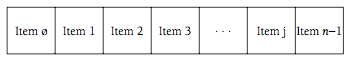
\includegraphics[scale=0.75]{Array}
\end{center}\caption{Array}
\label{Array}
\end{figure}
Arrays can be static so that the number of elements specified when the array is declared is fixed for the length of the program, or they can be dynamic, where the number of elements can be increased via the Array.Resize() method.
In C\#, arrays are not only a built-in data type, they are also a class. We can use an array to store a linear collection. Adding new elements to an array is easy since we simply place the new element in the first free position at the rear of the array. Inserting an element into an array is not as easy (or efficient), since we will have to move elements of the array down in order to make room for the inserted element. Deleting an element from the end of an array is also efficient, since we can simply remove the value from the last element. Deleting an element in any other position is less efficient because, just as with inserting, we will probably have to adjust many array elements up one position to keep the elements in the array contiguous. The .NET Framework provides a specialized array class, ArrayList, for making linear collection programming easier.
Another type of direct access collection is the string. A string is a collection of characters that can be accessed based on their index, in the same manner we access the elements of an array. Strings are also implemented as class objects in C\#. The class includes a large set of methods for performing standard operations on strings, such as concatenation, returning substrings, inserting characters, removing characters, and so forth.
C\# strings are immutable, meaning once a string is initialized it cannot be changed. When you modify a string, a copy of the string is created instead of changing the original string. This behavior can lead to performance degradation in some cases, so the .NET Framework provides a StringBuilder class that enables you to work with mutable strings. 
The final direct access collection type is the struct (also called structures and records in other languages). A struct is a composite data type that holds data that may consist of many different data types. For example, an employee record consists of employee’ name (a string), salary (an integer), identification number (a string, or an integer), as well as other attributes. Since storing each of these data values in separate variables could become confusing very easily, the language provides the struct for storing data of this type. A powerful addition to the C\# struct is the ability to define methods for performing operations stored on the data in a struct. This makes a struct somewhat like a class, though you can’t inherit or derive a new type from a structure. The following code demonstrates a simple use of a structure in C\#:
\begin{lstlisting}
using System; 
public struct Name { 
	private string fname, mname, lname;
	public Name(string first, string middle, string last) { 
		fname = first; 
		mname = middle; 
		lname = last;
	}
	public string firstName { 
		get {
			return fname;
		} 
		set {
			fname = firstName;
		}
	}	 
	public string middleName {
		get { 
			return mname;
		} 
		set {
			mname = middleName;
		}
	}
	public string lastName { 
		get {
			return lname;
		} 
		set {
			lname = lastName;
		}
	public override string ToString() { 
		return (String.Format("{0} {1} {2}", fname, mname, lname));
	}
	public string Initials() { 
		return (String.Format("{0}{1}{2}",fname.Substring(0,1), mname.Substring(0,1), lname.Substring(0,1)));
}

public class NameTest { static void Main() {
	Name myName = new Name("Haitham","A.","El-Ghareeb"); 
	string fullName, inits; 
	fullName = myName.ToString(); 
	inits = myName.Initials();
	Console.WriteLine("My name is {0}.", fullName); 
	Console.WriteLine("My initials are {0}.", inits);
	Console.ReadLine();
}
\end{lstlisting}
Although many of the elements in the .NET environment are implemented as classes (such as arrays and strings), several primary elements of the language are implemented as structures, such as the numeric data types. The Integer data type, for example, is implemented as the Int32 structure. One of the methods you can use with Int32 is the Parse method for converting the string representation of a number into an integer. Here’s an example:
\begin{lstlisting}
using System;
public class IntStruct { 
	static void Main() {
		int num; 
		string snum; 
		Console.Write("Enter a number: "); 
		snum = Console.ReadLine(); 
		num = Int32.Parse(snum); 
		Console.WriteLine(num);
		Console.ReadLine();
	}
}
\end{lstlisting}
\subsubsection{Sequential Access Collections}
A sequential access collection is a list that stores its elements in sequential order. We call this type of collection a linear list. Linear lists are not limited by size when they are created, meaning they are able to expand and contract dynamically. Items in a linear list are not accessed directly; they are referenced by their position, as shown in Figure \ref{LinearList} presented in page \pageref{LinearList}. The first element of a linear list is at the front of the list and the last element is at the rear of the list.
\begin{figure}
\begin{center}
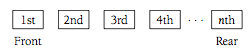
\includegraphics[scale=0.75]{LinearList}
\end{center}\caption{Linear List}
\label{LinearList}
\end{figure}
Because there is no direct access to the elements of a linear list, to access an element you have to traverse through the list until you arrive at the position of the element you are looking for. Linear list implementations usually allow two methods for traversing a list—in one direction from front to rear, and from both front to rear and rear to front.
A simple example of a linear list is a todo list. The list is created by writing down one item after another until the list is complete. The items are removed from the list while achieving as each item is completed.
Linear lists can be either ordered or unordered. An ordered list has values in order in respect to each other, as in:
\begin{center}
Beata Bernica David Frank Jennifer Mike Raymond Terrill
\end{center}
An unordered list consists of elements in any order. The order of a list makes a big difference when performing searches on the data on the list, as you’ll see later when we explore the binary search algorithm versus a simple linear search.
Some types of linear lists restrict access to their data elements. Examples of these types of lists are stacks and queues. A stack is a list where access is restricted to the beginning (or top) of the list. Items are placed on the list at the top and can only be removed from the top. For this reason, stacks are known as Last-in, First-out structures. When we add an item to a stack, we call the operation a push. When we remove an item from a stack, we call that operation a pop. These two stack operations are shown in Figure \ref{StackOperations} presented in page \pageref{StackOperations}.
\begin{figure}
\begin{center}
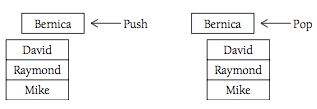
\includegraphics[scale=0.75]{StackOperations}
\end{center}
\caption{Stack Operations}
\label{StackOperations}
\end{figure}
The stack is a very common data structure, especially in computer systems programming. Stacks are used for arithmetic expression evaluation and for balancing symbols, among its many applications.
A queue is a list where items are added at the rear of the list and removed from the front of the list. This type of list is known as a First-in, First-out structure. Adding an item to a queue is called an EnQueue, and removing an item from a queue is called a Dequeue. Queue operations are shown in Figure \ref{QueueOperations} presented in page \pageref{QueueOperations}.
\begin{figure}
\begin{center}
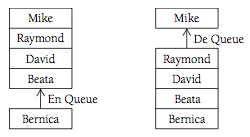
\includegraphics[scale=0.75]{QueueOperations}
\end{center}
\caption{Queue Operations}
\label{QueueOperations}
\end{figure}
Queues are used in both systems programming, for scheduling operating system tasks, and for simulation studies. Queues make excellent structures for simulating waiting lines in every conceivable retail situation. A special type of queue, called a priority queue, allows the item in a queue with the highest priority to be removed from the queue first. Priority queues can be used to study the operations of a hospital emergency room, where patients with heart trouble need to be attended to before a patient with a broken arm, for example.
\subsubsection{Generalized Indexed Collections}
The first of these, called a hash table, stores a set of data values associated with a key. In a hash table, a special function, called a hash function, takes one data value and transforms the value (called the key) into an integer index that is used to retrieve the data. The index is then used to access the data record associated with the key. For example, a doctor record may consist of a person’s name, his or her salary, the number of years the doctor has been with the university, and the department he or she works in. This structure is shown in Figure \ref{ARecordToBeHashed} presented in page \pageref{ARecordToBeHashed}. The key to this data record is the doctor's name. C\# has a class, called HashTable, for storing data in a hash table.
\begin{figure}
\begin{center}
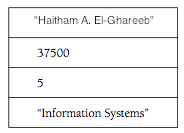
\includegraphics[scale=0.75]{ARecordToBeHashed}
\end{center}
\caption{A Record to be Hashed}
\label{ARecordToBeHashed}
\end{figure}
Another generalized indexed collection is the dictionary. A dictionary is made up of a series of key–value pairs, called associations. This structure is analogous to a word dictionary, where a word is the key and the word’s definition is the value associated with the key. The key is an index into the value associated with the key. Dictionaries are often called associative arrays because of this indexing scheme, though the index does not have to be an integer.
\subsection{Non Linear Collections}
Nonlinear collections are broken down into two major groups: hierarchical collections and group collections. 
\subsubsection{Hierarchichal Collections}
A hierarchical collection is a group of items divided into levels. An item at one level can have successor items located at the next lower level. One common hierarchical collection is the tree. A tree collection looks like an upside-down tree, with one data element as the root and the other data values hanging below the root as leaves. The elements of a tree are called nodes, and the elements that are below a particular node are called the node’s children. A sample tree is shown in Figure \ref{ATreeCollection} presented in page \pageref{ATreeCollection}. Trees have applications in several different areas. The file systems of most modern operating systems are designed as a tree collection, with one directory as the root and other subdirectories as children of the root.
A binary tree is a special type of tree collection where each node has no more than two children. A binary tree can become a binary search tree, making searches for large amounts of data much more efficient. This is accomplished by placing nodes in such a way that the path from the root to a node where the data is stored is along the shortest path possible.
Yet another tree type, the heap, is organized so that the smallest data value is always placed in the root node. The root node is removed during a deletion, and insertions into and deletions from a heap always cause the heap to reorganize so that the smallest value is placed in the root. Heaps are often used for sorts, called a heap sort. Data elements stored in a heap can be kept sorted by repeatedly deleting the root node and reorganizing the heap.
\begin{figure}
\begin{center}
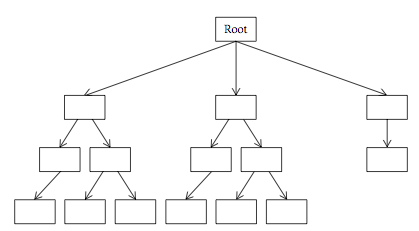
\includegraphics[scale=0.75]{ATreeCollection}
\end{center}
\caption{A Tree Collection}
\label{ATreeCollection}
\end{figure}
\subsubsection{Group Collections}
A nonlinear collection of items that are unordered is called a group. The three major categories of group collections are sets, graphs, and networks. A set is a collection of unordered data values where each value is unique. The list of students in a class is an example of a set, as is, of course, the integers. Operations that can be performed on sets include union and intersection. An example of set operations is shown in Figure \ref{SetCollectionOperations} presented in page \pageref{SetCollectionOperations}.
\begin{figure}
\begin{center}
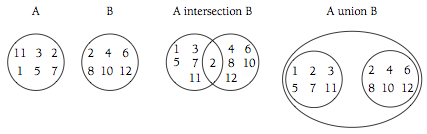
\includegraphics[scale=0.75]{SetCollectionOperations}
\end{center}
\caption{Set Collection Operations}
\label{SetCollectionOperations}
\end{figure}
A graph is a set of nodes and a set of edges that connect the nodes. Graphs are used to model situations where each of the nodes in a graph must be visited, sometimes in a particular order, and the goal is to find the most efficient way to “traverse” the graph. Graphs are used in logistics and job scheduling and are well studied by computer scientists and mathematicians. You may have heard of the “Traveling Salesman” problem. This is a particular type of graph problem that involves determining which cities on a salesman’s route should be traveled in order to most efficiently complete the route within the budget allowed for travel. A sample graph of this problem is shown in Figure \ref{TravelingSalesmanProblem} presented in page \pageref{TravelingSalesmanProblem}.
\begin{figure}
\begin{center}
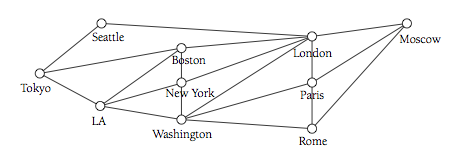
\includegraphics[scale=0.75]{TravelingSalesmanProblem}
\end{center}
\caption{The Traveling Salesman Problem}
\label{TravelingSalesmanProblem}
\end{figure}
This problem is part of a family of problems known as NP-complete problems. This means that for large problems of this type, an exact solution is not known. For example, to find the solution to the problem in Figure \ref{NetworkCollection} presented in page \pageref{NetworkCollection}, 10 factorial tours, which equals 3,628,800 tours. If we expand the problem to 100 cities, we have to examine 100 factorial tours, which we currently cannot do with current methods. An approximate solution must be found instead.
\begin{figure}
\begin{center}
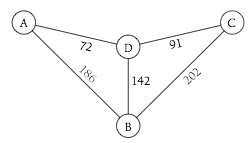
\includegraphics[scale=0.75]{NetworkCollection}
\end{center}
\caption{A Network Collection}
\label{NetworkCollection}
\end{figure}
A network is a special type of graph where each of the edges is assigned a weight. The weight is associated with a cost for using that edge to move from one node to another. Figure 1.9 depicts a network of cities where the weights are the miles between the cities (nodes).
We’ve now finished our tour of the different types of collections we are going to discuss in this book. Now we’re ready to actually look at how collections are implemented in C\#. We start by looking at how to build a Collection class using an abstract class from the .NET Framework, the CollectionBase class.

\subsection{Collection Class Implementation Using ArrayList}
The .NET Framework library does not include a generic Collection class for storing data, but there is an abstract class we can use to build our own Collection class—CollectionBase. The CollectionBase class provides the programmer with the ability to implement a custom Collection class. The class implicitly implements two interfaces necessary for building a Collection class, ICollection and IEnumerable, leaving the programmer with having to implement just those methods that are typically part of a Collection class.
In this section, we’ll demonstrate how to use C\# to implement our own Collection class. This will serve several purposes. First, if you’re not quite up to speed on object-oriented programming (OOP), this implementation will show you some simple OOP techniques in C\#. We can also use this section to discuss some performance issues that are going to come up as we discuss the different C\# data structures. It’s really a lot of fun to reimplement the existing data structures using just the native elements of the language. As Don Knuth (one of the pioneers of computer science) says, to paraphrase, you haven’t really learned something well until you’ve taught it to a computer. So, by teaching C\# how to implement the different data structures, we’ll learn much more about those structures than if we just choose to use the classes from the library in our day-to-day programming.
\subsection{Defining a Collection Class}
The easiest way to define a Collection class in C\# is to base the class on an abstract class already found in the System.Collections library—the Collection- Base class. This class provides a set of abstract methods you can implement to build your own collection. The CollectionBase class provides an underlying data structure, InnerList (an ArrayList), which you can use as a base for your class. In this section, we look at how to use CollectionBase to build a Collection class.
\subsection{Implementing the Collection Class}
The methods that will make up the Collection class all involve some type of interaction with the underlying data structure of the class—InnerList. The methods we will implement in this first section are the Add, Remove, Count, and Clear methods. These methods are absolutely essential to the class, though other methods definitely make the class more useful.
Let’s start with the Add method. This method has one parameter – an Object variable that holds the item to be added to the collection. Here is the code:
\begin{lstlisting}
public void Add(Object item) { 
	InnerList.Add(item);
}
\end{lstlisting}
ArrayLists store data as objects (the Object data type), which is why we have declared item as Object. You will learn much more about ArrayLists in the next chapter.
The Remove method works similarly:
\begin{lstlisting}
public void Remove(Object item) { 
	InnerList.Remove(item);
}
\end{lstlisting}
The next method is Count. Count is most often implemented as a property, but we prefer to make it a method. Also, Count is implemented in the underlying class, CollectionBase, so we have to use the new keyword to hide the definition of Count found in CollectionBase:
\begin{lstlisting}
public new int Count() { 
	return InnerList.Count;
}
\end{lstlisting}
The Clear method removes all the items from InnerList. We also have to use the new keyword in the definition of the method:
\begin{lstlisting}
public new void Clear() { 
	InnerList.Clear();
}
\end{lstlisting}
This is enough to get us started. Let’s look at a program that uses the Collection class, along with the complete class definition:
\begin{lstlisting}
using System; 
using System.Collections;
public class Collection<T> : CollectionBase { 
	public void Add(Object item) {
		InnerList.Add(item);
	} 
	public void Remove(Object item) {
		InnerList.Remove(item);
	} 
	public new void Clear() {
		InnerList.Clear();
	} 
	public new int Count() {
		return InnerList.Count;
	} 
}
class myCollection {
	static void Main() { 
		Collection<String> names = new Collection<String>(); 
		names.Add("Haitham"); 
		names.Add("Mohamed"); 
		names.Add("Ahmed"); 
		names.Add("Taha"); 
		foreach (Object name in names){
			Console.WriteLine(name); 
			Console.WriteLine("Number of names: " + names.Count()); 
		}		
		names.Remove("Taha");
		Console.WriteLine("Number of names: " + names. Count());
		names.Clear(); 
		Console.WriteLine("Number of names: " + names.Count());
		Console.ReadLine();
	}
}
\end{lstlisting}
\section{Generic Programming}
One of the problems with OOP is a feature called “code bloat.” One type of code bloat occurs when you have to override a method, or a set of methods, to take into account all of the possible data types of the method’s parameters. One solution to code bloat is the ability of one value to take on multiple data types, while only providing one definition of that value. This technique is called generic programming.
A generic program provides a data type “placeholder” that is filled in by a specific data type at compile-time. This placeholder is represented by a pair of angle brackets (< >), with an identifier placed between the brackets. Let’s look at an example.
A canonical first example for generic programming is the Swap function. Here is the definition of a generic Swap function in C\#:
\begin{lstlisting}
static void Swap<T>(ref T val1, ref T val2) { 
	T temp;
	temp = val1; 
	val1 = val2; 
	val2 = temp;
}
\end{lstlisting}
The placeholder for the data type is placed immediately after the function name. The identifier placed inside the angle brackets is now used whenever a generic data type is needed. Each of the parameters is assigned a generic data type, as is the temp variable used to make the swap. Here’s a program that tests this code:
\begin{lstlisting}
using System;
class genericsExample { 
	static void Main() {
		int num1 = 100; 
		int num2 = 200; 
		Console.WriteLine("num1: " + num1); 
		Console.WriteLine("num2: " + num2); 
		Swap<int>(ref num1, ref num2); 
		Console.WriteLine("num1: " + num1); 
		Console.WriteLine("num2: " + num2); 
		string str1 = "Haitham"; 
		string str2 = "El-Ghareeb"; 
		Console.WriteLine("String 1: " + str1); 
		Console.WriteLine("String 2: " + str2); 
		Swap<string>(ref str1, ref str2); 
		Console.WriteLine("String 1: " + str1); 
		Console.WriteLine("String 2: " + str2);
	}
	static void Swap<T>(ref T val1, ref T val2) { 
	T temp;
	temp = val1; 
	val1 = val2; 
	val2 = temp;
	}
}
\end{lstlisting}
Generics are not limited to function definitions; you can also create generic classes. A generic class definition will contain a generic type placeholder after the class name. Anytime the class name is referenced in the definition, the type placeholder must be provided. The following class definition demonstrates how to create a generic class:
\begin{lstlisting}
using System;
using System.Collections.Generic;
using System.Linq;
using System.Text;

namespace AnotherGenericExample
{
    public class Node<T>
    {
        T data;
        Node<T> link;
        public Node(T data, Node<T> link)
        {
            this.data = data;
            this.link = link;
        }
    }

    public class Program{
        static void Main(string[] args){
            Node<String> node1 = new Node<string>("El-Ghareeb", null);
            Node<String> node2 = new Node<string>("Haitham", node1);
            Console.WriteLine(node2);
            Console.ReadLine();
        }
    }
}
\end{lstlisting}
While this use of generic programming can be quite useful, C\# provides a library of generic data structures already ready to use. These data structures are found in the System.Collection.Generics namespace and when we discuss a data structure that is part of this namespace, we will examine its use. Generally, though, these classes have the same functionality as the nongeneric data structure classes, so we will usually limit the discussion of the generic class to how to instantiate an object of that class, since the other methods and their use are no different.
\section{Oversimplified Timing Tests}
This book takes both a practical and a theoritical approach to the analysis of the data structures and algorithms examined. We will use of Big O analysis later, however we are preferring  to run simple benchmark tests that will tell us how long in seconds (or whatever time unit) it takes for a code segment to run from the very beginning of the book. Our benchmarks will be timing tests that measure the amount of time it takes an algorithm to run to completion. Benchmarking is as much of an art as a science and you have to be careful how you time a code segment in order to get an accurate analysis. Benchmarking is the process of comparing one's business processes and performance metrics to industry bests or best practices from other industries. Dimensions typically measured are quality, time and cost. In the process of benchmarking, management identifies the best firms in their industry, or in another industry where similar processes exist, and compare the results and processes of those studied (the "targets") to one's own results and processes \cite{benchmarking-wikipedia}. In this way, they learn how well the targets perform and, more importantly, the business processes that explain why these firms are successful.
First, we need some code to time. For simplicity’s sake, we will time a sub-routine that writes the contents of an array to the console. Here’s the code:
\begin{lstlisting}
using System; 
using System.Diagnostics;

class testingTime
{
    static void Main()
    {
        Stopwatch myWatch = new Stopwatch();
        myWatch.Start();
        int[] nums = new int[1000000];
        BuildArray(nums);
        DisplayNums(nums);
        myWatch.Stop();
        Console.WriteLine("Elapsed MilliSeconds: " + myWatch.ElapsedMilliseconds.ToString());
        Console.WriteLine("Elapsed Seconds: " + myWatch.Elapsed.Seconds.ToString());
        Console.ReadLine();
    }
    static void BuildArray(int[] arr)
    {
        for (int i = 0; i <= 999999; i++)
            arr[i] = i;
    }
    static void DisplayNums(int[] arr)
    {
        for (int i = 0; i <= arr.GetUpperBound(0); i++)
            Console.Write(arr[i] + " ");
    }
}
\end{lstlisting}
Focusing on this code, we can notice that the core for calculating the time elapsed is:
\begin{lstlisting}
Using System;
Using System.Diagnostics;
Stopwatch watch = new Stopwatch();
watch.Start();
	//Execute the task to be timed
watch.Stop();
Console.WriteLine("Elapsed: {0}",watch.Elapsed);
Console.WriteLine("In milliseconds: {0}",watch.ElapsedMilliseconds);
Console.WriteLine("In timer ticks: {0}",watch.ElapsedTicks);
\end{lstlisting}
\section{Charting in .Net}
It would be nicer if we can create basic charts for timing results. We can use this charting in comparing the results. This section demonstrates how to add the Chart control to your Windows Forms application, and then add data, title, legends, and annotations to your chart. 
\subsection{Adding a Chart Control}
Follow the steps below to add a chart control to your Windows Forms application.
To add a chart control to your application:
\begin{enumerate}
\item In design view, open the Toolbox.
\item From the Data category, drag a Chart control to the design area.
If you cannot see the Chart control in the Toolbox, right click in the Toolbox, select Choose Items, and then select the following namespaces in the .NET Framekwork Components tab:
\begin{center}
System.Windows.Forms.DataVisualization.Charting 
\end{center}
\item Right-click the Chart control in the design area and select Properties.
\item In the Properties window, click the Categorized button.
\item In the Chart category of the Properties window, click the ChartAreas collection property, and then click the ellipsis button (…). This opens the ChartAreas Collection Editor.
The ChartAreas collection (a ChartAreaCollection object) contains all chart areas in the Chart control. Notice that the collection already contains a chart area named "ChartArea1".
\item Click Add, and then click OK. A new ChartArea object is added to the collection with the default name "ChartArea2".
Notice that the chart in the design area shrinks to half the original size. This is because the newly created chart area is placed at the bottom, but does not contain a data series yet.
\item In the Properties window, click the Series collection, and then click the ellipsis button. This opens the Series Collection Editor.
The Series collection (a SeriesCollection object) contains all data series in the Chart control. Notice that the collection already contains a series named "Series1".
\item In the Series Collection Editor, click Add, and then set the following properties with the newly created Series object as depicted in Table \ref{SeriesProperties} presented in page \pageref{SeriesProperties}
\begin{table}
\begin{center}
\caption{Chart Series Properties in .Net}
\begin{tabular}{|l|l|}
\hline Property & Value \\
\hline ChartArea & ChartArea2 \\
\hline ChartType & Bar \\
\hline Name & BarChart \\
\hline
\end{tabular}
\end{center}
\label{SeriesProperties}
\end{table}
\item Click OK, and then click OK again.
\end{enumerate}
Now there are chart areas, each chart area contains one data series. However, you will not see anything when you run your application because the series do not have any data yet.
\subsection{Adding Data to the Chart}
Follow the steps below to add data to the Chart control you just created.
To add data to the chart:
\begin{enumerate}
\item Open the Series Collection Editor again.
\item In the Members area, select Series1.
\item In the Data category of the Series1 properties area, click the Points collection property, and then click the ellipsis button. This opens the DataPoint Collection Editor.
\item The Points collection (a DataPointCollection object) contains all data points in the current series.
\item In the DataPoint Collection Editor, click Add, and then assign a value to the YValues property in the newly created DataPoint object.
\item Repeat this step until you have five data points in the collection.
\item Click OK, and then repeat the previous steps to add data points to the BarChart series.
\item In the Series Collection Editor, click OK.
\item Run your application.
Now you can see two chart areas in the Chart control displaying the data points you just created in the two series. Note the different chart types of the two series.
\end{enumerate}
\subsection{Adding Legends to the Chart}
Follow the steps below to add a legend for each series you just created.
To add a legend for each series
\begin{enumerate}
\item In the Chart category of the Properties window, click the Legends collection property, and then click the … button at the right. This opens the Legend Collection Editor.
The Legends collection (a LegendCollection object) contains all legends in the Chart control.
\item If there is not already a legend in the Legend Collection Editor, click Add.
\item Set the following properties with the Legend object as depicted in table \ref{LegendObjectProperties} presented in page \pageref{LegendObjectProperties}
\begin{table}
\begin{center}
\caption{Legend Object Properties in .Net}
\begin{tabular}{|l|l|}
\hline
DockedToChartArea & ChartArea1 \\ \hline
Docking & Right \\ \hline
IsDockedInsideChartArea & False\\ \hline
\end{tabular}
\end{center}
\label{LegendObjectProperties}
\end{table}
\item Click Add again, and then set the following properties with the newly created Legend object as depicted in table \ref{NewLegendObjectProperties} presented in page \pageref{NewLegendObjectProperties}
\begin{table}
\caption{New Legend Object Properties}
\label{NewLegendObjectProperties}
\begin{center}
\begin{tabular}{|l|l|}
\hline
DockedToChartArea & ChartArea2 \\ \hline
Docking & Right \\ \hline
\end{tabular}
\end{center}
\end{table}
\item Click OK.
Note that in the design area, the second legend is shown to be empty. By default, both series are assigned to the first legend. You can assign each series to a different legend.
\item Open the Series Collection Editor again.
\item In the Members area, select BarChart.
\item In the Legend category of the BarChart properties area, in the Legend property's dropdown list, select Legend2.
\item Click OK.
\item Run your application.
\end{enumerate}
\subsection{Adding a Title to the Chart}
Follow the steps below to add a title to your chart.
To add a title to the chart
\begin{enumerate}
\item In the Chart category of the Properties window, click the Titles collection property, and then click the ellipsis button. This opens the Title Collection Editor.
The Titles collection (a TitleCollection object) contains all titles in the Chart control.
\item In the Legend Collection Editor, click Add.
\item In the Appearance category of the Title1 properties area, type a chart title in the Text property.
\item Click OK.
\item Run your application.
\end{enumerate}
\subsection{Marking a Data Point with an Annotation}
Follow the steps below to use an annotation to mark a data point on the chart.
To mark a data point with an annotation
\begin{enumerate}
\item In the Chart category of the Properties window, click the Annotations collection property, and then click the ellipsis button. This opens the Annotation Collection Editor.
The Annotations collection (an AnnotationCollection object) contains all annotations in the Chart control.
\item In the Annotation Collection Editor, click the Add arrow and select ArrowAnnotation.
\item In the Anchor category of the ArrowAnnotation1 properties area, click the AnchorDataPoint arrow and select the first data point in Series1.
\item Set the following properties with the newly created Legend object as depicted in table \ref{LegendObjectProperties} presented in page \pageref{LegendObjectProperties}
\begin{table}
\begin{center}
\caption{Legend Object Properties}
\label{LegendObjectProperties}
\begin{tabular}{|l|l|}
\hline
Height & -5 \\ \hline
Width & 0 \\ \hline
AnchorOffSetY & -2.5 \\ \hline
\end{tabular}
\end{center}
\end{table}
\item In the Misc category, expand the SmartLabelStyle property and set its IsOverlappedHidden property to False.
\item Click OK.
\item Run your application.
\end{enumerate}
\subsection{Adding Series and Data at Run Time}
To add a series to the Chart control at run time, use the Add method in the Chart.Series collection property. To add a data point to a series at run time, use the Add, AddXY, and AddY methods in the Series.Points collection property.
The following code adds a column type series to the chart picture, adds a data point, and plots it in ChartArea1.
\begin{lstlisting}
Chart1.Series.Add("Series2");
Chart1.Series["Series2"].ChartType = SeriesChartType.Column;
Chart1.Series["Series2"].Points.AddY(20);
Chart1.Series["Series2"].ChartArea = "ChartArea1";
\end{lstlisting}
\section{Summary}
This chapter reviews three important techniques we will use often. Many, though not all of the programs we will write, as well as the libraries we will discuss, are written in an object-oriented manner. The Collection class we developed illustrates many of the basic OOP concepts seen throughout these chapters. Generic programming allows the programmer to simplify the definition of several data structures by limiting the number of methods that have to be written or overloaded. The Timing class provides a simple, yet effective way to measure the performance of the data structures and algorithms we will study.
\section{Practice}
From what you have learned, write the program needed to calculate the summation of numbers from:
\begin{itemize}
\item 1 - 10
\item 1 - 100
\item 1 - 1000
\item 1 - 10000
\item 1 - 100000
\item 1 - 1000000
\item 1 - 10000000
\end{itemize}
and draw the graph that illustrates the different consumed time solving this problem.
\section{Excercises}
\begin{enumerate}
\item Create a class called Test that has data members for a student’s name and a number indicating the test number. This class is used in the following scenario: When a student turns in a test, they place it face down on the desk. If a student wants to check an answer, the teacher has to turn the stack over so the first test is face up, work through the stack until the student’s test is found, and then remove the test from the stack. When the student finishes checking the test, it is reinserted at the end of the stack.
Write a Windows application to model this situation. Include text boxes for the user to enter a name and a test number. Put a list box on the form for displaying the final list of tests. Provide four buttons for the following actions: 
\begin{enumerate}
\item Turn in a test
\item Let student look at test
\item Return a test
\item and Exit.
\end{enumerate}
Perform the following actions to test your application: 
\begin{enumerate}
\item Enter a name and a test number. Insert the test into a collection named submittedTests
\item Enter a name, delete the associated test from submittedTests, and insert the test in a collection named outForChecking; \item Enter a name, delete the test from outForChecking, and insert it in submittedTests 
\item Press the Exit button. The Exit button doesn’t stop the application but instead deletes all tests from outForChecking and inserts them in submittedTests and displays a list of all the submitted tests.
\end{enumerate}
\item Add to the Collection class by implementing the following methods: 
\begin{enumerate}
\item Insert
\item Contains c. IndexOf
\item RemoveAt
\end{enumerate}
\end{enumerate}
\chapter{ARRAYS AND ARRAYLISTS}
\section{Introduction}
The array is the most common data structure, present in nearly all programming languages. Using an array in C\# involves creating an array object of System.Array type, the abstract base type for all arrays. The Array class provides a set of methods for performing tasks such as sorting and searching that programmers had to build by hand in the past.
An interesting alternative to using arrays in C\# is the ArrayList class. An arraylist is an array that grows dynamically as more space is needed. For situations where you can’t accurately determine the ultimate size of an array, or where the size of the array will change quite a bit over the lifetime of a program, an arraylist may be a better choice than an array.
In this chapter, we’ll quickly touch on the basics of using arrays in C\#, then move on to more advanced topics, including copying, cloning, testing for equality and using the static methods of the Array and ArrayList classes.

\section{Array Basics}
Arrays are indexed collections of data. The data can be of either a built-in type or a user-defined type. In fact, it is probably the simplest just to say that array data are objects. Arrays in C\# are actually objects themselves because they derive from the System.Array class. Since an array is a declared instance of the System.Array class, you have the use of all the methods and properties of this class when using arrays.
\subsection{Declaring and Initializing Arrays}
Arrays are declared using the following syntax:
\begin{lstlisting}
type[ ] array-name;
\end{lstlisting}
where type is the data type of the array elements. Here is an example:
\begin{lstlisting}
string[ ] names;
\end{lstlisting}
A second line is necessary to instantiate the array (since it is an object of System.Array type) and to determine the size of the array. The following line instantiates the names array just declared:
\begin{lstlisting}
names = new string[10];
\end{lstlisting}
and reserves memory for ten strings. You can combine these two statements into one line when necessary to do so:
\begin{lstlisting}
string[ ] names = new string[10];
\end{lstlisting}
There are times when you will want to declare, instantiate, and assign data to an array in one statement. You can do this in C\# using an initialization list:
\begin{lstlisting}
int[ ] numbers = new int[ ] {1,2,3,4,5};
\end{lstlisting}
The list of numbers, called the initialization list, is delimited with curly braces, and each element is delimited with a comma. When you declare an array using this technique, you don’t have to specify the number of elements. The compiler infers this data from the number of items in the initialization list.
\subsection{Setting and Accessing Array Elements}
Elements are stored in an array either by direct access or by calling the Array class method SetValue. Direct access involves referencing an array position by index on the left-hand side of an assignment statement:
\begin{lstlisting}
Names[2] = "Haitham"; 
professors[19] = 23123;
\end{lstlisting}
The SetValue method provides a more object-oriented way to set the value of an array element. The method takes two arguments, an index number and the value of the element.
\begin{lstlisting}
names.SetValue[2, "Haitham"]; 
professors.SetValue[19, 23123];
\end{lstlisting}
Array elements are accessed either by direct access or by calling the GetValue method. The GetValue method takes a single argument—an index.
\begin{lstlisting}
myName = names[2]; 
monthSalary = professors.GetValue[19];
\end{lstlisting}
It is common to loop through an array in order to access every array element using a For loop. A frequent mistake programmers make when coding the loop is to either hard-code the upper value of the loop (which is a mistake because the upper bound may change if the array is dynamic) or call a function that accesses the upper bound of the loop for each iteration of the loop:
\begin{lstlisting}
for (int i = 0; i <= professors.GetUpperBound(0); i++) {
	totalSalary = totalSalary + professors[i];
}
\end{lstlisting}
\subsection{Methods and Properties for Retrieving Array Metadata}
The Array class provides several properties for retrieving metadata about an array:
\begin{itemize}
\item Length: Returns the total number of elements in all dimensions of an array. 
\item GetLength: Returns the number of elements in specified dimension of an array.
\item Rank: Returns the number of dimensions of an array.
\item GetType: Returns the Type of the current array instance.
\end{itemize}
The Length method is useful for counting the number of elements in a multidimensional array, as well as returning the exact number of elements in the array. Otherwise, you can use the GetUpperBound method and add one to the value.
Since Length returns the total number of elements in an array, the GetLength method counts the elements in one dimension of an array. This method, along with the Rank property, can be used to resize an array at run-time without running the risk of losing data. This technique is discussed later in the chapter.
The GetType method is used for determining the data type of an array in a situation where you may not be sure of the array’s type, such as when the array is passed as an argument to a method. In the following code fragment, we create a variable of type Type, which allows us to use call a class method, IsArray, to determine if an object is an array. If the object is an array, then the code returns the data type of the array.
\begin{lstlisting}
int[ ] numbers;
numbers = new int[] {0,1,2,3,4}; 
Type arrayType = numbers.GetType(); 
if (arrayType.IsArray) {
	Console.WriteLine("The array type is: {0}", arrayType); 
} else {
    Console.WriteLine("Not an array");
}
  	Console.Read();
}
\end{lstlisting}
The GetType method returns not only the type of the array, but also lets us know that the object is indeed an array. Here is the output from the code:
\texttt{The array type is: System.Int32[]}
The brackets indicate the object is an array. Also notice that we use a format when displaying the data type. We have to do this because we can’t convert the Type data to string in order to concatenate it with the rest of the displayed string.
\section{Multidimensional Arrays}
So far we have limited our discussion to arrays that have just a single dimension. In C\#, an array can have up to 32 dimensions, though arrays with more than three dimensions are very rare (and very confusing). Multidimensional arrays are declared by providing the upper bound of each of the dimensions of the array. The two-dimensional declaration:
\texttt{int[,] grades = new int[4,5];}
declares an array that consists of 4 rows and 5 columns. Two-dimensional arrays are often used to model matrices.
You can also declare a multidimensional array without specifing the dimension bounds. To do this, you use commas to specify the number of dimensions. For example,\\
\texttt{double[,] Sales;}\\
declares a two-dimensional array, whereas\\
\texttt{double[,,] sales;}\\
declares a three-dimensional array. When you declare arrays without providing the upper bounds of the dimensions, you have to later redimension the array with those bounds:\\
\texttt{sales = new double[4,5];}\\
Multidimensional arrays can be initialized with an initialization list. Look at the following statement:\\
\begin{lstlisting}
Int[,] grades = new int[,] {{1, 82, 74, 89, 100}, 
										{2, 93, 96, 85, 86}, 
										{3, 83, 72, 95, 89}, 
										{4, 91, 98, 79, 88}}
\end{lstlisting}
First, notice that the upper bounds of the array are not specified. When you initialize an array with an initialization list, you can’t specify the bounds of the array. The compiler computes the upper bounds of each dimension from the data in the initialization list. The initialization list itself is demarked with curly braces, as is each row of the array. Each element in the row is delimited with a comma.
Accessing the elements of a multidimensional array is similar to accessing the elements of a one-dimensional array. You can use the traditional array access technique,\\
\texttt{grade = Grades[2,2];\\Grades(2,2) = 99}
or you can use the methods of the Array class:\\
\texttt{grade = Grades.GetValue[0,2]}
You can’t use the SetValue method with a multidimensional array because the method only accepts two arguments: a value and a single index.
It is a common operation to perform calculations on all the elements of a multidimensional array, though often based on either the values stored in the rows of the array or the values stored in the columns of the array. Using the Grades array, if each row of the array is a student record, we can calculate the grade average for each student as follows:
\begin{lstlisting}
int[,] grades = new int[,] {{1, 82, 74, 89, 100}, 
							{2, 93, 96, 85, 86}, 
							{3, 83, 72, 95, 89},
							{4, 91, 98, 79, 88}}; 
int last_grade = grades.GetUpperBound(1);
double average = 0.0;
int total;
int last_student = grades.GetUpperBound(0); 
for(int row = 0; row <= last_student; row++) {
    total = 0;
    for (int col = 0; col <= last_grade; col++)
      total += grades[row, col];
      average = total / last_grade;
      Console.WriteLine("Average: " + average);
	}
 }
\end{lstlisting}

\section{Parameter Arrays}
Most method definitions require that a set number of parameters be provided to the method, but there are times when you want to write a method definition that allows an optional number of parameters. You can do this using a construct called a parameter array. A parameter array is specified in the parameter list of a method definition by using the keyword ParamArray. The following method definition allows any amount of numbers to be supplied as parameters, with the total of the numbers returned from the method:
\begin{lstlisting}
static int sumNums(params int[] nums) {
int sum = 0;
for(int i = 0; i <= nums.GetUpperBound(0); i++)
      sum += nums[i];
    return sum;
}
\end{lstlisting}
This method will work with the either of the following calls:\\
\texttt{total = sumNums(1, 2, 3); \\total = sumNums(1, 2, 3, 4, 5, 6, 7, 8, 9, 10);}
When you define a method using a parameter array, the parameter array arguments have to be supplied last in the parameter list in order for the compiler to be able to process the list of parameters correctly. Otherwise, the compiler wouldn’t know the ending point of the parameter array elements and the beginning of other parameters of the method.

\section{Jagged Arrays}
When you create a multidimensional array, you always create a structure that has the same number of elements in each of the rows. For example, look at the following array declaration:\\
\texttt{int sales[,] = new int[12,30]; ' Sales for each day of each month}
This array assumes each row (month) has the same number of elements (days), when we know that some months have 30 days, some have 31, and one month has 29. With the array we’ve just declared, there will be several empty elements in the array. This isn’t much of a problem for this array, but with a much larger array we end up with a lot of wasted space.
The solution to this problem is to use a jagged array instead of a two-dimensional array. A jagged array is an array of arrays where each row of an array is made up of an array. Each dimension of a jagged array is a one-dimensional array. We call it a “jagged” array because the number of elements in each row may be different. A picture of a jagged array would not be square or rectangular, but would have uneven or jagged edges.
A jagged array is declared by putting two sets of parentheses after the array variable name. The first set of parentheses indicates the number of rows in the array. The second set of parentheses is left blank. This marks the place for the one-dimensional array that is stored in each row. Normally, the number of rows is set in an initialization list in the declaration statement, like this:\\
\texttt{int[][] jagged = new int[12][];}\\
This statement looks strange, but makes sense when you break it down. jagged is an Integer array of 12 elements, where each of the elements is also an Integer array. The initialization list is actually just the initialization for the rows of the array, indicating that each row element is an array of 12 elements, with each element initialized to the default value.
Once the jagged array is declared, the elements of the individual row arrays can be assigned values. The following code fragment assigns values to jaggedArray:\\
\texttt{jagged[0][0] = 23; \\jagged[0][1] = 13; \\... \\jagged[7][5] = 45;}\\
The first set of parentheses indicates the row number and the second set indicates the element of the row array. The first statement accesses the first element of the first array, the second element access the second element of the first array, and the third statement accesses the sixth element of the eighth array.
For an example of using a jagged array, the following program creates an array named sales (tracking one week of sales for two months), assigns sales figures to its elements, and then loops through the array to calculate the average sales for one week of each of the two months stored in the array.
\begin{lstlisting}
using System; 
class class1 {
	static void Main[] {
		int[] Jan = new int[31];
		int[] Feb = new int[29];
		int[][] sales = new int{Jan, Feb}; 
		int month, day, total;
		double average = 0.0;
		sales[0][0] = 41;
		sales[0][1] = 30;
		sales[0][0] = 41;
		sales[0][1] = 30;
		sales[0][2] = 23;
		sales[0][3] = 34;
		sales[0][4] = 28;
		sales[0][5] = 35;
		sales[0][6] = 45;
		sales[1][0] = 35;
		sales[1][1] = 37;
		sales[1][2] = 32;
		sales[1][3] = 26;
		sales[1][4] = 45;
		sales[1][5] = 38;
		sales[1][6] = 42;
		for(month = 0; month <= 1; month++) {
      		total = 0;
      		for(day = 0; day <= 6; day++) {
        		total += sales[month][day];
        	}
        }
      	average = total / 7;
   		Console.WriteLine("Average sales for month: " + month + ": " + average);
	}
}
\end{lstlisting}
\section{The ArrayList Class}
Static arrays are not very useful when the size of an array is unknown in advance or is likely to change during the lifetime of a program. One solution to this problem is to use a type of array that automatically resizes itself when the array is out of storage space. This array is called an ArrayList and it is part of the System.Collections namespace in the .NET Framework library.
An ArrayList object has a Capacity property that stores its size. The initial value of the property is 16. When the number of elements in an ArrayList reaches this limit, the Capacity property adds another 16 elements to the storage space of the ArrayList. Using an ArrayList in a situation where the number of elements in an array can grow larger, or smaller, can be more efficient than using Array.Resize Preserver with a standard array. ArrayList stores objects using the Object type. If you need a strongly typed array, you should use a standard array or some other data structure.
\subsection{Example of Using ArrayList Class}
The following example shows how to create and initialize an ArrayList and how to print out its values.
\begin{lstlisting}
using System;
using System.Collections;
public class SamplesArrayList  {

   public static void Main()  {

      // Creates and initializes a new ArrayList.
      ArrayList myAL = new ArrayList();
      myAL.Add("Hello");
      myAL.Add("World");
      myAL.Add("!");

      // Displays the properties and values of the ArrayList.
      Console.WriteLine( "myAL" );
      Console.WriteLine( "\tCount:    {0}", myAL.Count );
      Console.WriteLine( "\tCapacity: {0}", myAL.Capacity );
      Console.Write( "\tValues:" );
      PrintValues( myAL );
   }

   public static void PrintValues( IEnumerable myList )  {
      System.Collections.IEnumerator myEnumerator = myList.GetEnumerator();
      while ( myEnumerator.MoveNext() )
         Console.Write( "\t{0}", myEnumerator.Current );
      Console.WriteLine();
   }
}
/* 
This code produces the following output.

myAL
    Count:    3
    Capacity: 16
    Values:    Hello    World    !
*/
\end{lstlisting}
\subsection{ArrayList Class Propoerties}
The ArrayList class includes several methods and properties for working with ArrayLists. Here is a list of some of the most commonly used methods and properties:
\begin{itemize}
\item Capacity: Gets or sets the number of elements that the ArrayList can contain.
\item Count: Gets the number of elements actually contained in the ArrayList.
\item IsFixedSize: Gets a value indicating whether the ArrayList has a fixed size.
\item IsReadOnly: Gets a value indicating whether the ArrayList is read-only.
\item IsSynchronized: Gets a value indicating whether access to the ArrayList is synchronized (thread-safe).
\item Item: Gets or sets the element at the specified index. In C\#, this property is the indexer for the ArrayList class.
\item SyncRoot: Gets an object that can be used to synchronize access to the ArrayList.
\end{itemize}
\subsection{ArralyList Class Methods}
\begin{itemize}
\item Adapter: Creates an ArrayList wrapper for a specific IList.
\item Add: Adds an object to the end of the ArrayList.
\item AddRange: Adds the elements of an ICollection to the end of the ArrayList.
\item BinarySearch: Overloaded. Uses a binary search algorithm to locate a specific element in the sorted ArrayList or a portion of it.
\item Clear: Removes all elements from the ArrayList.
\item Clone: Creates a shallow copy of the ArrayList.
\item Contains: Determines whether an element is in the ArrayList.
\item CopyTo: Overloaded. Copies the ArrayList or a portion of it to a one-dimensional array.
\item Equals (inherited from Object): Overloaded. Determines whether two Object instances are equal.
\item FixedSize: Overloaded. Returns a list wrapper with a fixed size, where elements are allowed to be modified, but not added or removed.
\item GetEnumerator: Overloaded. Returns an enumerator that can iterate through the ArrayList.
\item GetHashCode (inherited from Object): Serves as a hash function for a particular type, suitable for use in hashing algorithms and data structures like a hash table.
\item GetRange: Returns an ArrayList which represents a subset of the elements in the source ArrayList.
\item GetType (inherited from Object): Gets the Type of the current instance.
\item IndexOf: Overloaded. Returns the zero-based index of the first occurrence of a value in the ArrayList or in a portion of it.
\item Insert: Inserts an element into the ArrayList at the specified index.
\item InsertRange: Inserts the elements of a collection into the ArrayList at the specified index.
\item LastIndexOf: Overloaded. Returns the zero-based index of the last occurrence of a value in the ArrayList or in a portion of it.
\item ReadOnly: Overloaded. Returns a list wrapper that is read-only.
\item Remove: Removes the first occurrence of a specific object from the ArrayList.
\item RemoveAt: Removes the element at the specified index of the ArrayList.
\item RemoveRange: Removes a range of elements from the ArrayList.
\item Repeat: Returns an ArrayList whose elements are copies of the specified value.
\item Reverse: Overloaded. Reverses the order of the elements in the ArrayList or a portion of it.
\item SetRange: Copies the elements of a collection over a range of elements in the ArrayList.
\item Sort: Overloaded. Sorts the elements in the ArrayList or a portion of it.
\item Synchronized: Overloaded. Returns a list wrapper that is synchronized (thread-safe).
\item ToArray: Overloaded. Copies the elements of the ArrayList to a new array.
\item ToString (inherited from Object): Returns a String that represents the current Object.
\item TrimToSize: Sets the capacity to the actual number of elements in the ArrayList.
\item Finalize (inherited from Object): Overridden. Allows an Object to attempt to free resources and perform other cleanup operations before the Object is reclaimed by garbage collection. In C\# and C++, finalizers are expressed using destructor syntax.
\item MemberwiseClone (inherited from Object): Supported by the .NET Compact Framework. Creates a shallow copy of the current Object.
\end{itemize}

\section{Memory Management of Arrays}
To help understand how the .NET Framework stores the internals of an array, consider the following example:
\begin{lstlisting}
bool [] booleanArray;
FileInfo [] files;
booleanArray = new bool[10];
files = new FileInfo[10];
\end{lstlisting}
Here, the booleanArray is an array of the value type System.Boolean, while the files array is an array of a reference type, System.IO.FileInfo. Figure \ref{CLR-Value} presented in page \pageref{CLR-Value} shows a depiction of the CLR-managed heap after these four lines of code have executed.
\begin{figure}
\begin{center}
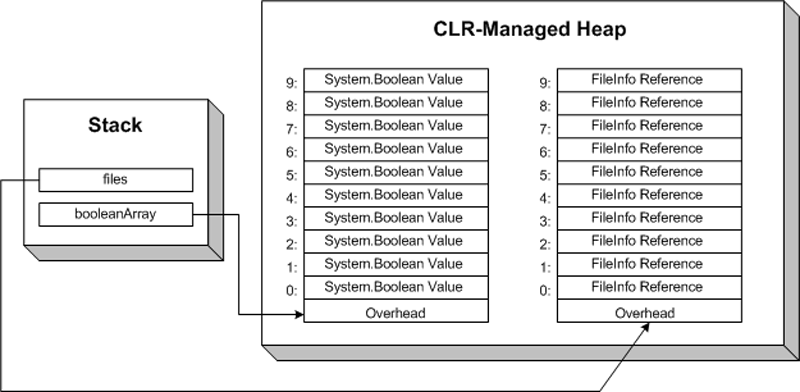
\includegraphics[scale=0.5]{CLR-Value}
\caption{The contents of an array are laid out contiguously in the managed heap.}
\label{CLR-Value}
\end{center}
\end{figure}
The thing to know is that the ten elements in the files array are references to FileInfo instances. Figure  \ref{CLR-Value2} presented in page \pageref{CLR-Value2} explains this point, showing the memory layout if we assign some of the values in the files array to FileInfo instances.
\begin{figure}
\begin{center}
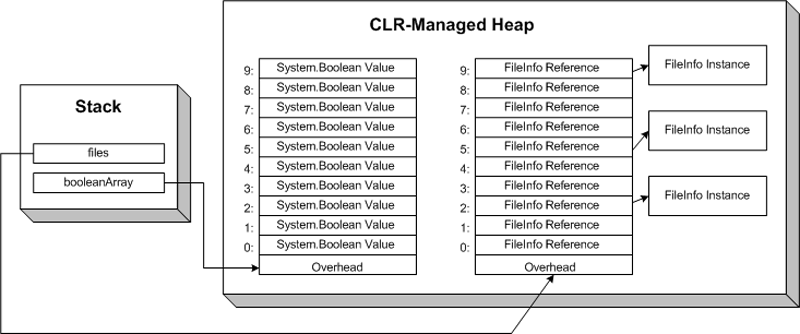
\includegraphics[scale=0.5]{CLR-Value2}
\caption{The contents of an array are laid out contiguously in the managed heap.}
\label{CLR-Value2}
\end{center}
\end{figure}
\section{Memory Management of ArrayList}
While the ArrayList provides added flexibility over the standard array, this flexibility comes at the cost of performance, especially when storing value types in an ArrayList. Recall that an array of a value type—such as a System.Int32, System.Double, System.Boolean, and so on—is stored contiguously in the managed heap in its unboxed form. The ArrayList's internal array, however, is an array of object references. Therefore, even if you have an ArrayList that stores nothing but value types, each ArrayList element is a reference to a boxed value type, as shown in Figure \ref{CLR-Value3} presented in page \pageref{CLR-Value3}
\begin{figure}
\begin{center}
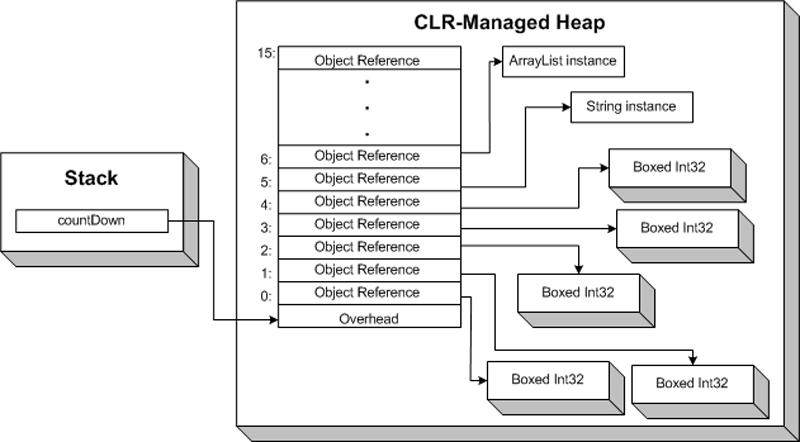
\includegraphics[scale=0.5]{CLR-Value3}
\caption{The ArrayList contains a contiguous block of object references.}
\label{CLR-Value3}
\end{center}
\end{figure}
The boxing and unboxing, along with the extra level of indirection that comes with using value types in an ArrayList, can hamper the performance of your application when using large ArrayLists with many reads and writes. As Figure 3 illustrates, the same memory layout occurs for reference types in both ArrayLists and arrays.


\section{Summary}
The array is the most commonly used data structure in computer program- ming. Most, if not all, computer languages provide some type of built-in array. For many applications, the array is the easiest data structure to implement and the most efficient. Arrays are useful in situations where you need direct access to “far away” elements of your data set.
The .NET Framework introduces a new type of array called an ArrayList. ArrayLists have many of the features of the array, but are somewhat more powerful because they can resize themselves when the current capacity of the structure is full. The ArrayList also has several useful methods for performing insertions, deletions, and searches. Since C\# does not allow a programmer to dynamically resize an array as you can in VB.NET, the ArrayList is a useful data structure for situations where you can’t know in advance the total number of items for storage.
\section{Excercises}
\begin{enumerate}
\item Design and implement a class that allows a teacher to track the grades in a single course. Include methods that calculate the average grade, the highest grade, and the lowest grade. Write a program to test your class implementation.
\item Modify Exercise 1 so that the class can keep track of multiple courses. Write a program to test your implementation.
\item Rewrite Exercise 1 using an ArrayList. Write a program to test your imple- mentation and compare its performance to that of the array implementation in Exercise 1 using the Timing class.
\item Design and implement a class that uses an array to mimic the behavior of the ArrayList class. Include as many methods from the ArrayList class as possible. Write a program to test your implementation.
\end{enumerate}
\chapter{Stacks and Queues}
\section{Introduction}
Data organize naturally as lists. We have already used the Array and ArrayList classes for handling data organized as a list. Although those data structures helped us group the data in a convenient form for processing, neither structure provides a real abstraction for actually designing and implementing problem solutions.
Two list-oriented data structures that provide easy-to-understand abstractions are stacks and queues. Data in a stack are added and removed from only one end of the list, whereas data in a queue are added at one end and removed from the other end of a list. Stacks are used extensively in programming language implementations, from everything from expression evaluation to handling function calls. Queues are used to prioritize operating system processes and to simulate events in the real world, such as teller lines at banks and the operation of elevators in buildings.
C\# provides two classes for using these data structures: the Stack class and the Queue class.
\section{Stacks}
The stack is one of the most frequently used data structures, as we just men- tioned. We define a stack as a list of items that are accessible only from the end of the list, which is called the top of the stack. The standard model for a stack is the stack of trays at a cafeteria. Trays are always removed from the top, and the when the dishwasher or busboy puts a tray back on the stack, it is placed on the top also. A stack is known as a Last-in, First-out (LIFO) data structure.
\subsection{Stack Operations}
The two primary operations of a stack are adding items to the stack and taking items off the stack. The Push operation adds an item to a stack. We take an item off the stack with a Pop operation. These operations are illustrated in Figure \ref{Stack} presented in \pageref{Stack}.
\begin{figure}
\begin{center}
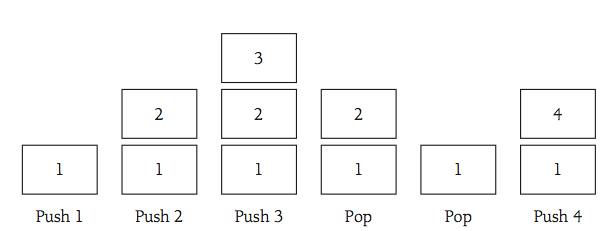
\includegraphics[scale=0.5]{Stack}
\caption{Stack Two Main Operations: Push, and Pop}
\label{Stack}
\end{center}
\end{figure}
The other primary operation to perform on a stack is viewing the top item. The Pop operation returns the top item, but the operation also removes it from the stack. We want to just view the top item without actually removing it. This operation is named Peek in C\#, though it goes by other names in other languages and implementations (such as Top).
Pushing, popping, and peeking are the primary operations we perform when using a stack; however, there are other operations we need to perform and properties we need to examine. It is useful to be able to remove all the items from a stack at one time. A stack is completed emptied by calling the Clear operation. It is also useful to know how many items are in a stack at any one time. We do this by calling the Count property. Many implementations have a StackEmpty method that returns a true or false value depending on the state of the stack, but we can use the Count property for the same purposes.
The Stack class of the .NET Framework implements all of these operations and properties and more, but before we examine how to use them, let’s look at how you would have to implement a stack if there wasn’t a Stack class.
\subsection{Stack Constructors}
\begin{itemize}
\item Stack(): Initializes a new instance of the Stack class that is empty and has the default initial capacity.
\item Stack(ICollection): Initializes a new instance of the Stack class that contains elements copied from the specified collection and has the same initial capacity as the number of elements copied.
\item Stack(Int32): Initializes a new instance of the Stack class that is empty and has the specified initial capacity or the default initial capacity, whichever is greater.
\end{itemize}
\subsection{Stack Properties}
\begin{itemize}
\item Count:	Gets the number of elements contained in the Stack.
\item IsSynchronized: Gets a value indicating whether access to the Stack is synchronized (thread safe).
\item SyncRoot: Gets an object that can be used to synchronize access to the Stack.
\end{itemize}
\subsection{Stack Methos}
\begin{itemize}
\item Clear: Removes all objects from the Stack.
\item Clone: 	Creates a shallow copy of the Stack.
\item Contains: Determines whether an element is in the Stack.
\item CopyTo: Copies the Stack to an existing one-dimensional Array, starting at the specified array index.
\item Equals(Object): Determines whether the specified object is equal to the current object. (Inherited from Object.)
\item Finalize: Allows an object to try to free resources and perform other cleanup operations before it is reclaimed by garbage collection. (Inherited from Object.)
\item GetEnumerator: Returns an IEnumerator for the Stack.
\item GetHashCode: Serves as a hash function for a particular type. (Inherited from Object.)
\item GetType: Gets the Type of the current instance. (Inherited from Object.)
\item MemberwiseClone: Creates a shallow copy of the current Object. (Inherited from Object.)
\item Peek: Returns the object at the top of the Stack without removing it.
\item Pop: Removes and returns the object at the top of the Stack.
\item Push: Inserts an object at the top of the Stack.
\item Synchronized: Returns a synchronized (thread safe) wrapper for the Stack.
\item ToArray: Copies the Stack to a new array.
\item ToString: Returns a string that represents the current object. (Inherited from Object.)
\end{itemize}
\subsection{Stack Remarks}
\begin{itemize}
\item Stack is implemented as a circular buffer.
\item The capacity of a Stack is the number of elements the Stack can hold. As elements are added to a Stack, the capacity is automatically increased as required through reallocation.
\item If Count is less than the capacity of the stack, Push is an O(1) operation. If the capacity needs to be increased to accommodate the new element, Push becomes an O(n) operation, where n is Count. Pop is an O(1) operation.
\item Stack accepts null as a valid value and allows duplicate elements.
\end{itemize}
\subsection{Stack Example}
The following example shows how to create and add values to a Stack and how to print out its values.
\begin{lstlisting}
using System;
using System.Collections;
public class SamplesStack  {
    public static void Main()  {
       // Creates and initializes a new Stack.
       Stack myStack = new Stack();
       myStack.Push("Hello");
       myStack.Push("World");
       myStack.Push("!");

       // Displays the properties and values of the Stack.
       Console.WriteLine( "myStack" );
       Console.WriteLine( "\tCount:    {0}", myStack.Count );
       Console.Write( "\tValues:" );
       PrintValues( myStack );
    }

    public static void PrintValues( IEnumerable myCollection )  {
       foreach ( Object obj in myCollection )
          Console.Write( "    {0}", obj );
       Console.WriteLine();
    }
 }


 /* 
 This code produces the following output.

 myStack
     Count:    3
     Values:    !    World    Hello
 */
\end{lstlisting}
\subsection{Building Our Own Stack}
A Stack implementation has to use an underlying structure to hold data. We’ll choose an ArrayList since we don’t have to worry about resizing the list when new items are pushed onto the stack. Since C\# has such great object-oriented programming features, we’ll implement the stack as a class, called CStack. We’ll include a constructor method and methods for the above mentioned operations. The Count property is implemented as a property in order to demonstrate how that’s done in C\#. Let’s start by examining the private data we need in the class. The most important variable we need is an ArrayList object to store the stack items. The only other data we need to keep track off is the top of the stack, which we’ll do with a simple Integer variable that functions as an index. The variable is initially set to -1 when a new CStack object is instantiated. Every time a new item is pushed onto the stack, the variable is incremented by 1.
The constructor method does nothing except initialize the index variable to -1. The first method to implement is Push. The code calls the ArrayList Add method and adds the value passed to it to the ArrayList. The Pop method does three things: calls the RemoveAt method to take the top item off the stack (out of the ArrayList), decrements the index variable by 1, and, finally, returns the object popped off the stack.
The Peek method is implemented by calling the Item method with the index variable as the argument. The Clear method simply calls an identical method in the ArrayList class. The Count property is written as a read-only property since we don’t want to accidentally change the number of items on the stack.
Here’s the code:
\begin{lstlisting}
class CStack {
	private int p_index;
	private ArrayList list;
	public CStack( ) {
		list = new ArrayList();
		p_index = -1;
	}
	public int count {
		get {
    		return list.Count;
    	}
    }
    public void push(object item) {
    	list.Add(item);
    	p_index++;
    }
    public object pop( ) {
    	object obj = list[p_index];
    	list.RemoveAt(p_index);
    	p_index--;
    	return obj;
    }
    public void clear( ) {
    	list.Clear();
    	p_index = -1;
    }
    public object peek( ) {
    	return list[p_index];
    }
}
\end{lstlisting}
Now let’s use this code to write a program that uses a stack to solve a problem. A palindrome is a string that is spelled the same forward and backward. For example, “dad”, “madam”, and “sees” are palindromes, whereas “hello” is not a palindrome. One way to check strings to see if they’re palindromes is to use a stack. The general algorithm is to read the string character by character, pushing each character onto a stack when it’s read. This has the effect of storing the string backwards. The next step is to pop each character off the stack, comparing it to the corresponding letter starting at the beginning of the original string. If at any point the two characters are not the same, the string is not a palindrome and we can stop the program. If we get all the way through the comparison, then the string is a palindrome.
Here’s the program, starting at Sub Main since we’ve already defined the CStack class:
\begin{lstlisting}
static void Main(string[ ] args) {
	CStack alist = new CStack();
	string ch;
	string word = "sees";
	bool isPalindrome = true;
	for(int x = 0; x < word.Length; x++)
		alist.push(word.Substring(x, 1)); 
	int pos = 0;
	while (alist.count > 0) {
		ch = alist.pop().ToString(); 
		if (ch != word.Substring(pos,1)) {
  			isPalindrome = false;
			break;
		}
		pos++;
	}
    if (isPalindrome)
    	Console.WriteLine(word + " is a palindrome.");
    else
    	Console.WriteLine(word + " is not a palindrome.");
    Console.Read();
}
\end{lstlisting}
\subsection{Decimal to Multiple-Base Conversion}
Although decimal numbers are used in most business applications, some sci- entific and technical applications require numbers to be presented in other bases. Many computer system applications require numbers to be in either octal or binary format.
One algorithm that we can use to convert numbers from decimal to octal or binary makes use of a stack. The steps of the algorithm are listed as follows:\\
\begin{algorithm}[H]
 \SetAlgoLined
 \KwData{Number, Base}
 \KwResult{Converted Number to Required Base }
 initialization\;
 read number\;
 read base\; 
 \While{number not equal to 0}{
   Push the number mod base onto the stack\;
   Number becomes the number integer-divided by the base\;
   }
 \caption{How to Convert Decimal to Multi-Base Numbers}
\end{algorithm}
Once the loop finishes, you have the converted number, and you can simply pop the individual digits off the stack to see the results. Here’s one implemen- tation of the program:
\begin{lstlisting}
using System;
using System.Collections;
namespace csstack {
	class Class1{
		static void Main(string[ ] args) {
			int num, baseNum;
			Console.Write("Enter a decimal number: ");
			num = Convert.ToInt32(Console.ReadLine());
			Console.Write("Enter a base: ");
			baseNum = Convert.ToInt32(Console.ReadLine()); 
			Console.Write(num + " converts to "); 
			MulBase(num, baseNum);
			Console.WriteLine(" Base " + baseNum); 
			Console.Read();
	}
     
     static void MulBase(int n, int b) {
			Stack Digits = new Stack(); 
			do {
       			Digits.Push(n % b);
				n /= b;
			} while (n != 0);
         	while (Digits.Count > 0)
          	Console.Write(Digits.Pop());
          	}
    } 
}
\end{lstlisting}
This program illustrates why a stack is a useful data structure for many computational problems. When we convert a decimal number to another form, we start with the right-most digits and work our way to the left. Pushing each digit on the stack as we go works perfectly because when we finish, the converted digits are in the correct order.
Although a stack is a useful data structure, some applications lend themselves to being modeled using another list-based data structure. Take, for example, the lines that form at the grocery store or your local video rental store. Unlike a stack, where the last one in is the first one out, in these lines the first one in should be the last one out (FIFO). Another example is the list of print jobs sent to a network (or local) printer. The first job sent to the printer should be the first job handled by the printer.
\section{Queues}
A queue is a data structure where data enters at the rear of a list and is removed from the front of the list. Queues are used to store items in the order in which they occur. Queues are an example of a first-in, first-out (FIFO) data structure. Queues are used to order processes submitted to an operating system or a print spooler, and simulation applications use queues to model customers waiting in a line.
\subsection{Queue Constructors}
\begin{itemize}
\item Queue( ): Initializes a new instance of the Queue class that is empty, has the default initial capacity, and uses the default growth factor.
\item Queue(ICollection): Initializes a new instance of the Queue class that contains elements copied from the specified collection, has the same initial capacity as the number of elements copied, and uses the default growth factor.
\item Queue(Int32): Initializes a new instance of the Queue class that is empty, has the specified initial capacity, and uses the default growth factor.
\item Queue(Int32, Single): Initializes a new instance of the Queue class that is empty, has the specified initial capacity, and uses the specified growth factor.
\end{itemize}
\subsection{Queue Properties}
\begin{itemize}
\item Count: Gets the number of elements contained in the Queue.
\item IsSynchronized: Gets a value indicating whether access to the Queue is synchronized (thread safe).
\item SyncRoot: Gets an object that can be used to synchronize access to the Queue.
\end{itemize}
\subsection{Queue Methods}
\begin{itemize}
\item Clear: Removes all objects from the Queue.
\item Clone: Creates a shallow copy of the Queue.
\item Contains: Determines whether an element is in the Queue.
\item CopyTo: Copies the Queue elements to an existing one-dimensional Array, starting at the specified array index.
\item Dequeue: Removes and returns the object at the beginning of the Queue.
\item Enqueue: Adds an object to the end of the Queue.
\item Equals(Object): Determines whether the specified object is equal to the current object. (Inherited from Object.)
\item Finalize: Allows an object to try to free resources and perform other cleanup operations before it is reclaimed by garbage collection. (Inherited from Object.)
\item GetEnumerator: Returns an enumerator that iterates through the Queue.
\item GetHashCode: Serves as a hash function for a particular type. (Inherited from Object.)
\item GetType: Gets the Type of the current instance. (Inherited from Object.)
\item MemberwiseClone: Creates a shallow copy of the current Object. (Inherited from Object.)
\item Peek: Returns the object at the beginning of the Queue without removing it.
\item Synchronized: Returns a Queue wrapper that is synchronized (thread safe).
\item ToArray: Copies the Queue elements to a new array.
\item ToString: Returns a string that represents the current object. (Inherited from Object.)
\item TrimToSize	Sets the capacity to the actual number of elements in the Queue.
\end{itemize}
\subsection{Queues Remarks}
\begin{itemize}
\item Queues are useful for storing messages in the order they were received for sequential processing. This class implements a queue as a circular array. Objects stored in a Queue are inserted at one end and removed from the other.
\item The capacity of a Queue is the number of elements the Queue can hold. As elements are added to a Queue, the capacity is automatically increased as required through reallocation. The capacity can be decreased by calling TrimToSize.
\item The growth factor is the number by which the current capacity is multiplied when a greater capacity is required. The growth factor is determined when the Queue is constructed. The default growth factor is 2.0. The capacity of the Queue will always increase by at least a minimum of four, regardless of the growth factor. For example, a Queue with a growth factor of 1.0 will always increase in capacity by four when a greater capacity is required.
\item Queue accepts null as a valid value and allows duplicate elements.
\end{itemize}
\subsection{Queue Example}
\begin{lstlisting}
 using System;
 using System.Collections;
 public class SamplesQueue  {

    public static void Main()  {

       // Creates and initializes a new Queue.
       Queue myQ = new Queue();
       myQ.Enqueue("Hello");
       myQ.Enqueue("World");
       myQ.Enqueue("!");

       // Displays the properties and values of the Queue.
       Console.WriteLine( "myQ" );
       Console.WriteLine( "\tCount:    {0}", myQ.Count );
       Console.Write( "\tValues:" );
       PrintValues( myQ );
    }


    public static void PrintValues( IEnumerable myCollection )  {
       foreach ( Object obj in myCollection )
          Console.Write( "    {0}", obj );
       Console.WriteLine();
    }
 }
 /* 
 This code produces the following output.

 myQ
     Count:    3
     Values:    Hello    World    !
*/
\end{lstlisting}
\subsection{Need for Queues}
If you are creating any kind of computer service—that is, a computer program that can receive multiple requests from multiple sources for some task to be completed—then part of the challenge of creating the service is deciding the order with which the incoming requests will be handled. The two most common approaches used are:
\begin{itemize}
\item First come, first served
\item Priority-based processing
\end{itemize}
First come, first served is the job-scheduling task you'll find at your grocery store, the bank, and the DMV. Those waiting for service stand in a line. The people in front of you are served before you, while the people behind you will be served after. Priority-based processing serves those with a higher priority before those with a lesser priority. For example, a hospital emergency room uses this strategy, opting to help someone with a potentially fatal wound before someone with a less threatening wound, regardless of who arrived first.

Imagine that you need to build a computer service and that you want to handle requests in the order in which they were received. Since the number of incoming requests might happen quicker than you can process them, you'll need to place the requests in some sort of buffer that can reserve the order with which they have arrived.

One option is to use an ArrayList and an integer variable called nextJobPos to indicate the array position of the next job to be completed. When each new job request comes in, simply use the ArrayList's Add() method to add it to the end of the ArrayList. Whenever you are ready to process a job in the buffer, grab the job at the nextJobPos position in the ArrayList and increment nextJobPos. The following program illustrates this algorithm:
\begin{lstlisting}
using System;
using System.Collections;

public class JobProcessing
{
   private static ArrayList jobs = new ArrayList();
   private static int nextJobPos = 0;
   
   public static void AddJob(string jobName)
   {
      jobs.Add(jobName);
   }
   
   public static string GetNextJob()
   {
      if (nextJobPos > jobs.Count - 1)
         return "NO JOBS IN BUFFER";
      else
      {
         string jobName = (string) jobs[nextJobPos];
         nextJobPos++;
         return jobName;
      }
   }
   
   public static void Main()
   {
      AddJob("1");
      AddJob("2");
      Console.WriteLine(GetNextJob());
      AddJob("3");
Console.WriteLine(GetNextJob());
      Console.WriteLine(GetNextJob());
      Console.WriteLine(GetNextJob());
      Console.WriteLine(GetNextJob());
      AddJob("4");
      AddJob("5");
      Console.WriteLine(GetNextJob());
   }
}
\end{lstlisting}
The output of this program is as follows:
\begin{lstlisting}
1
2
3
NO JOBS IN BUFFER
NO JOBS IN BUFFER
4
\end{lstlisting}
While this approach is fairly simple and straightforward, it is horribly inefficient. For starters, the ArrayList continues to grow unabated with each job that's added to the buffer, even if the jobs are processed immediately after being added to the buffer. Consider the case where every second a new job is added to the buffer and a job is removed from the buffer. This means that once a second the AddJob() method is called, which calls the ArrayList's Add() method. As the Add() method is continually called, the ArrayList's internal array's size is continually redoubled as needed. After five minutes (300 seconds) the ArrayList's internal array is dimensioned for 512 elements, even though there has never been more than one job in the buffer at a time! This trend, of course, continues so long as the program continues to run and the jobs continue to come in.

The reason the ArrayList grows to such ridiculous proportion is because the buffer locations used for old jobs is not reclaimed. That is, when the first job is added to the buffer, and then processed, the first spot in the ArrayList is ready to be reused again. Consider the job schedule presented in the previous code sample. After the first two lines—AddJob("1") and AddJob("2")—the ArrayList will look Figure \ref{ArrayList-1} presented in page \pageref{ArrayList-1}.
\begin{figure}
\begin{center}
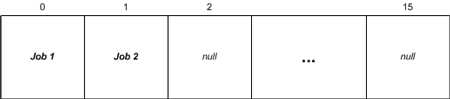
\includegraphics[scale=0.75]{ArrayList-1}
\caption{The ArrayList after the first two lines of code}
\label{ArrayList-1}
\end{center}
\end{figure}
Note that there are 16 elements in the ArrayList at this point because, by default, the ArrayList, when initialized, creates its internal object array with 16 elements. Next, the GetNextJob() method is invoked, which removes the first job, resulting in something like Figure \ref{ArrayList-2} presented in page \pageref{ArrayList-2}.
\begin{figure}
\begin{center}
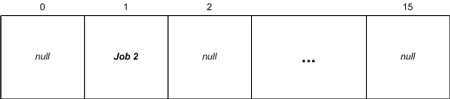
\includegraphics[scale=0.75]{ArrayList-2}
\caption{Program after the GetNextJob() method is invoked}
\label{ArrayList-2}
\end{center}
\end{figure}
When AddJob("3") executes, we need to add another job to the buffer. Clearly the first ArrayList element (index 0) is available for reuse. Initially it might make sense to put the third job in the 0 index. However, this approach can be forgotten by considering what would happen if after AddJob("3") we did AddJob("4"), followed by two calls to GetNextJob(). If we placed the third job in the 0 index and then the fourth job in the 2 index, we'd have the problem demonstrated in Figure \ref{ArrayList-3} presented in page \pageref{ArrayList-3}.
\begin{figure}
\begin{center}
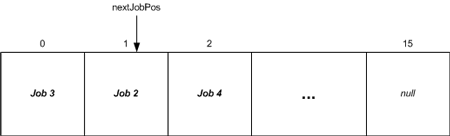
\includegraphics[scale=0.75]{ArrayList-3}
\caption{Issue Created by placing jobs in the 0 index}
\label{ArrayList-3}
\end{center}
\end{figure}
Now, when GetNextJob() was called, the second job would be removed from the buffer, and nextJobPos would be incremented to point to index 2. Therefore, when GetNextJob() was called again, the fourth job would be removed and processed prior to the third job, thereby violating the first come, first served order we need to maintain. The crux of this problem arises because the ArrayList represents the list of jobs in a linear ordering. That is, we need to keep adding the new jobs to the right of the old jobs to guarantee that the correct processing order is maintained. Whenever we hit the end of the ArrayList, the ArrayList is doubled, even if there are unused ArrayList elements due to calls to GetNextJob(). To fix this problem, we need to make our ArrayList circular. A circular array is one that has no definite start or end. Rather, we have to use variables to maintain the beginning and end of the array. A graphical representation of a circular array is shown in Figure \ref{CircularArray} presented in page \pageref{CircularArray}.
\begin{figure}
\begin{center}
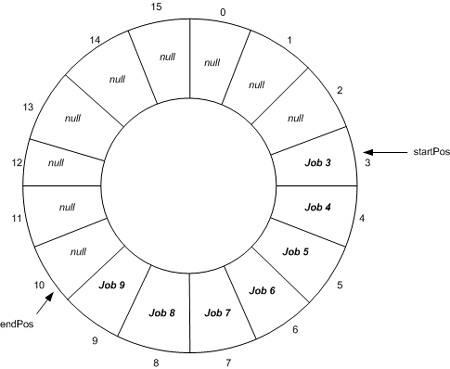
\includegraphics[scale=0.75]{CircularArray}
\caption{Example of a Circular Array}
\label{CircularArray}
\end{center}
\end{figure}
With a circular array, the AddJob() method adds the new job in index endPos and then "increments" endPos. The GetNextJob() method plucks the job from startPos, sets the element at the startPos index to null, and "increments" startPos. I put the word increments in quotation marks because here incrementing is a trifle more complex than simply adding one to the variable's current value. To see why we can't just add 1, consider the case when endPos equals 15. If we increment endPos by adding 1, endPos equals 16. In the next AddJob() call, the index 16 will attempt to be accessed, which will result in an IndexOutOfRangeException. Rather, when endPos equals 15, we want to increment endPos by resetting it to 0. This can either be done by creating an increment(variable) function that checks to see if the passed-in variable equals the array's size and, if so, reset it to 0. Alternatively, the variable can have its value incremented by 1 and then moded by the size of the array. In such a case, the code for increment() would look like:
\begin{lstlisting}
int increment(int variable)
{
  return (variable + 1) % theArray.Length;
}
\end{lstlisting}
The modulus operator, \%, when used like x\% y, calculates the remainder of x divided by y. The remainder is always between 0 and y – 1. This approach works well if our buffer never has more than 16 elements, but what happens if we want to add a new job to the buffer when there are already 16 jobs present? Like with the ArrayList's Add() method, we'll need to redimension the circular array appropriately, by, say, doubling the size of the array.
\subsection{Queue Operations}
The two primary operations involving queues are adding a new item to the queue and removing an item from the queue. The operation for adding a new item is called Enqueue, and the operation for removing an item from a queue is called Dequeue. The Enqueue operation adds an item at the end of the queue and the Dequeue operation removes an item from the front (or beginning) of the queue. Figure \ref{QueueOperations-} presented in page \pageref{QueueOperations-}  illustrates these operations.
The other primary operation to perform on a queue is viewing the beginning item. The Peek method, like its counterpoint in the Stack class, is used to view the beginning item. This method simply returns the item without actually removing it from the queue.
There are other properties of the Queue class we can use to aid in our programming. However, before we discuss them let’s look at how we can implement a Queue class.
\begin{figure}
\begin{center}
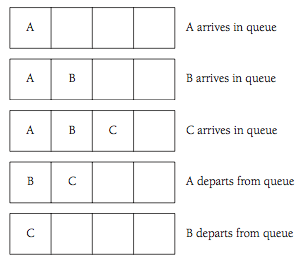
\includegraphics[scale=0.75]{QueueOperations-}
\label{QueueOperations-}
\caption{Queue Operations}
\end{center}
\end{figure}
\subsection{Building Our Own Queue}
Implementing the Queue class using an ArrayList is practically a no-brainer, as was our implementation of the Stack class. ArrayLists are excellent implementation choices for these types of data structures because of their built-in dynamics. When we need to insert an item into our queue, the Arraylist Add method places the item in the next free element of the list. When we need to remove the front item from the queue, the ArrayList moves each remaining item in the list up one element. We don’t have to maintain a placeholder, which can lead to subtle errors in your code.
The following Queue class implementation includes methods for EnQueue, DeQueue, ClearQueue (clearing the queue), Peek, and Count, as well as a default constructor for the class:
\begin{lstlisting}
public class CQueue{
	private ArrayList pqueue; 
	public CQueue(){
		pqueue = new ArrayList();
	}
	public void EnQueue(object item){
		pqueue.Add(item);
	}
	public void DeQueue( ) {
		pqueue.RemoveAt(0);
	}
	public object Peek( ) {
		return pqueue[0];
	}
	public void ClearQueue( ) {
		pqueue.Clear();
	}
	public int Count( ) {
		return pqueue.Count;
	}
}
\end{lstlisting}
\subsection{Sorting Data wih Queues}
Back in the old days of computing, programs were entered into a mainframe computer via punch cards, where each card held a single program statement. Cards were sorted using a mechanical sorter that utilized bin-like structures. We can simulate this process by sorting data using queues. This sorting technique is called a radix sort. It will not be the fastest sort in your programming repertoire, but the radix sort does demonstrate another interesting use of queues.
The radix sort works by making two passes over a set of data, in this case integers in the range 0–99. The first pass sorts the numbers based on the 1’s digit and the second pass sorts the numbers based on the 10’s digit. Each number is then placed in a bin based on the digit in each of these places. Given these numbers:\\
\texttt{91 46 85 15 92 35 31 22}\\
The first pass results in this bin configuration:
\textbf{
\\Bin 0:
\\Bin 1: 91 31 
\\Bin 2: 92 22 
\\Bin 3:
\\Bin 4:
\\Bin 5: 85 15 35 
\\Bin 6: 46
\\Bin 7:
\\Bin 8:
\\Bin 9:}
Now put the numbers in order based on which bin they’re in:\\
\texttt{91 31 92 22 85 15 35 46}
\\Next, take the list and sort by the 10’s digit into the appropriate bins:
\textbf{
\\Bin 0:
\\Bin 1: 15 
\\Bin 2: 22 
\\Bin 3: 31 35 
\\Bin 4: 46 
\\Bin 5:
\\Bin 6:
\\Bin 7:
\\Bin 8: 85 
\\Bin 9: 91 92}
Take the numbers from the bins and put them back into a list, which results in a sorted set of integers:\\
\texttt{15 22 31 35 46 85 91 92}\\
We can implement this algorithm by using queues to represent the bins. We need nine queues, one for each digit. We use modulus and integer division for determining the 1’s and 10’s digits. The rest is a matter of adding numbers to their appropriate queues, taking them out of the queues to resort based on the 1’s digit, and then repeating the process for the 10’s digit. The result is a sorted list of integers.
Here’s the code:
\begin{lstlisting}
using System;
using System.Collections;
using System.IO;
namespace csqueue{
	class Class1{
		enum DigitType {ones = 1, tens = 10}
		static void DisplayArray(int [] n){
			for(int x = 0; x <= n.GetUpperBound(0); x++)
  				Console.Write(n[x] + " ");
  		}
		static void RSort(Queue[] que, int[] n, DigitType digit){
			int snum;
			for(int x = 0; x <= n.GetUpperBound(0); x++){
				if (digit == DigitType.ones)
					snum = n[x] % 10;
				else
					snum = n[x] / 10;
				que[snum].Enqueue(n[x]);
			}
		}
	static void BuildArray(Queue[] que, int[] n){
		int y = 0;
		for(int x = 0; x >= 9; x++)
   			while(que[x].Count > 0){
   				n[y] = Int32.Parse(que[x].Dequeue().ToString());
   				y++;
   			}
   	}
	static void Main(string[] args){
		Queue [] numQueue = new Queue[10];
		int [] nums = new int[] {91, 46, 85, 15, 92, 35, 31, 22}; 
		int[] random = new Int32[99];
		// Display original list
		for(int i = 0; i < 10; i++)
   			numQueue[i] = new Queue();
		RSort(numQueue, nums, DigitType.ones);
		//numQueue, nums, 1
		BuildArray(numQueue, nums);
		Console.WriteLine();
		Console.WriteLine("First pass results: ");
		DisplayArray(nums);
		// Second pass sort
		RSort(numQueue, nums, DigitType.tens);
		BuildArray(numQueue, nums);
		Console.WriteLine();
		Console.WriteLine("Second pass results: ");
		// Display final results
		DisplayArray(nums);
		Console.WriteLine();
		Console.Write("Press enter to quit");
        Console.Read();
        }
    }
}
\end{lstlisting}
The RSort subroutine is passed the array of queues, the number array, and a descriptor telling the subroutine whether to sort the 1’s digit or the 10’s digit. If the sort is on the 1’s digit, the program calculates the digit by taking the remainder of the number modulus 10. If the sort is on the 10’s digit, the program calculates the digit by taking the number and dividing (in an integer-based manner) by 10.
To rebuild the list of numbers, each queue is emptied by performing successive Dequeue operations while there are items in the queue. This is performed in the BuildArray subroutine. Since we start with the array that is holding the smallest numbers, the number list is built “in order.”
\subsection{Priority Queues}
Queue is a data structure where the first item placed in the structure is the first item taken out of the structure. The effect of the behavior is the oldest item in the structure that is removed first. For many applications, though, a data structure is needed where an item with the highest priority is removed first, even if it isn’t the “oldest” item in the structure. There is a special case of the Queue made for this type of application—the priority queue.
There are many applications that utilize priority queues in their operations. A good example is process handling in a computer operating system. Certain processes have a higher priority than other processes, such as printing pro- cesses, which typically have a low priority. Processes (or tasks) are usually numbered by their priority, with a Priority 0 process having a higher priority than a Priority 20 task. Items stored in a priority queue are normally constructed as key–value pairs, where the key is the priority level and the value identifies the item. For example, an operating system process might be defined like this:
\begin{lstlisting}
struct Process { 
	int priority; 
	string name;
}
\end{lstlisting}
We cannot use an unmodified Queue object for a priority queue. The DeQueue method simply removes the first item in the queue when it is called. We can, though, derive our own priority queue class from the Queue class, overriding Dequeue to make it do our bidding. We’ll call the class PQueue. We can use all of the Queue methods as is, and override the Dequeue method to remove the item that has the high- est priority. To remove an item from a queue that is not at the front of the queue, we have to first write the queue items to an array. Then we can iterate through the array to find the highest priority item. Finally, with that item marked, we can rebuild the queue, leaving out the marked item. Here’s the code for the PQueue class:
\begin{lstlisting}
public struct pqItem { 
	public int priority; 
	public string name;
}
public class PQueue : Queue {
	public PQueue { 
		base();
}
public override object Dequeue() {
      object [] items;
      int x, min, minindex;
      items = this.ToArray();
      min = (pqItem)items[0].priority;
      for(int x = 1; x <= items.GetUpperbound(0); x++)
      	if ((pqItem)items[x].Priority < min) { 
      		min = (pqItem)items[x].Priority; minindex = x;
		}
     this.Clear();
     for(int x = 0; x <= items.GetUpperBound(0); x++)
       if (x != minindex && (pqItem)items[x].name != "")
          this.Enqueue(items[x]);
     return items[minindex];
	}
}
\end{lstlisting}
The following code demonstrates a simple use of the PQueue class. An emergency waiting room assigns a priority to patients who come in for treatment. A patient presenting symptoms of a heart attack is going to be treated before a patient who has a bad cut. The following program simulates three patients entering an emergency room at approximately the same time. Each patient is seen by the triage nurse, assigned a priority, and added to the queue. The first patient to be treated is the patient removed from the queue by the Dequeue method.
\begin{lstlisting}
static void Main() {
	PQueue erwait = new PQueue();
	pqItem[] erPatient = new pqItem[4];
	pqItem nextPatient;
	erPatient[0].name = "Joe Smith"; erPatient[0].priority = 1;
	erPatient[1].name = "Mary Brown"; erPatient[1].priority = 0;
	erPatient[2].name = "Sam Jones"; erPatient[2].priority = 3;
	for(int x = 0; x <= erPatient.GetUpperbound(0); x++)
      erwait.Enqueue(erPatient[x]);
    nextPatient = erwait.Dequeue();
    Console.WriteLine(nextPatient.name);
}
\end{lstlisting}
The output of this program is “Mary Brown”, since she has a higher priority than the other patients.
\section{Summary}
Learning to use data structures appropriately and efficiently is one of the skills that separates the expert programmer from the average programmer. The expert programmer recognizes that organizing a program’s data into an appropriate data structure makes it easier to work with the data. In fact, thinking through a computer programming problem using data abstraction makes it easier to come up with a good solution to the problem in the first place.
We discussed using two very common data structures in this chapter: the stack and the queue. Stacks are used for solving many different types of problems in computer programming, especially in systems’ programming areas such as interpreters and compilers. We also saw how we can use stacks to solve more generic problems, such as determining if a word is a palindrome.
Queues also have many applications. Operating systems use queues for ordering processes (via priority queues) and queues are used quite often for simulating real world processes. Finally, we used the Queue class to derive a class for implementing a priority queue. The ability to derive new classes from classes in the .NET Framework class library is one of the major strengths of the .NET version of C\#.
\section{Labs}
\begin{enumerate}
\item You can use a Stack to check if a programming statement or a formula has balanced parentheses. Write a Windows application that provides a text box for the user to enter an expression with parenthesis. Provide a Check Parens button that, when clicked, runs a program that checks the number of parentheses in the expression and highlights a parenthesis that is unbalanced.
\item A postfix expression evaluator works on arithmetic statements that take this form: op1 op2 operator . . . Using two stacks, one for the operands and one for the operators, design and implement a Calculator class that converts infix expressions to postfix expressions and then uses the stacks to evaluate the expressions.
\item This exercise involves designing a help-desk priority manager. Help requests are stored in a text file with the following structure: priority, id of requesting party, time of request The priority is an integer in the range 1–5 with 1 being the least important and 5 being the most important. The id is a four-digit employee identification number and the time is in TimeSpan.Hours, TimeSpan.Minutes, TimeSpan.Seconds format. Write a Windows application that, during the Form Load event, reads five records from the data file containing help requests, prioritizes the list using a priority queue, and displays the list in a list box. Each time a job is completed, the user can click on the job in the list box to remove it. When all five jobs are completed, the application should automatically read five more data records, prioritize them, and display them in the list box.
\end{enumerate}

\chapter{String Class, String Builder, and Pattern Matching}
Strings are common to most computer programs. Certain types of programs, such as word processors and web applications, make heavy use of strings, which forces the programmer of such applications to pay special attention to the efficiency of string processing. In this chapter, we examine how C\# works with strings, how to use the String class, and finally, how to work with the StringBuilder class. The StringBuilder class is used when a program must make many changes to a String object because strings and String objects are immutable, whereas StringBuilder objects are mutable.
\section{String Class}
A string is a series of characters that can include letters, numbers, and other symbols. String literals are created in C\# by enclosing a series of characters within a set of double quotation marks. Here are some examples of string literals:
\begin{lstlisting}
"Haitham El-Ghareeb"
"the quick brown fox jumped over the lazy dog"
"123-45-6789"
"helghareeb@mans.edu.eg"
\end{lstlisting}
A string can consist of any character that is part of the Unicode character set. A string can also consist of no characters. This is a special string called the empty string and it is shown by placing two double quotation marks next to each other (“ ”). Please keep in mind that this is not the string that represents a space. That string looks like this—“ ”.
Strings in C\# have a special nature—they are both native types and objects of a class. Actually, to be more precise, we should say that we can work with strings as if they are native data values, but in reality every string created is an object of String class.
\subsection{Creating String Object}
Strings are created like this:
\begin{lstlisting}
string name = "Haitham A. El-Ghareeb";
\end{lstlisting}
though you can of course, declare the variable and assign it data in two separate statements. The declaration syntax makes name look like it is just a regular variable, but it is actually an instance of a String object.
C\# strings also allow you to place escape characters inside the strings. Escape characters are used to place format characters such as line breaks and tab stops within a string.
\subsection{String Class Methods}
Although there are many operations we can perform on strings, a small set of operations dominates. Three of the top operations are as follows: 
\begin{enumerate}
\item finding a substring in a string
\item determining the length of a string, and 
\item determining the position of a character in a string.
\end{enumerate}
The following short program demonstrates how to perform these operations. A String object is instantiated to the string “Haitham El-Ghareeb”. We then break the string into its two constituent pieces: the first word and the second word. Here’s the code, followed by an explanation of the String methods used:
\begin{lstlisting}
using System;
class MyStringExample
{
	static void Main() {
	string string1 = "Haitham, El-Ghareeb!";
	int len = string1.Length;
	int pos = string1.IndexOf(" "); 
	string firstWord, secondWord; 
	firstWord = string1.Substring(0, pos); 
	secondWord = string1.Substring(pos+1, (len-1)-(pos+1));
  	Console.WriteLine("First word: " + firstWord);
  	Console.WriteLine("Second word: " + secondWord);
  	Console.Read();
	} 
}
\end{lstlisting}
The first thing we do is use Length property to determine the length of the object string. The length is simply the total number of all the characters in the string. To break up a two-word phrase into separate words, we need to know what separates the words. In a well-formed phrase, a space separates words and so we want to find the space between the two words in this phrase. We can do this with the IndexOf method. This method takes a character and returns the character’s position in the string. Strings in C\# are zero-based and therefore the first character in the string is at position 0, the second character is at position 1, and so on. If the character can’t be found in the string, a-1 is returned. The IndexOf method finds the position of the space separating the two words and is used in the next method, Substring, to actually pull the first word out of the string. The Substring method takes two arguments: a starting position and the number of characters to pull. Look at the following example:
\begin{lstlisting}
string m = "Now is the time";
string sub = m.Substring(0,3);
\end{lstlisting}
The value of sub is “Now”. The Substring method will pull as many characters out of a string as you ask it to, but if you try to go beyond the end of the string, an exception is thrown. The first word is pulled out of the string by starting at position 0 and pulling out pos number of characters. This may seem odd, since pos contains the position of the space, but because strings are zero-based, this is the correct number.
The next step is to pull out the second word. Since we know where the space is, we know that the second word starts at pos+1 (again, we’re assuming we’re working with a well-formed phrase where each word is separated by exactly one space). The harder part is deciding exactly how many characters to pull out, knowing that an exception will be thrown if we try to go beyond the end of the string. There is a formula of sorts we can use for this calculation. First, we add 1 to the position where the space was found and then subtract that value from the length of the string. That will tell the method exactly how many characters to extract.
Although this short program is interesting, it’s not very useful. What we really need is a program that will pull out the words out of a well-formed phrase of any length. There are several different algorithms we can use to do this.
The algorithm we’ll use here contains the following steps:
\begin{enumerate}
\item Find the position of the first space in the string.
\item Extract the word.
\item Build a new string starting at the position past the space and continuing until the end of the string.
\item Look for another space in the new string.
\item If there isn’t another space, extract the word from that position to the end of the string.
\item Otherwise, loop back to step 2.
\end{enumerate}
Here is the code we built from this algorithm (each word extracted from the string is stored in a collection named words):
\begin{lstlisting}
using System; 
class separateWords {
	static void Main() {
		string astring = "I love String Manipulation"; 
		int pos;
		string word;
		ArrayList words = new ArrayList(); 
		pos = astring.IndexOf(" ");
		While (pos > 0) {
        	word = astring.Substring(0,pos);
        	words.Add(word);
        	astring = astring.Substring(pos+1, astring.Length - (pos + 1)); pos = astring.IndexOf(" ");
		if (pos == -1) {
			word = astring.Substring(0, asstring.Length); words.Add(word);
		}
      Console.Read();
      }
	}
}
\end{lstlisting}
Of course, if we were going to actually use this algorithm in a program we’d make it a function and have it return a collection, like this:
\begin{lstlisting}
using System;
using System.Collections;
class StringManipulation {
	static void Main() {
		string astring = "I still Love String Manipulation";
      	ArrayList words = new ArrayList();
      	words = SplitWords(astring);
      	foreach (string word in words)
        	Console.Write(word + " ");
      		Console.Read();
	}
	static ArrayList SplitWords(string astring) { 
		string[] ws = new string[astring.Length-1]; 
		ArrayList words = new ArrayList();
		int pos;
		string word;
		pos = astring.IndexOf(" "); 
		while (pos > 0) {
	        word = astring.Substring(0, pos);
    	    words.Add(word);
        	astring = astring.Substring(pos+1, astring.Length-(pos+1)); 
        	if (pos == -1) {
	          word = astring.Substring(0, astring.Length);
    	      words.Add(word);
			}
		}
      return words;
	}
}
\end{lstlisting}
It turns out, though, that the String class already has a method for splitting a string into parts (the Split method) as well as a method that can take a data collection and combine its parts into a string (the Join method).
\subsection{Join and Split Methods}
Breaking up strings into individual pieces of data is a very common function. Many programs, from Web applications to everyday office applications, store data in some type of string format. To simplify the process of breaking up strings and putting them back together, the String class provides two methods to use: the Split method for breaking up strings and the Join method for making a string out of the data stored in an array. The Split method takes a string, breaks it into constituent pieces, and puts those pieces into a String array. The method works by focusing on a separating character to determine where to break up the string. In the example in the last section, the SplitWords function always used the space as the separator. We can specify what separator to look for when using the Split method. In fact, the separator is the first argument to the method. The argument must come in the form of a char array, with the first element of the array being the character used as the delimiter.
Many application programs export data by writing out strings of data separated by commas. These are called comma-separated value strings or CSVs for short. Some authors use the term comma-delimited. A comma-delimited string looks like this:\\
\texttt{"Haitham, El-Ghareeb, Information Systems Department, Faculty of Computers and Information Sciences, Mansoura University, Egypt,35516”}\\
Each logical piece of data in this string is separated by a comma. We can put each of these logical pieces into an array using the Split method like this:
\begin{lstlisting}
string data = "Haitham, El-Ghareeb, Information Systems Department, Faculty of Computers and Information Sciences, Mansoura University, Egypt,35516";
string[] sdata;
char[] delimiter = new char[] {','};
sdata = data.Split(delimiter, data.Length);
\end{lstlisting}
Now we can access this data using standard array techniques:
\begin{lstlisting}
foreach (string word in sdata)
    Console.Write(word + " ");
\end{lstlisting}
There is one more parameter we can pass to the Split method—the number of elements we want to store in the array. For example, if I want to put the first string element in the first position of the array and the rest of the string in the second element, I would call the method like this:
\begin{lstlisting}
sdata = data.Split(delimiter,2);
\end{lstlisting}
The elements in the array are:
\begin{itemize}
\item 0th element-Haitham
\item 1st element-El-Ghareeb, Information Systems Department, Faculty of Computers and Information Sciences, Mansoura University, Egypt,35516
\end{itemize}
We can go the other way, from an array to a string, using the Join method. This method takes two arguments:the original array and a character to separate the elements. A string is built consisting of each array element followed by the separator element. We should also mention that this method is often called as a class method, meaning we call the method from the String class itself and not from a String instance.\\
Here’s an example using the same data we used for the Split method:
\begin{lstlisting}
using System; 
class JoinString {
	static void Main() {
		string data = "Haitham, El-Ghareeb, Information Systems Department, Faculty of Computers and Information Sciences, Mansoura University, Egypt,35516";
      	string[] sdata;
		char[] delimiter = new char[] {','};
		sdata = data.Split(delimiter, data.Length); 
		foreach (string word in sdata)
        	Console.Write(word + " ");
      	string joined;
      	joined = String.Join(',', sdata);
      	Console.Write(joined);
	} 
}
\end{lstlisting}
These methods are useful for getting data into your program from another source (the Split method) and sending data out of your program to another source (the Join method).
\subsection{Comparing Strings}
There are several ways to compare String objects in C\#. The most obvious ways are to use the relational operators, which for most situations will work just fine. However, there are situations where other comparison techniques are more useful, such as if we want to know if a string is greater than, less than, or equal to another string, and for situations like that we have to use methods found in the String class. Strings are compared with each other much as we compare numbers. However, since it’s not obvious if “a” is greater than or less than “H”, we have to have some sort of numeric scale to use. That scale is the Unicode table. Each character (actually every symbol) has a Unicode value, which the operating system uses to convert a character’s binary representation to that character. You can determine a character’s Unicode value by using the ASC function. ASC actually refers to the ASCII code of a number. ASCII is an older numeric code that precedes Unicode, and the ASC function was first developed before Unicode subsumed ASCII.
To find the ASCII value for a character, simply convert the character to an integer using a cast, like this:
\begin{lstlisting}
int charCode;
charCode = (int)'a';
\end{lstlisting}
The value 97 is stored in the variable.\\
Two strings are compared, then, by actually comparing their numeric codes. The strings “a” and “b” are not equal because code 97 is not code 98. The compareTo method actually lets us determine the exact relationship between two String objects. We’ll see how to use that method shortly. The first comparison method we’ll examine is the Equals method. This method is called from a String object and takes another String object as its argument. It then compares the two String objects character-by-character. If they contain the same characters (based on their numeric codes), the method returns True. Otherwise, the method returns False. The method is called like this:
\begin{lstlisting}
string s1 = "Haitham";
string s2 = "Haitham";
if (s1.Equals(s2))
	Console.WriteLine("They are the same.");
else
	Console.WriteLine("They are not the same.");
\end{lstlisting}
The next method for comparing strings is CompareTo. This method also takes a String as an argument but it doesn’t return a Boolean value. Instead, the method returns either 1, -1, or 0, depending on the relationship between he passed-in string and the string instance calling the method. Here are some examples:
\begin{lstlisting}
string s1 = "Haitham";
string s2 = "Haitham";
Console.WriteLine(s1.CompareTo(s2)); // returns 0
s2 = "foofoo";
Console.WriteLine(s1.CompareTo(s2)); // returns -1
s2 = "fooaar";
Console.WriteLine(s1.CompareTo(s2)); // returns 1
\end{lstlisting}
If two strings are equal, the CompareTo method returns a 0; if the passed-in string is “below” the method-calling string, the method returns a -1; if the passed-in string is “above” the method-calling string, the method returns a 1.
An alternative to the CompareTo method is the Compare method, which is usually called as a class method. This method performs the same type of comparison as the CompareTo method and returns the same values for the same comparisons. The Compare method is used like this:
\begin{lstlisting}
static void Main() {
	string s1 = "Haitham";
	string s2 = "Haitham";
	int compVal = String.Compare(s1, s2); 
	switch(compVal) {
      case 0 : 
      	Console.WriteLine(s1 + " " + s2 + " are equal");
      	break;
     case 1 : 
     	Console.WriteLine(s1 + " is less than " + s2);
     	break;
     case 2 : 
     	Console.WriteLine(s1 + " is greater than" + s2);
        break;
      default : Console.WriteLine("Can't compare");
	}
}
\end{lstlisting}
Two other comparison methods that can be useful when working with strings are StartsWith and EndsWith. These instance methods take a string as an argument and return True if the instance either starts with or ends with the string argument.
Following are two short programs that demonstrate the use of these methods. First, we’ll demonstrate the EndsWith method:
\begin{lstlisting}
using System;
using System.Collections;
class StringComparison {
	static void Main() {
	string[] nouns = new string[] {"apples", "oranges", "banana", "cherry", "tomatoes"}; 
	ArrayList pluralNouns = new ArrayList();
	foreach (string noun in nouns)
		if (noun.EndsWith("s"))
            pluralNouns.Add(noun);
      foreach (string noun in pluralNouns)
        Console.Write(noun + " ");
	}
}
\end{lstlisting}
First, we create an array of nouns, some of which are in plural form. Then we loop through the elements of the array, checking to see if any of the nouns are plurals. If so, they’re added to a collection. Then we loop through the collection, displaying each plural.

We use the same basic idea in the next program to determine which words start with the prefix “tri”:
\begin{lstlisting}
using System;
using System.Collections;
class StringEndings {
static void Main() {
	string[] words = new string[] {"triangle", "diagonal", "trimester","bifocal", "triglycerides"};
	ArrayList triWords = new ArrayList();
	foreach (string word in words)
  		if (word.StartsWith("tri"))
     		triWords.Add(word);
	foreach (string word in triWords)
  		Console.Write(word + " ");
	}
}
\end{lstlisting}
\subsection{String Manipulation}
String processing usually involves making changes to strings. We need to insert new characters into a string, remove characters that don’t belong anymore, replace old characters with new characters, change the case of certain characters, and add or remove space from strings, just to name a few operations. There are methods in the String class for all of these operations, and in this section we’ll examine them. We’ll start with the Insert method. This method inserts a string into another string at a specified position. Insert returns a new string. The method is called like this:
\begin{lstlisting}
String1 = String0.Insert(Position, String)
\end{lstlisting}
An example of using this code is:
\begin{lstlisting}
using System; 
class StringManipulation {
	static void Main() {
	string s1 = "Hello, . Welcome to Data Structures and Algorithms class."; 
	string name = "Ahmed";
	int pos = s1.IndexOf(",");
	s1 = s1.Insert(pos+2, name); 
	Console.WriteLine(s1);
	} 
}
\end{lstlisting}
The output is
\texttt{Hello, Ahmed. Welcome to Data Structures and Algorithms class.}\\
The program creates a string, s1, which deliberately leaves space for a name, much like you’d do with a letter you plan to run through a mail merge. We add two to the position where we find the comma to make sure there is a space between the comma and the name. The next most logical method after Insert is Remove. This method takes two Integer arguments: a starting position and a count, which is the number of characters you want to remove. Here’s the code that removes a name from a string after the name has been inserted:
\begin{lstlisting}
using System; 
class StringManipulation {
	static void Main() {
		string s1 = "Hello, . Welcome to Data Structures and Algorithms class."; 
		string name = "Saed";
		int pos = s1.IndexOf(",");
		s1 = s1.Insert(pos+2, name); 
		Console.WriteLine(s1);
		s1 = s1.Remove(pos+2, name.Length); 
		Console.WriteLine(s1);
	}
}
\end{lstlisting}
The Remove method uses the same position for inserting a name to remove the name, and the count is calculated by taking the length of the name variable. This allows us to remove any name inserted into the string. The next logical method is the Replace method. This method takes two arguments: a string of characters to remove and a string of characters to replace them with. The method returns the new string. Here’s how to use Replace:
\begin{lstlisting}
using System; 
class StringManipulation {
	static void Main() {
		string[] words = new string[] {"recieve", "decieve", "reciept"};
		for(int i = 0; i <= words.GetUpperBound(0); i++) {
			words[i] = words[i].Replace("cie", "cei");
			Console.WriteLine(words[i]);
		} 
	}
}
\end{lstlisting}
The only tricky part of this code is the way the Replace method is called. Since we’re accessing each String object via an array element, we have to use array addressing followed by the method name, causing us to write this fragment:
\begin{lstlisting}
words(index).Replace("cie", "cei");
\end{lstlisting}
There is no problem with doing this, of course, because the compiler knows that words(index) evaluates to a String object.  When displaying data from our programs, we often want to align the data within a printing field in order to line the data up nicely. The String class includes two methods for performing this alignment: PadLeft and PadRight. The PadLeft method right-aligns a string and the PadRight method left-aligns a string. For example, if you want to print the word “Hello” in a 10-character field right-aligned, you would write this:
\begin{lstlisting}
string s1 = "Hello";
Console.WriteLine(s1.PadLeft(10));
Console.WriteLine("world");
\end{lstlisting}
The output is:
\begin{lstlisting}
	Hello 
world
\end{lstlisting}
Here’s an example using PadRight:
\begin{lstlisting}
string s1 = "Haitham";
string s2 = "Abdel Monem";
string s3 = "El-Ghareeb";
Console.Write(s1.PadLeft(10));
Console.WriteLine(s2.PadLeft(10));
Console.Write(s3.PadLeft(10));
Console.WriteLine(s2.Padleft(10));
\end{lstlisting}
We end this section with a discussion of the Trim and TrimEnd methods. When working with String objects, they sometimes have extra spaces or other formatting characters at the beginning or at the end of the string. The Trim and TrimEnd methods will remove spaces or other characters from either end of a string. You can specify either a single character to trim or an array of characters. If you specify an array of characters, if any of the characters in the array are found, they will be trimmed from the string. Let’s first look at an example that trims spaces from the beginning and end of a set of string values:
\begin{lstlisting}
using System; 
class StringManipulation {
	static void Main() {
		string[] names = new string[] {" Haitham ", " Mohamed ", "Ahmed ", " Saed"};
	Console.WriteLine();
	showNames(names);
	Console.WriteLine();
	trimVals(names);
	Console.WriteLine();
    showNames(names);
	}
	static void showNames(string[] arr) {
      for(int i = 0; i <= arr.GetUpperBound(0); i++)
        Console.Write(arr[i]);    
	}
	static void trimVals(string[] arr) {
		char[] charArr = new char[] {' '};
		for(int i = 0; i<= arr.GetUpperBound(0); i++) {
    		arr[i] = arr[i].Trim(charArr[0]);
    		arr[i] = arr[i].TrimEnd(charArr[0]);
    	}
    }
}
\end{lstlisting}
\section{String Builder}
The StringBuilder class provides access to mutable String objects. Objects of the String class are immutable, meaning that they cannot be changed. Every time you change the value of a String object, a new object is created to hold the value. StringBuilder objects, on the other hand, are mutable. When you make a change to a StringBuilder object, you are changing the original object, not working with a copy. In this section, we discuss how to use the StringBuilder class for those situations where many changes are to be to the String objects in your programs. The StringBuilder class is found in the System.Text namespace so you must import this namespace into your program before you can use StringBuilder objects.
You can construct a StringBuilder object in one of three ways. The first way is to create the object using the default constructor:
\begin{lstlisting}
StringBuilder stBuff1 = new StringBuilder();
\end{lstlisting}
This line creates the object stBuff1 with the capacity to hold a string 16 characters in length. This capacity is assigned by default, but it can be changed by passing in a new capacity in a constructor call, like this:
\begin{lstlisting}
StringBuilder stBuff2 = New StringBuilder(25);
\end{lstlisting}
This line builds an object that can initially hold 25 characters. The final constructor call takes a string as the argument:
\begin{lstlisting}
StringBuilder stBuff3 = New StringBuilder("Hello, world");
\end{lstlisting}
The capacity is set to 16 because the string argument didn’t exceed 16 characters. Had the string argument been longer than 16, the capacity would have been set to 32. Every time the capacity of a StringBuilder object is exceeded, the capacity is increased by 16 characters.
There are several properties in the StringBuilder class that you can use to obtain information about a StringBuilder object. The Length property specifies the number of characters in the current instance and the Capacity property returns the current capacity of the instance. The MaxCapacity property returns the maximum number of characters allowed in the current instance of the object (though this is automatically increased if more characters are added to the object).
The following program fragment demonstrates how to use these properties:
\begin{lstlisting}
StringBuilder stBuff = new StringBuilder("Haitham El-Ghareeb");
Console.WriteLine("Length of stBuff3: " & stBuff.Length());
Console.WriteLine("Capacity of stBuff3: " & stBuff.Capacity());
Console.WriteLine("Maximum capacity of stBuff3: " + stBuff.MaxCapacity);
\end{lstlisting}
The Length property can also be used to set the current length of a String- Builder object, as in
\begin{lstlisting}
stBuff.Length = 10;
Console.Write(stBuff3);
\end{lstlisting}
This code outputs “Haitham El".
To ensure that a minimum capacity is maintained for a StringBuilder instance, you can call the EnsureCapacity method, passing in an integer that states the minimum capacity for the object. Here’s an example:
\begin{lstlisting}
stBuff.EnsureCapacity(25);
\end{lstlisting}
Another property you can use is the Chars property. This property either returns the character in the position specified in its argument or sets the character passed as an argument. The following code shows a simple example using the Chars property.
\begin{lstlisting}
StringBuilder stBuff = New StringBuilder("Haitham El-Ghareeb");
If (stBuff.Chars(0) <> "D")
	stBuff.Chars(0) = "D";
\end{lstlisting}
\subsection{Modifying StringBuilder Objects}
We can modify a StringBuilder object by appending new characters to the end of the object, inserting characters into an object, replacing a set of characters in an object with different characters, and remove characters from an object. You can add characters to the end of a StringBuilder object by using the Append method. This method takes a string value as an argument and concatenates the string to the end of the current value in the object. The following program demonstrates how the Append method works:
\begin{lstlisting}
Using System.Text; 
class StringBuilderManipulation {
	static void Main() {
		StringBuilder stBuff As New StringBuilder(); 
		String[] words = new string[] {"now ", "is ", "the ", "time ", "for ", "all ", "good ", "men ", "to ", "come ", "to ", "the ", "aid ", "of ", "their ", "party"}
      For(int i = 0; i <= words.GetUpperBound(0); i++)
      	stBuff.Append(words(index));
      Console.WriteLine(stBuff);
	}
}
\end{lstlisting}
The output is, of course\\
Now is the time for all good men to come to the aid of their party\\
A formatted string can be appended to a StringBuilder object. A formatted string is a string that includes a format specification embedded in the string. There are too many format specifications to cover in this section, so we’ll just demonstrate a common specification. We can place a formatted number within a StringBuilder object like this:
\begin{lstlisting}
Using System.Text; 
class StringBuilderManipulation {
	static void Main() {
		StringBuilder stBuff = New StringBuilder(); 
		Console.WriteLine(); 
		stBuff.AppendFormat("Your order is for {0000} widgets.", 234);
		stBuff.AppendFormat("\nWe have {0000} widgets left.", 12);
		Console.WriteLine(stBuff);
	}
}
\end{lstlisting}
The format specification is enclosed within curly braces that are embedded in a string literal. The data after the comma is placed into the specification when the code is executed.\\ 
Next is the Insert method. This method allows us to insert a string into the current StringBuilder object. The method can take up to three arguments. The first argument specifies the position to begin the insertion. The second argu- ment is the string you want to insert. The third argument, which is optional, is an integer that specifies the number of times you want to insert the string into the object. Here’s a small program that demonstrates how the Insert method is used:
\begin{lstlisting}
Using System.Text; 
class StringBuilderManipulation {
	static void Main(){
		StringBuilder stBuff = New StringBuilder(); 
		stBuff.Insert(0, "Hello");
		stBuff.Append("world");
		stBuff.Insert(5, ", ");
		Console.WriteLine(stBuff);
		char chars[] = new char[]{'t', 'h', 'e', 'r', 'e'}; 
		stBuff.Insert(5, " " & chars); 
		Console.WriteLine(stBuff);
	}
}
\end{lstlisting}
The output is\\
\texttt{Hello, world}\\
\texttt{Hello there, world}\\
The following program utilizes the Insert method using the third argument for specifying the number of insertions to make:
\begin{lstlisting}
StringBuilder stBuff = New StringBuilder();
stBuff.Insert(0, "and on ", 6);
Console.WriteLine(stBuff);
\end{lstlisting}
The output is
\texttt{and on and on and on and on and on and on}\\
The StringBuilder class has a Remove method for removing characters from a StringBuilder object. This method takes two arguments: a starting position and the number of characters to remove. Here’s how it works:
\begin{lstlisting}
StringBuilder stBuff = New StringBuilder("noise in+++++string");
stBuff.Remove(9, 5);
Console.WriteLine(stBuff);
\end{lstlisting}
The output is\\
\texttt{noise in string}
We can replace characters in a StringBuilder object with the Replace method. This method takes two arguments: the old string to replace and the new string to put in its place. The following code fragment demonstrates how the method works:
\begin{lstlisting}
StringBuilder stBuff = New StringBuilder("recieve decieve reciept");
stBuff.Replace("cie", "cei");
Console.WriteLine(stBuff);
\end{lstlisting}
Each “cie” is replaced with “cei”.
When working with StringBuilder objects, you will often want to convert them to strings, perhaps in order to use a method that isn’t found in the StringBuilder class. You can do this with the ToString. This method returns a String instance of the current StringBuilder instance. An example is shown:
\begin{lstlisting}
Using System.Text; 
class StringBuilderManipulation {
	static void Main() { 
		StringBuilder stBuff = New StringBuilder("HELLO WORLD");
      	string st = stBuff.ToString();
      	st = st.ToLower();
      	st = st.Replace(st.Substring(0, 1), st.Substring(0, 1).ToUpper());
      	stBuff.Replace(stBuff.ToString, st);
      	Console.WriteLine(stBuff);
	} 
}
\end{lstlisting}
This program displays the string “Hello world” by first converting stBuff to a string (the st variable), making all the characters in the string lowercase, capitalizing the first letter in the string, and then replacing the old string in the StringBuilder object with the value of st. The ToString method is used in the first argument to Replace because the first parameter is supposed to be a string. 
\section{Pattern Matching}
Whereas the String and StringBuilder classes provide a set of methods that can be used to process string-based data, the RegEx and its supporting classes provide much more power for string-processing tasks. String processing mostly involves looking for patterns in strings (pattern matching) and it is performed via a special language called a regular expression.
\subsection{Regular Expression}
A regular expression is a language that describes patterns of characters in strings, along with descriptors for repeating characters, alternatives, and groupings of characters. Regular expressions can be used to perform both searches in strings and substitutions in strings. A regular expression itself is just a string of characters that define a pattern we want to search for in another string. Generally, the characters in a regular expression match themselves, so that the regular expression “the” matches that sequence of characters wherever they are found in a string. A regular expression can also include special characters that are called metacharacters. Metacharacters are used to signify repetition, alternation, or grouping. To use regular expressions, we have to import the RegEx class into our programs. This class is found in the System.Text.RegularExpressions namespace. Once we have the class imported into our program, we have to decide what we want to do with the RegEx class. If we want to perform matching, we need to use the Match class. If we’re going to do substitutions, we don’t need the Match class. Instead, we can use the Replace method of the RegEx class. Let’s start by looking at how to match words in a string. Given a sample string, “the quick brown fox jumped over the lazy dog”, we want to find out where the word “the” is found in the string. The following program performs this task:
\begin{lstlisting}
using System;
using System.Text.RegularExpressions;
class MyRegExpSample {
	static void Main() {
       Regex reg = New Regex("the");
       string str1 = "the quick brown fox jumped over the lazy dog";
       Match matchSet;
       int matchPos;
       matchSet = reg.Match(str1); 
       If (matchSet.Success) {
           matchPos = matchSet.Index;
       Console.WriteLine("found match at position:" + matchPos);
	   }
	}
}
\end{lstlisting}
The first thing we do is create a new RegEx object and pass the constructor the regular expression we’re trying to match. After we initialize a string to match against, we declare a Match object, matchSet. The Match class provides methods for storing data concerning a match made with the regular expression. The If statement uses one of the Match class properties, Success, to determine if there was a successful match. If the value returns True, then the regular expression matched at least one substring in the string. Otherwise, the value stored in Success is False. There’s another way a program can check to see if a match is successful. You can pre-test the regular expression by passing it and the target string to the IsMatch method. This method returns True if a match is generated by the regular expression and False otherwise. The method works like this:
\begin{lstlisting}
If (Regex.IsMatch(str1, "the")) { 
	Match aMatch;
    aMatch = reg.Match(str1);
}
\end{lstlisting}
One problem with the Match class is that it only stores one match. In the preceding example, there are two matches for the substring “the”. We can use another class, the Matches class, to store multiple matches with a regular expression. We can store the matches in a MatchCollection object in order to work with all the matches found. Here’s an example (only the code inside the Main function is included):
\begin{lstlisting}
using System;
using System.Text.RegularExpressions;
class chapter8 {
	static void Main(){
	Regex reg = new Regex("the");
	string str1 = "the quick brown fox jumped over the lazy dog";
	MatchCollection matchSet;
	matchSet = reg.Matches(str1);
	if (matchSet.Count > 0)
   		foreach (Match aMatch in matchSet)
          Console.WriteLine("found a match at: " aMatch.Index);
       Console.Read();
	}
}
\end{lstlisting}
\section{Summary}
String processing is a common operation in most C\# programs. The String class provides a multitude of methods for performing every kind of operation on strings. Although the “classic” built-in string functions (Mid, InStr, etc.) are still available for use, we should prefer the String class methods to these functions, both for performance and for clarity. String class objects in C\# are immutable, meaning that every time we make a change to an object, a new copy of the object is created. If you are creating long strings, or are making many changes to the same object, you should use the StringBuffer class instead. StringBuilder objects are mutable, allowing for much better performance. Regular expressions present powerful options for performing text processing and pattern matching. Regular expressions can run the gamut from very simple (“a”) to complex combinations that look more like line noise than executable code. Nonetheless, learning to use regular expressions will allow you to perform text processing on texts you would not even consider using tools such as the methods of the String class.

\section{Excercises}
\begin{enumerate}
\item Write a function that converts a phrase into pig Latin. A word is converted to pig Latin by removing the first character of the word, placing it at the back of the word, and adding the characters “ay” to the word. For example, “hello world” in pig Latin is “ellohay orldway.” Your function can assume that each word consists of at least two letters and that each word is separated by one space, with no punctuation marks.
\item Write a function that counts the occurrences of a word in a string. The function should return an integer. Do not assume that just one space separates words and a string can contain punctuation. Write the function so that it works with either a String argument or a StringBuilder object.
\item Write a function that takes a number, such as 52, and returns the number as a word, as in fifty-two.
\item Write a subroutine that takes a simple sentence in noun-verb-object form and parses the sentence into its different parts. For example, the sentence “Mary walked the dog” is parsed into this:\\
Noun: Mary \\
Verb: walked \\
Object: the dog\\
This function should work with both String objects and StringBuilder objects.
\item Write regular expressions to match the following:
\begin{itemize}
\item r a string consists of an “x”, followed by any three characters, and then a “y”
\item r a word ending in “ed” r a phone number
\item r an HTML anchor tag
\end{itemize}
\item Write a regular expression that finds all the words in a string that contain double letters, such as “deep” and “book”.
\item  Write a regular expression that finds all the header tags (<h1>, <h2>, etc.) in a Web page.
\item  Write a function, using a regular expression that performs a simple search and replace in a string.
\end{enumerate}

\part{ADVANCED DATA STRUCTURES}

\chapter{Python}
\section{Introduction}
Python is an easy to learn, powerful programming language. It has efficient high-level data structures and a simple but effective approach to object-oriented programming. Python’s elegant syntax and dynamic typing, together with its interpreted nature, make it an ideal language for scripting and rapid application development in many areas on most platforms. The Python interpreter and the extensive standard library are freely available in source or binary form for all major platforms from the Python Web site, http://www.python.org/, and may be freely distributed. The same site also contains distributions of and pointers to many free third party Python modules, programs and tools, and additional documentation.

The Python interpreter is easily extended with new functions and data types implemented in C or C++ (or other languages callable from C). Python is also suitable as an extension language for customizable applications. This chapter introduces you to the basic concepts and features of the Python language and system. It helps to have a Python interpreter handy for hands-on experience, but all examples are self-contained, so the tutorial can be read off-line as well.

For a description of standard objects and modules, see The Python Standard Library. The Python Language Reference gives a more formal definition of the language. To write extensions in C or C++, read Extending and Embedding the Python Interpreter and Python/C API Reference Manual. There are also several books covering Python in depth. This chapter does not attempt to be comprehensive and cover every single feature, or even every commonly used feature. Instead, it introduces many of Python’s most noteworthy features, and will give you a good idea of the language’s flavor and style. After reading it, you will be able to read and write Python modules and programs, and you will be ready to learn more about the various Python library modules described in The Python Standard Library.

\section{Compilers vs. Interpreters}
In Programming Languages, we write statements like:\\
\texttt{c = a + b}\\
This needs to be translated into machine language that the computer can execute. Compilers convert programs written in a high-level language into the machine language of some computer. Interpreters simulate a computer that understands a high-level language. In Interpreted languages, the source program is not translated into machine language all at once. An interpreter analyzes and executes the source code instruction by instruction. In Compiled languages, once program is compiled, it can be executed over and over without the source code or compiler. If it is interpreted, the source code and interpreter are needed each time the program runs. Compiled programs generally run faster since the translation of the source code happens only once. Interpreted languages are part of a more flexible programming environment since they can be developed and run interactively
Interpreted programs are more portable, meaning the executable code produced from a compiler for a Pentium won’t run on a Mac, without recompiling. If a suitable interpreter already exists, the interpreted code can be run with no modifications.

\section{Python Magic}
When you start Python, you will see something like:
\lstset{language=Python, tabsize=4}
\begin{lstlisting}
Python 3.1.2 (r312:79149, Mar 21 2010, 00:41:52) [MSC v.1500 32 bit (Intel)] on win32
Type "copyright", "credits" or "license()" for more information.
>>> 
\end{lstlisting}
The $>>>$ is a Python prompt indicating that Python is ready for us to give it a command. These commands are called statements.
\lstset{language=Python, tabsize=4}
\begin{lstlisting}
>>> print("Hello Haitham!")
Hello Haitham
>>> print (5+4)
9
>>> print("5+4=",5+4)
5+4=9
>>>
\end{lstlisting}
Usually we want to execute several statements together that solve a common problem. One way to do this is to use a function.
\lstset{language=Python, tabsize=4}
\begin{lstlisting}
>>> def hello():
	    print("Hello") 
	    print("Computers are Fun") 
	    	
>>> 
The Magic of Python
>>> def hello():
	    print("Hello") 
	    print("Computers are Fun") 

>>>
\end{lstlisting}
The first line tells Python we are defining a new function called hello. The following lines are indented to show that they are part of the hello function. The blank line (hit enter twice) lets Python know the definition is finished.
\lstset{language=Python, tabsize=4}
\begin{lstlisting}
>>> def hello():
	   print("Hello")
	   print("Computers are Fun") 
	
>>>
\end{lstlisting}
Notice that nothing has happened yet! We’ve defined the function, but we haven’t told Python to perform the function! A function is invoked by typing its name.
\lstset{language=Python, tabsize=4}
\begin{lstlisting}
>>> hello()
Hello
Computers are Fun
>>> 
\end{lstlisting}
Commands can have changeable parts called parameters that are placed between the ()’s.
\lstset{language=Python, tabsize=4}
\begin{lstlisting}
>>> def greet(person):
	    print("Hello",person)
	    print ("How are you?")
	
>>> 

>>> greet("Haitham")
Hello Haitham
How are you?
>>> greet("Sakr")
Hello Sakr
How are you?
>>>  
\end{lstlisting}
When we use parameters, we can customize the output of our function. When we exit the Python prompt, the functions we’ve defined cease to exist! Programs are usually composed of functions, modules, or scripts that are saved on disk so that they can be used again and again. A module file is a text file created in text editing software (saved as “plain text”) that contains function definitions. A programming environment is designed to help programmers write programs and usually includes automatic indenting, highlighting, etc.

\lstset{language=Python, tabsize=4}
\begin{lstlisting}
# File: chaos.py
# A simple program illustrating chaotic behavior

def main():
    print("This program illustrates a chaotic function")
    x = eval(input("Enter a number between 0 and 1: "))
    for i in range(10):
        x = 3.9 * x * (1 - x)
        print(x)

main()
\end{lstlisting}
We’ll use filename.py when we save our work to indicate it’s a Python program. In this code we’re defining a new function called main. The main() at the end tells Python to run the code.
\lstset{language=Python, tabsize=4}
\begin{lstlisting}
>>> 
This program illustrates a chaotic function
Enter a number between 0 and 1: .5
0.975
0.0950625
0.335499922266
0.869464925259
0.442633109113
0.962165255337
0.141972779362
0.4750843862
0.972578927537
0.104009713267
>>> 
\end{lstlisting}
\section{Temprature Converter}
Example Program: Temperature Converter
\lstset{language=Python, tabsize=4}
\begin{lstlisting}
#convert.py
# A program to convert Celsius temps to Fahrenheit
# by: Susan Computewell

def main():
    celsius = eval(input("What is the Celsius temperature? "))
    fahrenheit = (9/5) * celsius + 32
    print("The temperature is ",fahrenheit," degrees Fahrenheit.")

main()
\end{lstlisting}
Once we write a program, we should test it!
\lstset{language=Python, tabsize=4}
\begin{lstlisting}
>>> 
What is the Celsius temperature? 0
The temperature is  32.0  degrees Fahrenheit.
>>> main()
What is the Celsius temperature? 100
The temperature is  212.0  degrees Fahrenheit.
>>> main()
What is the Celsius temperature? -40
The temperature is  -40.0  degrees Fahrenheit.
>>> 
\end{lstlisting}
\section{Elements of Programs}
\subsection{Names}
Names are given to variables (celsius, fahrenheit), modules (main, convert), etc. These names are called identifiers Every identifier must begin with a letter or underscore, followed by any sequence of letters, digits, or underscores. Identifiers are case sensitive. These are all different, valid names:
\begin{itemize}
\item X
\item Celsius
\item Spam
\item spam
\item spAm
\item Spam\_ and\_ Eggs
\item Spam\_ And\_ Eggs
\end{itemize}
Some identifiers are part of Python itself. These identifiers are known as reserved words. This means they are not available for you to use as a name for a variable, etc. in your program. Python reserved words include:
\begin{itemize}
\item and 
\item del
\item for
\item is
\item raise
\item assert
\item elif
\item in
\item print
\end{itemize}
\subsection{Expressions}
The fragments of code that produce or calculate new data values are called expressions. Literals are used to represent a specific value, e.g. 3.9, 1, 1.0. Simple identifiers can also be expressions.
\lstset{language=Python, tabsize=4}
\begin{lstlisting}
>>> x = 5
>>> x
5
>>> print(x)
5
>>> print(spam)

Traceback (most recent call last):
  File "<pyshell#15>", line 1, in -toplevel-
    print spam
NameError: name 'spam' is not defined
>>> 
\end{lstlisting}
NameError is the error when you try to use a variable without a value assigned to it. Simpler expressions can be combined using operators. +, -, *, /, ** . Spaces are irrelevant within an expression. The normal mathematical precedence applies.
((x1 – x2) / 2*n) + (spam / k**3)
\subsection{Output Statements}
A print statement can print any number of expressions. Successive print statements will display on separate lines. A bare print will print a blank line.
\lstset{language=Python, tabsize=4}
\begin{lstlisting}
print(3+4)
print(3, 4, 3+4)
print()
print(3, 4, end=" "),
print(3 + 4)
print("The answer is", 3+4)
7
3 4 7

3 4 7
The answer is 7
\end{lstlisting}

\subsection{Assignment Statements}
Simple Assignment
<variable> = <expr>
variable is an identifier, expr is an expression
The expression on the RHS is evaluated to produce a value which is then associated with the variable named on the LHS.
x = 3.9 * x * (1-x)
fahrenheit = 9/5 * celsius + 32
x = 5
Variables can be reassigned as many times as you want!
\lstset{language=Python, tabsize=4}
\begin{lstlisting}
>>> myVar = 0
>>> myVar
0
>>> myVar = 7
>>> myVar
7
>>> myVar = myVar + 1
>>> myVar
8
>>> 
\end{lstlisting}
Variables are like a box we can put values in. When a variable changes, the old value is erased and a new one is written in. Technically, this model of assignment is simplistic for Python. Python doesn't overwrite these memory locations (boxes). Assigning a variable is more like putting a “sticky note” on a value and saying, “this is x”.
\subsection{Assigning Input}
The purpose of an input statement is to get input from the user and store it into a variable.
<variable> = eval(input(<prompt>))
First the prompt is printed The input part waits for the user to enter a value and press <enter>. The expression that was entered is evaluated to turn it from a string of characters into a Python value (a number). The value is assigned to the variable.
\subsection{Simultaneous Assignment}
Several values can be calculated at the same time
<var>, <var>, … = <expr>, <expr>, …
Evaluate the expressions in the RHS and assign them to the variables on the LHS
sum, diff = x+y, x-y
\subsection{Swapping Using Simultaneous Assignment}
We can swap the values of two variables quite easily in Python!
\lstset{language=Python, tabsize=4}
\begin{lstlisting}
x, y = y, x
>>> x = 3
>>> y = 4
>>> print x, y
3 4
>>> x, y = y, x
>>> print x, y
4 3
\end{lstlisting}
We can use this same idea to input multiple variables from a single input statement!
\subsection{Use commas to separate the inputs}
\lstset{language=Python, tabsize=4}
\begin{lstlisting}
def spamneggs():
	spam, eggs = eval(input("Enter # of slices of spam followed by # of eggs: "))
	print ("You ordered", eggs, "eggs and", spam, "slices of spam.")
	
>>> spamneggs()
Enter the number of slices of spam follwed by the number of eggs: 3, 2
You ordered 2 eggs and 3 slices of spam.
\end{lstlisting}

\subsection{Definite Loops}
A definite loop executes a definite number of times, i.e., at the time Python starts the loop it knows exactly how many iterations to do.
for <var> in <sequence>:
	<body>
The beginning and end of the body are indicated by indentation.
Definite Loops
for <var> in <sequence>:
<body>
The variable after the for is called the loop index. It takes on each successive value in sequence.
\lstset{language=Python, tabsize=4}
\begin{lstlisting}
>>> for i in [0,1,2,3]:
	print (i)

0
1
2
3
>>> for odd in [1, 3, 5, 7]:
	print(odd*odd)

1
9
25
49

>>> 
\end{lstlisting}
In chaos.py, what did range(10) do?
\lstset{language=Python, tabsize=4}
\begin{lstlisting}
>>> list(range(10))
[0, 1, 2, 3, 4, 5, 6, 7, 8, 9]
\end{lstlisting}
range is a built-in Python function that generates a sequence of numbers, starting with 0. list is a built-in Python function that turns the sequence into an explicit list. The body of the loop executes 10 times. for loops alter the flow of program execution, so they are referred to as control structures.

\section{Numeric Data Types}
The information that is stored and manipulated bu computers programs is referred to as data. There are two different kinds of numbers!
\\(5, 4, 3, 6) are whole numbers – they don’t have a fractional part
\\(.25, .10, .05, .01) are decimal fractions
Inside the computer, whole numbers and decimal fractions are represented quite differently! We say that decimal fractions and whole numbers are two different data types. The data type of an object determines what values it can have and what operations can be performed on it. Whole numbers are represented using the integer (int for short) data type. These values can be positive or negative whole numbers. Numbers that can have fractional parts are represented as floating point (or float) values.
How can we tell which is which?
\begin{itemize}
\item A numeric literal without a decimal point produces an int value
\item A literal that has a decimal point is represented by a float (even if the fractional part is 0)
\end{itemize}
Python has a special function to tell us the data type of any value.
\lstset{language=Python, tabsize=4}
\begin{lstlisting}
>>> type(3)
<class 'int'>
>>> type(3.1)
<class 'float'>
>>> type(3.0)
<class 'float'>
>>> myInt = 32
>>> type(myInt)
<class 'int'>
>>> 
\end{lstlisting}
\subsection{Why do we need two number types?}
Values that represent counts can’t be fractional (you can’t have 3 ½ quarters). Most mathematical algorithms are very efficient with integers. The float type stores only an approximation to the real number being represented! Since floats aren’t exact, use an int whenever possible! Operations on ints produce ints, operations on floats produce floats (except for /).
\lstset{language=Python, tabsize=4}
\begin{lstlisting}
>>> 3.0+4.0
7.0
>>> 3+4
7
>>> 3.0*4.0
12.0
>>> 3*4
12
>>> 10.0/3.0
3.3333333333333335
>>> 10/3
3.3333333333333335
>>> 10 // 3
3
>>> 10.0 // 3.0
3.0
\end{lstlisting}
Integer division produces a whole number. That’s why 10//3 = 3!
Think of it as ‘gozinta’, where 10//3 = 3 since 3 gozinta (goes into) 10 3 times (with a remainder of 1)
10\%3 = 1 is the remainder of the integer division of 10 by 3.
\\a = (a/b)(b) + (a\%b)
\section{Using the Math Library}
Besides (+, -, *, /, //, **, \%, abs), we have lots of other math functions available in a math library. A library is a module with some useful definitions/functions.  To use a library, we need to make sure this line is in our program:
\lstset{language=Python, tabsize=4}
\begin{lstlisting}
import math
\end{lstlisting}
Importing a library makes whatever functions are defined within it available to the program. To access the sqrt library routine, we need to access it as math.sqrt(x). Using this dot notation tells Python to use the sqrt function found in the math library module.
To calculate the root, you can do:
discRoot = math.sqrt(b*b – 4*a*c)
\lstset{language=Python, tabsize=4}
\begin{lstlisting}
# quadratic.py
#    A program that computes the real roots of a quadratic equation.
#    Illustrates use of the math library.
#    Note: This program crashes if the equation has no real roots.

import math  # Makes the math library available.

def main():
    print("This program finds the real solutions to a quadratic")
    print()

    a, b, c = eval(input("Please enter the coefficients (a, b, c): "))

    discRoot = math.sqrt(b * b - 4 * a * c)
    root1 = (-b + discRoot) / (2 * a)
    root2 = (-b - discRoot) / (2 * a)

    print()
    print("The solutions are:", root1, root2 )

main()
\end{lstlisting}

\section{Accumulating Results: Factorial}
Say you are waiting in a line with five other people. How many ways are there to arrange the six people?
720 -- 720 is the factorial of 6 (abbreviated 6!)
Factorial is defined as:
n! = n(n-1)(n-2)…(1)
So, 6! = 6*5*4*3*2*1 = 720
How we could we write a program to do this?
\begin{itemize}
\item Input number to take factorial of, n
\item Compute factorial of n, fact
\item Output fact
\end{itemize}
How did we calculate 6!?
\begin{enumerate}
\item 6*5 = 30
\item Take that 30, and 30 * 4 = 120
\item Take that 120, and 120 * 3 = 360
\item Take that 360, and 360 * 2 = 720
\item Take that 720, and 720 * 1 = 720
\end{enumerate}
We’re doing repeated multiplications, and we’re keeping track of the running product. This algorithm is known as an accumulator, because we’re building up or accumulating the answer in a variable, known as the accumulator variable.
The general form of an accumulator algorithm looks like this:
\begin{itemize}
\item Initialize the accumulator variable
\item Loop until final result is reached
\item update the value of accumulator variable
\end{itemize}
It looks like we’ll need a loop!
\lstset{language=Python, tabsize=4}
\begin{lstlisting}
fact = 1
for factor in [6, 5, 4, 3, 2, 1]:
	fact = fact * factor
\end{lstlisting}
Why did we need to initialize fact to 1? Because: Each time through the loop, the previous value of fact is used to calculate the next value of fact. By doing the initialization, you know fact will have a value the first time through. Since multiplication is associative and commutative, we can rewrite our program as:
\lstset{language=Python, tabsize=4}
\begin{lstlisting}
fact = 1
for factor in [2, 3, 4, 5, 6]:
	fact = fact * factor
\end{lstlisting}
We use range(n):
0, 1, 2, 3, …, n-1
range has another optional parameter! range(start, n) returns
start, start + 1, …, n-1
range(start, n, step)
start, start+step, …, n-1
list(<sequence>) to make a list
\lstset{language=Python, tabsize=4}
\begin{lstlisting}
>>> list(range(10))
[0, 1, 2, 3, 4, 5, 6, 7, 8, 9]
>>> list(range(5,10))
[5, 6, 7, 8, 9]
>>> list(range(5,10,2))
[5, 7, 9]
\end{lstlisting}
We can count up from 2 to n:
range(2, n+1)
(Why did we have to use n+1?)
We can count down from n to 2:
range(n, 1, -1)
Our completed factorial program:
\lstset{language=Python, tabsize=4}
\begin{lstlisting}
# factorial.py
#    Program to compute the factorial of a number
#    Illustrates for loop with an accumulator

def main():
    n = eval(input("Please enter a whole number: "))
    fact = 1
    for factor in range(n,1,-1): 
       fact = fact * factor
    print("The factorial of", n, "is", fact)

main()
\end{lstlisting}
\section{The Limits of Int}
What is 100!?
\lstset{language=Python, tabsize=4}
\begin{lstlisting}
>>> main()
Please enter a whole number: 100
The factorial of 100 is 93326215443944152681699238856266700490715968264381621468592963895217599993229915608941463976156518286253697920827223758251185210916864000000000000000000000000
\end{lstlisting}
Newer versions of Python can handle it, but…
\lstset{language=Python, tabsize=4}
\begin{lstlisting}
Python 1.5.2 (#0, Apr 13 1999, 10:51:12) [MSC 32 bit (Intel)] on win32
Copyright 1991-1995 Stichting Mathematisch Centrum, Amsterdam
>>> import fact
>>> fact.main()
Please enter a whole number: 13
13
12
11
10
9
8
7
6
5
4
Traceback (innermost last):
  File "<pyshell#1>", line 1, in ?
    fact.main()
  File "C:\PROGRA~1\PYTHON~1.2\fact.py", line 5, in main
    fact=fact*factor
OverflowError: integer multiplication
\end{lstlisting}
While there are an infinite number of integers, there is a finite range of ints that can be represented. This range depends on the number of bits a particular CPU uses to represent an integer value. Typical PCs use 32 bits. Typical PCs use 32 bits. That means there are 232 possible values, centered at 0. This range then is –231 to 231-1. We need to subtract one from the top end to account for 0. But our 100! is much larger than this. How does it work?
\subsection{Handling Large Numbers}
Does switching to float data types get us around the limitations of ints?
If we initialize the accumulator to 1.0, we get
\lstset{language=Python, tabsize=4}
\begin{lstlisting}
>>> main()
Please enter a whole number: 15
The factorial of 15 is 1.307674368e+012
\end{lstlisting}
We no longer get an exact answer!
\subsection{Long Int}
Very large and very small numbers are expressed in scientific or exponential notation.
1.307674368e+012 means 1.307674368 * 1012
Here the decimal needs to be moved right 12 decimal places to get the original number, but there are only 9 digits, so 3 digits of precision have been lost.
\subsection{Floats are approximations}
Floats allow us to represent a larger range of values, but with lower precision. Python has a solution, expanding ints! Python Ints are not a fixed size and expand to handle whatever value it holds. Newer versions of Python automatically convert your ints to expanded form when they grow so large as to overflow. We get indefinitely large values (e.g. 100!) at the cost of speed and memory
\section{Type Conversions}
We know that combining an int with an int produces an int, and combining a float with a float produces a float. What happens when you mix an int and float in an expression?
x = 5.0 + 2
For Python to evaluate this expression, it must either convert 5.0 to 5 and do an integer addition, or convert 2 to 2.0 and do a floating point addition. Converting a float to an int will lose information. Ints can be converted to floats by adding “.0”. In mixed-typed expressions Python will convert ints to floats. Sometimes we want to control the type conversion. This is called explicit typing.
\lstset{language=Python, tabsize=4}
\begin{lstlisting}
>>> float(22//5)
4.0
>>> int(4.5)
4
>>> int(3.9)
3
>>> round(3.9)
4
>>> round(3)
3
\end{lstlisting}

\section{Object Oriented Programming}
Each data type can represent a certain set of values, and each had a set of associated operations. The traditional programming view is that data is passive – it’s manipulated and combined with active operations. Modern computer programs are built using an object-oriented approach. Most applications you’re familiar with have Graphical User Interfaces (GUI) that provide windows, icons, buttons and menus. Basic idea – view a complex system as the interaction of simpler objects. An object is a sort of active data type that combines data and operations. Objects know stuff (contain data) and they can do stuff (have operations). Objects interact by sending each other messages.
Suppose we want to develop a data processing system for a college or university. We must keep records on students who attend the school. Each student will be represented as an object. The student object would contain data like:
\begin{itemize}
\item Name
\item ID number
\item Courses taken
\item Campus Address
\item Home Address
\item GPA
\end{itemize}
The student object should also respond to requests. We may want to send out a campus-wide mailing, so we’d need a campus address for each student. We could send the printCampusAddress to each student object. When the student object receives the message, it prints its own address. Objects may refer to other objects. Each course might be represented by an object:
\begin{itemize}
\item Instructor
\item Student roster
\item Prerequisite courses
\item When and where the class meets
\end{itemize}
Sample Operations:
\begin{itemize}
\item addStudent
\item delStudent
\item changeRoom
\end{itemize}
Computation is preformed by asking an object to carry out one of its operations. Each object is an instance of some class, and the class describes the properties of the instance.  To create a new instance of a class, we use a special operation called a constructor.
<class-name>(<param1>, <param2>, …)
<class-name> is the name of the class we want to create a new instance of, e.g. Circle or Point.
The parameters are required to initialize the object. For example, Point requires two numeric values.
p = Point(50, 60)
The constructor for the Point class requires to parameters, the x and y coordinates for the point.
These values are stored as instance variables inside of the object.
To perform an operation on an object, we send the object a message. The set of messages an object responds to are called the methods of the object. Methods are like functions that live inside the object.
Methods are invoked using dot-notation:
<object>.<method-name>(<param1>, <param2>, …)
p.getX() and p.getY() returns the x and y values of the point. Routines like these are referred to as accessors because they allow us to access information from the instance variables of the object.
Other methods change the state of the object by changing the values of the object’s instance variables.
move(dx, dy) moves the object dx units in the x direction and dy in the y direction.
Move erases the old image and draws it in its new position. Methods that change the state of an object are called mutators.
It’s possible for two different variables to refer to the same object – changes made to the object through one variable will be visible to the other.
\begin{lstlisting}
>>> leftEye = Circle(Point(80,50), 5)
>>> leftEye.setFill('yellow')
>>> leftEye.setOutline('red')
>>> rightEye = leftEye
>>> rightEye.move(20,0)
\end{lstlisting}
The idea is to create the left eye and copy that to the right eye which gets moved 20 units. The assignment rightEye = leftEye makes rightEye and leftEye refer to the same circle! The situation where two variables refer to the same object is called aliasing.

\section {Interactive Graphics}
In a GUI environment, users typically interact with their applications by clicking on buttons, choosing items from menus, and typing information into on-screen text boxes.
Event-driven programming draws interface elements (widgets) on the screen and then waits for the user to do something. An event is generated whenever a user moves the mouse, clicks the mouse, or types a key on the keyboard.
An event is an object that encapsulates information about what just happened! The event object is sent to the appropriate part of the program to be processed, for example, a button event.

\section{The String Data Type}
The most common use of personal computers is word processing. Text is represented in programs by the string data type.
A string is a sequence of characters enclosed within quotation marks (") or apostrophes (').
\begin{lstlisting}
>>> str1="Hello"
>>> str2='spam'
>>> print(str1, str2)
Hello spam
>>> type(str1)
<class 'str'>
>>> type(str2)
<class 'str'>
\end{lstlisting}

\subsection{Getting a string as input}
\begin{lstlisting}
>>> firstName = input("Please enter your name: ")
Please enter your name: John
>>> print("Hello", firstName)
Hello John
\end{lstlisting}
Notice that the input is not evaluated. We want to store the typed characters, not to evaluate them as a Python expression. We can access the individual characters in a string through indexing. The positions in a string are numbered from the left, starting with 0. The general form is <string>[<expr>], where the value of expr determines which character is selected from the string.
\begin{lstlisting}
>>> greet = "Hello Bob"
>>> greet[0]
'H'
>>> print(greet[0], greet[2], greet[4])
H l o
>>> x = 8
>>> print(greet[x - 2])
B
\end{lstlisting}
In a string of n characters, the last character is at position n-1 since we start counting with 0. We can index from the right side using negative indexes.
\begin{lstlisting}
>>> greet[-1]
'b'
>>> greet[-3]
'B'
\end{lstlisting}
Indexing returns a string containing a single character from a larger string. We can also access a contiguous sequence of characters, called a substring, through a process called slicing.

\subsection{Slicing}
<string>[<start>:<end>]
start and end should both be ints. The slice contains the substring beginning at position start and runs up to but doesn’t include the position end.
\begin{lstlisting}
>>> greet[0:3]
'Hel'
>>> greet[5:9]
' Bob'
>>> greet[:5]
'Hello'
>>> greet[5:]
' Bob'
>>> greet[:]
'Hello Bob'
\end{lstlisting}
If either expression is missing, then the start or the end of the string are used. Can we put two strings together into a longer string? Concatenation “glues” two strings together (+). Repetition builds up a string by multiple concatenations of a string with itself (*). The function len will return the length of a string.
\begin{lstlisting}
>>> "spam" + "eggs"
'spameggs'
>>> "Spam" + "And" + "Eggs"
'SpamAndEggs'
>>> 3 * "spam"
'spamspamspam'
>>> "spam" * 5
'spamspamspamspamspam'
>>> (3 * "spam") + ("eggs" * 5)
'spamspamspameggseggseggseggseggs'
The String Data Type
>>> len("spam")
4
>>> for ch in "Spam!":
	         print (ch, end=" ")
	
S p a m !
\end{lstlisting}

\subsection{Simple String Processing}
Usernames on a computer system. First initial, first seven characters of last name.
\begin{lstlisting}
# get user's first and last names
first = input("Please enter your first name (all lowercase): ")
last = input("Please enter your last name (all lowercase): ")

# concatenate first initial with 7 chars of last name
uname = first[0] + last[:7]
Simple String Processing
>>> 
Please enter your first name (all lowercase): haitham
Please enter your last name (all lowercase): elghareeb
uname =  helghare

>>> 
Please enter your first name (all lowercase): donna
Please enter your last name (all lowercase): rostenkowski
uname =  drostenk
\end{lstlisting}
Another use – converting an int that stands for the month into the three letter abbreviation for that month. Store all the names in one big string:
“JanFebMarAprMayJunJulAugSepOctNovDec”
Use the month number as an index for slicing this string:
monthAbbrev = months[pos:pos+3]
\begin{lstlisting}
# month.py
#  A program to print the abbreviation of a month, given its number

def main():
    
    # months is used as a lookup table
    months = "JanFebMarAprMayJunJulAugSepOctNovDec"

    n = eval(input("Enter a month number (1-12): "))

    # compute starting position of month n in months
    pos = (n-1) * 3
    
    # Grab the appropriate slice from months
    monthAbbrev = months[pos:pos+3]

    # print the result    
    print ("The month abbreviation is", monthAbbrev + ".")

main()

>>> main()
Enter a month number (1-12): 1
The month abbreviation is Jan.
>>> main()
Enter a month number (1-12): 12
The month abbreviation is Dec.
\end{lstlisting}

\section{Sequences}
One weakness – this method only works where the potential outputs all have the same length. How could you handle spelling out the months? It turns out that strings are really a special kind of sequence, so these operations also apply to sequences!
\begin{lstlisting}
>>> [1,2] + [3,4]
[1, 2, 3, 4]
>>> [1,2]*3
[1, 2, 1, 2, 1, 2]
>>> grades = ['A', 'B', 'C', 'D', 'F']
>>> grades[0]
'A'
>>> grades[2:4]
['C', 'D']
>>> len(grades)
5
\end{lstlisting}
Strings are always sequences of characters, but lists can be sequences of arbitrary values. Lists can have numbers, strings, or both!

\section{Lists}
myList = [1, "Spam ", 4, "U"] Strings, Lists, and Sequences. We can use the idea of a list to make our previous month program even simpler! We change the lookup table for months to a list:
\begin{lstlisting}
months = ["Jan", "Feb", "Mar", "Apr", "May", "Jun", "Jul", "Aug", "Sep", "Oct", "Nov", "Dec"]
\end{lstlisting}
To get the months out of the sequence, do this: \\
\texttt{monthAbbrev = months[n-1]}\\
Rather than this:\\
\texttt{monthAbbrev = months[pos:pos+3]}

\subsection{Print the month name given it's number}
\begin{lstlisting}
# month.py
#  A program to print the month name, given it's number.
#  This version uses a list as a lookup table.

def main():
    
    # months is a list used as a lookup table
    months = ["Jan", "Feb", "Mar", "Apr", "May", "Jun",
              "Jul", "Aug", "Sep", "Oct", "Nov", "Dec"]
    
    n = eval(input("Enter a month number (1-12): "))

    print ("The month abbreviation is", months[n-1] + ".")

main()
\end{lstlisting}
Note that the months line overlaps a line. Python knows that the expression isn’t complete until the closing ] is encountered. Since the list is indexed starting from 0, the n-1 calculation is straight-forward enough to put in the print statement without needing a separate step. This version of the program is easy to extend to print out the whole month name rather than an abbreviation! 
Lists are mutable, meaning they can be changed. Strings can not be changed.
\begin{lstlisting}
 months = ["January", "February", "March", "April", "May", "June", 
                 "July", "August", "September", "October", "November", "December"]
>>> myList = [34, 26, 15, 10]
>>> myList[2]
15
>>> myList[2] = 0
>>> myList
[34, 26, 0, 10]
>>> myString = "Hello World"
>>> myString[2]
'l'
>>> myString[2] = "p"

Traceback (most recent call last):
  File "<pyshell#16>", line 1, in -toplevel-
    myString[2] = "p"
TypeError: object doesn't support item assignment
\end{lstlisting}
Inside the computer, strings are represented as sequences of 1’s and 0’s, just like numbers. A string is stored as a sequence of binary numbers, one number per character. It doesn’t matter what value is assigned as long as it’s done consistently.
\subsection{Encoding}
In the early days of computers, each manufacturer used their own encoding of numbers for characters. ASCII system (American Standard Code for Information Interchange) uses 127 bit codes. Python supports Unicode (100,000+ characters). The ord function returns the numeric (ordinal) code of a single character. The chr function converts a numeric code to the corresponding character.
\begin{lstlisting}
>>> ord("A")
65
>>> ord("a")
97
>>> chr(97)
'a'
>>> chr(65)
'A'
\end{lstlisting}
Using ord and char we can convert a string into and out of numeric form. The encoding algorithm is simple:
\begin{algorithm}[H]
\SetAlgoLined
\KwData{Number, Base}
\KwResult{Converted Number to Required Base }
initialization\;
get the message to encode\;
\ForAll{character in the message} 
print the letter number of the character
\caption{Convert String into and out of Numeric Form}
\end{algorithm}

A for loop iterates over a sequence of objects, so the for loop looks like:
for ch in <string>

\begin{lstlisting}
# text2numbers.py
# A program to convert a textual message into a sequence of numbers, utlilizing the underlying Unicode encoding.

def main():
    print("This program converts a textual message into a sequence")
    print ("of numbers representing the Unicode encoding of the message.\n")
    
    # Get the message to encode
    message = input("Please enter the message to encode: ")

    print("\nHere are the Unicode codes:")

    # Loop through the message and print out the Unicode values
    for ch in message:
        print(ord(ch),  end=" ")
        
    print()

main()
\end{lstlisting}

We now have a program to convert messages into a type of “code”, but it would be nice to have a program that could decode the message! The outline for a decoder:
\begin{lstlisting}
get the sequence of numbers to decode
message =""
for each number in the input:
   convert the number to the appropriate character
   add the character to the end of the message
print the message
\end{lstlisting}



\chapter{IRON PYTHON}
\section{Introduction}
Python supports several different programming techniques. For simple tasks, which there may be many of in a complex program, functions can be more appropriate than making everything a class. Functional programming can make it hard for others to follow your code if it’s overused, but it can also be extremely powerful. With Python, you’re free to mix procedural, functional, and object-oriented programming; and, because they all have their place, you probably will. The core object model of Python is similar to imperative languages such as C\#, Java, and VB.NET. If you’ve used any of these languages before, even if aspects of the syntax are unfamiliar, you’ll find learning Python easy. Python does differ from these languages in how it delimits blocks of code. Instead of using curly braces, Python uses indentation to mark blocks of code. Here’s a simple example using an if block:
\lstset{language=python, tabsize=4}
\begin{lstlisting}
if condition == True:
	do_something()
\end{lstlisting}
The statements to be executed if the condition is True are indented relative to the if statement. You can use any indentation you want (tabs or two spaces or four spaces) as long as you’re consistent (and never mix tabs and spaces in the same file). Because we use a lot of Python code in this chapter, you’ll be seeing a lot more of Python’s indentation rules.

\section{Why Iron Python?}
IronPython is an implementation of the Python programming language targeting the .NET Framework and Mono. Jim Hugunin created the project and actively contributed to it up until Version 1.0 which was released on September 5, 2006. Thereafter, it was maintained by a small team at Microsoft until the 2.7 Beta 1 release; Microsoft abandoned IronPython (and its sister project IronRuby) in late 2010, after which event Hugunin left to work at Google. IronPython 2.0 was released on December 10, 2008. IronPython is written entirely in C\#, although some of its code is automatically generated by a code generator written in Python. IronPython is implemented on top of the Dynamic Language Runtime (DLR), a library running on top of the Common Language Infrastructure that provides dynamic typing and dynamic method dispatch, among other things, for dynamic languages.[4] The DLR is part of the .NET Framework 4.0 and is also a part of trunk builds of Mono. The DLR can also be used as a library on older CLI implementations.
\subsubsection{Status and Roadmap}
Releases include:
\begin{itemize}
\item Release 2.0, released on December 10, 2008, and updated as 2.0.3 on October 23, 2009, targets CPython 2.5. IronPython 2.0.3 is only compatible up to .NET Framework 3.5.
\item Release 2.6, released on December 11, 2009, and updated on April 12, 2010, targets CPython 2.6.[6] IronPython 2.6.1 versions is binary compatible only with .NET Framework 4.0. IronPython 2.6.1 must be compiled from sources to run on .NET Framework 3.5. Iron Python 2.6.2, released on October 21, 2010, is binary compatible with both .NET Framework 4.0 and .NET Framework 3.5.
\item Release 2.7 was released on March 12, 2011 and it targets CPython 2.7.
\item Release 2.7.1 was released on October 21, 2011 and it targets CPython 2.7.
\item Release 2.7.2.1 was released on March 13, 2012. It enables support for ZIP file format libraries, SQLite, and compiled executables.
\end{itemize}


\section{A New Language for .Net}
The .NET framework was launched in 2000 and has since become a popular plat- form for object-oriented programming. Its heart and soul is the Common Lan- guage Runtime (CLR), which is a powerful system including a just-in-time compiler, built-in memory management, and security features. Fortunately, you can write .NET programs that take advantage of many of these features without having to understand them, or even be aware of them. Along with the runtime comes a vast array of libraries and classes, collectively known as the framework classes. Libraries available in the .NET framework include the Windows Forms and Windows Presentation Foundation (WPF) graphical user interfaces, as well as libraries for communicating across networks, working with databases, creating web applications, and a great deal more.
The traditional languages for writing .NET programs are Visual Basic.NET, C\#, and C++.2 IronPython is a .NET compiler for a programming language called Python, mak- ing IronPython a first-class .NET programming language. If you’re a .NET developer, you can use Python for tasks from web development to creating simple administration scripts, and just about everything in between. If you’re a Python programmer, you can use your favorite language to take advantage of the .NET framework.
IronPython isn’t cast in the same mold as traditional .NET languages, although there are similarities. It’s a dynamically typed language, which means a lot of things are done differently and you can do things that are either impossible or more difficult with alternative languages. Python is also a multi-paradigm language. It supports such diverse styles of programming as procedural and functional programming, object- oriented programming, metaprogramming, and more.
Microsoft has gone to a great deal of trouble to integrate IronPython with the vari- ous tools and frameworks that are part of the .NET family. They’ve built specific sup- port for IronPython into the following projects:
\begin{itemize}
\item Visual	Studio —The	integrated	development	environment 
\item ASP.NET—The web application framework 
\item Silverlight—A browser plugin for client-side web application programming 
\item XNA3—The game programming system 
\item Microsoft Robotics Kit—An environment for robot control and simulation 
\item Volta—An experimental recompiler from Intermediate Language bytecode (IL) to JavaScript4 
\item C\# 4.0—The  version of C\# and the CLR that will include dynamic features using the Dynamic Language Runtime (DLR)
\end{itemize}

\section{What is Iron Python?}
IronPython primarily consists of the IronPython engine, along with a few other tools to make it convenient to use. The IronPython engine compiles Python code into IL, which runs on the CLR. Optionally IronPython can compile to assemblies, which can be saved to disk and used to make binary-only distributions of applications. Figure \ref{Iron Python and .Net} in page \pageref{Iron Python and .Net} shows how Python code is compiled and run by the IronPython engine.

\begin{center}
\begin{figure}
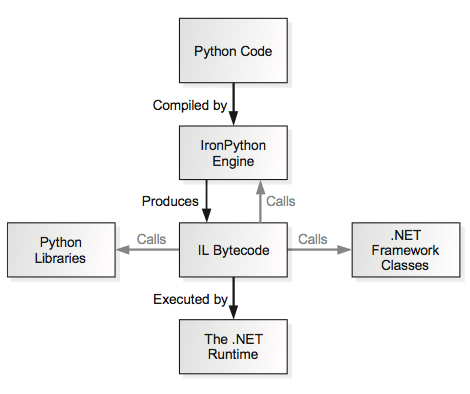
\includegraphics[scale=0.75]{IronPythonEngine}
\caption{How Python Code and Iron Python fit into .Net} \begin{center}
\citep{foord2009ironpython}
\end{center}
\label{Iron Python and .Net} 
\end{figure}
\end{center}

\subsection{Assemblies}
Assemblies are .NET libraries or executables. .NET consists of a great deal of these assemblies, in which the framework classes live, in the form of dlls. Because of the memory management and security features that .NET provides, code in .NET assemblies is called managed code. Assemblies contain code compiled from .NET languages into Intermediate Language (IL) bytecode. IL is run with the just-in-time (JIT) compiler for fast execution.

\section{Download and Install Iron Python}
There are different editors we can use to code Iron Python. In this course, we will be using: Python Tools for Visual Studio. To be able to run the code presented in this chapter, we need the following components:
\begin{itemize}
\item A Python interpreter such as CPython or IronPython [required]
\item Visual Studio 2010 or 2012 [required]
\item PTVS [required]
\item libraries/SDK’s/Distro’s [optional] 
\end{itemize}
To download and install Python Tools for Visual Studio, do the following:
\begin{enumerate}
\item Getting a Python interpreter:
For a minimal Python install, you can grab CPython or IronPython
However, we recommend installing one of the main Distros.
Whether installed before or after PTVS, PTVS will pick up your Python Interpreter location automatically.  You can further configure this from inside VS.
\item Getting Visual Studio: 
Note: PTVS does not install into VS Express Editions (Express editions aren't pluggable) - however PTVS + the Integrated Shell essentially gives you a "VS Python Express".
Your choices for Visual Studio are:
\begin{itemize}
\item Free: Get the VS 2010 Integrated Shell 
\item Free: Get the VS 2012 Isolated Shell + Integrated Shell 
\item Or the Full Visual Studio product
\begin{itemize}
\item Free: Get it through BizSpark (a program for startups)
\item Free: Get it through DreamSpark (for schools/students) 
\item Free: Get it through your school: You might already have a license for VS.
\end{itemize}
\end{itemize}
Note: If you have an older version of IronPython Tools or PTVS, please remove it first!
\end{enumerate}

\section{Iron Python for Python Programmers}
IronPython is a full implementation of Python. If you’ve already programmed with Python, there’s nothing to stop you from experimenting with IronPython immediately. The important question is, why would a Python programmer be interested in using IronPython? The answer is twofold: the platform and the platform. We know that, ini- tially, that might not make much sense, but bear with us. We’re referring first to the underlying platform that IronPython runs on—the CLR. Second, along with the run- time comes the whole .NET framework, a huge library of classes a bit like the Python standard library. The CLR is an interesting platform for several reasons. The CLR has had an enor- mous amount of work to make it fast and efficient. Multithreaded programs can take full advantage of multiple processors, something that CPython programs can’t do. Because of the close integration of Iron- Python with the CLR, extending IronPython through C\# code is significantly easier than extending CPython with C. There’s no C API to contend with; you can pass objects back and forth across the boundary without hassles and without reference counting16 to worry about. On top of all this, .NET has a concept called AppDomains. AppDomains allow you to run code with reduced privileges, such as preventing it from accessing the filesystem, a feature that has long been missing from CPython.

\begin{table}
\caption{Common .Net assemblies and namespaces}
\begin{tabular}{|p{4cm}|p{10cm}|}
\hline
System & Contains the base .NET types, exceptions, garbage collection classes, and much more.\\
\hline
System.Data & Classes for working with databases, both high and low level. \\
\hline
System.Drawing & Provides access to the GDI+ graphics system. \\
\hline
System.Management & Provides access to Windows management information and events (WMI), useful for system administration tasks. \\
\hline
System.Environment & Allows you to access and manipulate the current environment, like command-line arguments and environment variables. \\
\hline
System.Diagnostics & Tracing, debugging, event logging, and interacting with processes.\\
\hline
System.XML & For processing XML, including SOAP, XSL/T and more. \\
\hline
System.Web & The ASP.NET web development framework.\\
\hline
System.IO & Contains classes for working with paths, files, and directories. Includes classes to read and write to filesystems or data streams, synchronously or asynchronously. \\ \hline
Microsoft.Win32 & Classes that wrap Win32 common dialogs and components including the registry. \\ \hline
System.Threading System.Text & Classes needed for multithreaded application development. Classes for working with strings (such as StringBuilder) and the Encoding classes that can convert text to and from bytes.\\ \hline
System.Windows.Forms & Provides a rich user interface for applications. \\ \hline
System.Windows & The base namespace for WPF, the new GUI framework that’s part of .NET 3.0. \\ \hline
System.ServiceModel & Contains classes, enumerations, and interfaces to build Windows Communication Foundation (WCF) service and client applications. \\ \hline
\end{tabular}
\end{table}

\chapter{Binary Trees}
We have introduced and used several sequential structures throughout the text such as the array, Python list, linked list, stacks, and queues. These structures organize data in a linear fashion in which the data elements have a “before” and “after” relationship. They work well with many types of problems, but some problems require data to be organized in a nonlinear fashion. In this chapter, we explore the tree data structure, which can be used to arrange data in a hierarchical order. Trees can be used to solve many different problems, including those encountered in data mining, database systems, encryption, artificial intelligence, computer graphics, and operating systems.

\section{The Tree Structure}
A tree structure consists of nodes and edges that organize data in a hierarchical fashion. The relationships between data elements in a tree are similar to those of a family tree: “child,” “parent,” “ancestor,” etc. The data elements are stored in nodes and pairs of nodes are connected by edges. The edges represent the relationship between the nodes that are linked with arrows or directed edges to form a hierarchical structure resembling an upside-down tree complete with branches, leaves, and even a root.
Formally, we can define a tree as a set of nodes that either is empty or has a node called the root that is connected by edges to zero or more subtrees to form a hierarchical structure. Each subtree is itself by definition a tree.
A classic example of a tree structure is the representation of directories and subdirectories in a file system. The top tree in Figure 13.1 illustrates the hierar- chical nature of a student’s home directory in the UNIX file system. Trees can be used to represent structured data, which results in the subdivision of data into smaller and smaller parts. A simple example of this use is the division of a book into its various parts of chapters, sections, and subsections, as illustrated by the bottom tree in Figure 13.1. Trees are also used for making decisions. One that you are most likely familiar with is the phone, or menu, tree. When you call customer service for most businesses today, you are greeted with an automated menu that you have to traverse. The various menus are nodes in a tree and the menu options from which you can choose are branches to other nodes.

\chapter{Search Trees}

\part{ALGORITHMS: HOW COME?}
\chapter{Basic Sorting Algorithms}
\chapter{Basic Searching Algorithms}

\bibliographystyle{plain}
\bibliography{DSA}
\end{document}
